% This is the Reed College LaTeX thesis template. Most of the work
% for the document class was done by Sam Noble (SN), as well as this
% template. Later comments etc. by Ben Salzberg (BTS). Additional
% restructuring and APA support by Jess Youngberg (JY).
% Your comments and suggestions are more than welcome; please email
% them to cus@reed.edu
%
% See http://web.reed.edu/cis/help/latex.html for help. There are a
% great bunch of help pages there, with notes on
% getting started, bibtex, etc. Go there and read it if you're not
% already familiar with LaTeX.
%
% Any line that starts with a percent symbol is a comment.
% They won't show up in the document, and are useful for notes
% to yourself and explaining commands.
% Commenting also removes a line from the document;
% very handy for troubleshooting problems. -BTS

% As far as I know, this follows the requirements laid out in
% the 2002-2003 Senior Handbook. Ask a librarian to check the
% document before binding. -SN

%%
%% Preamble
%%
% \documentclass{<something>} must begin each LaTeX document
\documentclass[12pt,twoside]{reedthesis}
% Packages are extensions to the basic LaTeX functions. Whatever you
% want to typeset, there is probably a package out there for it.
% Chemistry (chemtex), screenplays, you name it.
% Check out CTAN to see: http://www.ctan.org/
%%
\usepackage{graphicx,latexsym}
\usepackage{amsmath}
\usepackage{amssymb,amsthm}
\usepackage{longtable,booktabs,setspace}
\usepackage{chemarr} %% Useful for one reaction arrow, useless if you're not a chem major
\usepackage[hyphens]{url}
% Added by CII
\usepackage{hyperref}
\usepackage{lmodern}
\usepackage{float}
\floatplacement{figure}{h}
% End of CII addition
\usepackage{rotating}

% Next line commented out by CII
%%% \usepackage{natbib}
% Comment out the natbib line above and uncomment the following two lines to use the new
% biblatex-chicago style, for Chicago A. Also make some changes at the end where the
% bibliography is included.
%\usepackage{biblatex-chicago}
%\bibliography{thesis}


% Added by CII (Thanks, Hadley!)
% Use ref for internal links
\renewcommand{\hyperref}[2][???]{\autoref{#1}}
\def\chapterautorefname{Chapter}
\def\sectionautorefname{Section}
\def\subsectionautorefname{Subsection}
% End of CII addition

% Added by CII
\usepackage{caption}
\captionsetup{width=5in}
% End of CII addition

% \usepackage{times} % other fonts are available like times, bookman, charter, palatino

% Syntax highlighting #22

% To pass between YAML and LaTeX the dollar signs are added by CII
\title{Proto-Solutrean lithic technology of Western Iberia: sites of Vale Boi and Lapa do Picareiro}
\author{Joana Belmiro}
% The month and year that you submit your FINAL draft TO THE LIBRARY (May or December)
\date{May 2020}
\division{Faculdade de Ciências Humanas e Sociais}
\advisor{João Cascalheira}
\institution{Universidade do Algarve}
\degree{Mestrado em Arqueologia}
%If you have two advisors for some reason, you can use the following
% Uncommented out by CII
% End of CII addition

%%% Remember to use the correct department!
\department{Arqueologia}
% if you're writing a thesis in an interdisciplinary major,
% uncomment the line below and change the text as appropriate.
% check the Senior Handbook if unsure.
%\thedivisionof{The Established Interdisciplinary Committee for}
% if you want the approval page to say "Approved for the Committee",
% uncomment the next line
%\approvedforthe{Committee}

% Added by CII
%%% Copied from knitr
%% maxwidth is the original width if it's less than linewidth
%% otherwise use linewidth (to make sure the graphics do not exceed the margin)
\makeatletter
\def\maxwidth{ %
  \ifdim\Gin@nat@width>\linewidth
    \linewidth
  \else
    \Gin@nat@width
  \fi
}
\makeatother

\renewcommand{\contentsname}{Table of Contents}
% End of CII addition

\setlength{\parskip}{0pt}

% Added by CII

\providecommand{\tightlist}{%
  \setlength{\itemsep}{0pt}\setlength{\parskip}{0pt}}

\Acknowledgements{

}

\Dedication{

}

\Preface{

}

\Abstract{
The present study aims to answer the question: what impact did the Heinrich 2 event have on the technological organization of human communities, at the onset of the last glacial maximum, in south western Iberia? The impact of this event on the Gravettian-Soluttrean transition has been previously suggested (Bradtmöller et al., 2012). However, the existing models do not consider the Proto-Solutrean technocomplex as an individual phase for this transition (Cascalheira and Bicho, 2013).

\par

To address this question, this study analysed the lithic assemblages from Vale Boi (south Portugal) and Lapa do Picareiro (central Portugal). We aimed to understand the technological patterns and raw material exploitation during the Proto-Solutrean, and test the existing models with assemblages from recently excavated sites, while expanding the geographic range.

The analysis followed a technologic and morphologic attribute approach. The retrieved data was then analysed through descriptive statistics in R environment.

Results show the existence of two occupations within the assemblages. The first, with high frequency of quartz use for bladelet production, seems to reflect a terminal gravettian horizon. The appearance of Vale Comprido technology and lower quartz frequencies in a second moment in Vale Boi, seem to represent a proto-solutrean occupation. The second horizon in Lapa do Picareiro, with the presence of technology similar to Vale Comprido but with low flattening ratios may be attributed to a Proto-Solutrean or an Early Solutrean occupation.

The Terminal Gravettian and Proto-Solutrean seem to be chronologically different phases, in concordance with the Three-Phase model for the Proto-Solutrean (Zilhão, 1997a). The similarities between Vale Boi and the Estremadura may be explained by the expansion of social networks (Cascalheira and Bicho, 2013). Associated with the dominance of different technological patterns and intensive use of quartz, we may understand these horizons as a moment of cultural reorganization, onset by environmental pressures.

~

\textbf{Keywords:} Upper Paleolithic; Attribute analysis; Raw material exploitation; Climatic changes.
}

\Resumo{
O objetivo desta tese é responder à seguinte pergunta: que impacto teve o evento climático Heinrich 2 (HE 2) na organização tecnológica das comunidades de caçadores-recolectores no início do último máximo glacial (LGM), no sudoeste peninsular?

\par

Esta questão está intimamente ligada ao entendimento de certos eventos climáticos abruptos, tais como os eventos de Heinrich ou os Estados Glaciares, com a substituição de culturas ao longo do Paleolítico Superior (Bradtmöller et al., 2012). Um destes momentos de substituição correlaciona a passagem do Gravetense para o Solutrense com o evento HE 2 e com o Estádio Glacial 3, possivelmente sobreposta pelo LGM. Neste paradigma, as mudanças climáticas desencadeiam mudanças sociais, através do colapso de tradições que depois são reorganizadas, de forma a corresponder às novas condições ambientais e paisagísticas. No entanto, nos modelos existentes, o Proto-Solutrense não surge como um tecnocomplexo individualizado, existindo assim uma lacuna no entendimento atual do processo de transição entre os dois horizontes culturais supramencionados (Cascalheira and Bicho, 2013).

O Proto-Solutrense, representado sobretudo na Estremadura Portuguesa, é entendido como um tecnocomplexo de transição, ocorrendo entre os 26 300 cal BP e 25 400 cal BP, e caracterizado por mudanças na tecnologia e preferência de matérias-primas, existindo dois modelos para a sua evolução: modelo em duas etapas e modelo em três etapas (Zilhão, 1997a).

O modelo em duas etapas considera a existência do Gravetense Final e Proto-Solutrense, caracterizado pelo uso intensivo de quartzo e estratégias de produção para obtenção de lamelas em núcleos carenados e obtenção de suportes convergentes para pontas de Vale Comprido, sendo no entanto, caracterizado por uma alta variabilidade interna. O modelo em três etapas consiste na evolução do Gravetense Final para uma etapa intermédia (no modelo das duas etapas considerada uma fácies funcional do Proto-Solutrense), caracterizada pelo uso intensivo do quartzo, estratégias de redução para obtenção de lamelas em núcleos carenados, seguida de uma fase proto-solutrense caracterizada pela diminuição do uso do quartzo e estratégias de redução para obtenção de suportes convergentes para pontas de Vale Comprido.

O conhecimento atual do Proto-Solutrense apresenta-se truncado, no entanto, pela antiguidade de algumas escavações e a sua restrição geográfica à Estremadura Portuguesa.

De forma a responder à questão supramencionada, assim como contribuir para o conhecimento do Proto-Solutrense no sudoeste Peninsular, foram analisados os conjuntos líticos de Vale Boi (sul de Portugal) e Lapa do Picareiro (Portugal central), ambos escavados nos últimos 20 anos com recurso a estações totais.

Esta análise teve a finalidade de entender os padrões tecnológicos e de exploração do território durante o Proto-Solutrense, através dos seguintes objetivos: 1) entender e explicar os padrões tecnológicos e de preferência de matérias-primas intra-sítio; 2) entender a existência de fases dentro das coleções estudadas; 3) testar os modelos de transição existentes para a Estremadura e entender possíveis variações geográficas.

A análise seguiu uma abordagem de atributos tecnológicos e morfológicos, com base em estudos aplicados para coleções do Paleolítico Superior, e seguindo os conceitos definidos na literatura especializada (\emph{e.g.} Tixier 1980; 1963; Andrefsky 1998; Inizan 1999). Esta foi seguida de uma fase de tratamento estatístico através de estatística descritiva efetuada em ambiente R. A escrita da tese foi também realizada em R, através do pacote Rmarkdown.

Os resultados permitiram individualizar duas fases dentro de ambos os contextos: uma fase inferior refletida na camada U e T inferior (Lapa do Picareiro) e camada 5 inferior (Vale Boi), atribuída ao Gravetense Terminal; fase superior, refletida nos níveis centrais da camada T (Lapa do Picareiro) e topo da camada 5 e 4E (Vale Boi), atribuída ao Proto-Solutrense. Estas mantêm padrões tecnológicos semelhantes: obtenção de produtos alongados e lascas através de núcleos simples ou prismáticos, com plataformas lisas e estratégias unidirecionais. Estas estratégias foram aplicadas de forma semelhante ao sílex e quartzo.

A fase gravetense terminal é caracterizada pelo uso extensivo de quartzo (\textasciitilde50\%), maioritariamente para a obtenção de lamelas. Apesar de em ambos os sítios não existir a presença de raspadeiras carenadas ou elementos carenados, típicos do Gravetense Terminal (Almeida, 2000), a presença de lamelas curvas intui para a utilização desta estratégia de redução.

A fase proto-solutrense é caracterizada pela diminuição do uso de quartzo (continuando, no entanto, com uma frequência de \textasciitilde30\%) e aparecimento de uma sequência de redução para obtenção de suportes de Vale Comprido. Estes suportes, depois transformados em pontas de Vale Comprido, são caracterizados por formas alongadas, convergentes e espessas, marcados por negativos dorsais unidirecionais e plataformas simples. Na Lapa do Picareiro, no entanto, em vez de suportes de Vale Comprido regista-se a presença de suportes com características semelhantes, mas com algumas diferenças, tais como índices de carenagem baixos, não tendo sido, portanto, considerados como Vale Comprido.

Estes padrões identificados em ambos os contextos dentro das coleções analisadas assemelham-se aos assinalados na Estremadura para ambas as fases (Zilhão, 1997a; Almeida, 2000).

A diferenciação entre estas fases é suportada também por dados cronológicos. A fase gravetense terminal parece ocorrer aos 27 mil anos cal BP na Lapa do Picareiro, e aos 26 mil anos cal BP em Vale Boi. A fase proto-solutrense ocorre aos 25 mil anos cal BP, podendo estender-se aos 24 mil anos cal BP no caso da Lapa do Picareiro.

Isto permite-nos sugerir que o modelo em três fases é aquele que melhor se adequa aos sítios estudados. A datação da ocupação mais recente da Lapa do Picareiro poderá, no entanto, representar uma fase de transição entre o Proto-Solutrense e o Solutrense Médio, uma fase ainda por identificar em Portugal (Zilhão, 1997a).

~

\textbf{Palavras-chave:} Paleolítico Superior; Análise de atributos; Exploração de matérias-primas; Alterações climáticas.
}

	\usepackage{caption}
\usepackage{flafter}
\captionsetup[figure]{font=footnotesize}
\captionsetup[table]{font=footnotesize}
\usepackage{indentfirst}
\setlength{\parindent}{20pt}
	\usepackage{booktabs}
\usepackage{longtable}
\usepackage{array}
\usepackage{multirow}
\usepackage{wrapfig}
\usepackage{float}
\usepackage{colortbl}
\usepackage{pdflscape}
\usepackage{tabu}
\usepackage{threeparttable}
\usepackage{threeparttablex}
\usepackage[normalem]{ulem}
\usepackage{makecell}
\usepackage{xcolor}
% End of CII addition
%%
%% End Preamble
%%
%
\begin{document}

% Everything below added by CII
  \maketitle

\frontmatter % this stuff will be roman-numbered
%\pagestyle{empty} % this removes page numbers from the frontmatter


  \begin{abstract}
    The present study aims to answer the question: what impact did the Heinrich 2 event have on the technological organization of human communities, at the onset of the last glacial maximum, in south western Iberia? The impact of this event on the Gravettian-Soluttrean transition has been previously suggested (Bradtmöller et al., 2012). However, the existing models do not consider the Proto-Solutrean technocomplex as an individual phase for this transition (Cascalheira and Bicho, 2013).
    
    \par
    
    To address this question, this study analysed the lithic assemblages from Vale Boi (south Portugal) and Lapa do Picareiro (central Portugal). We aimed to understand the technological patterns and raw material exploitation during the Proto-Solutrean, and test the existing models with assemblages from recently excavated sites, while expanding the geographic range.
    
    The analysis followed a technologic and morphologic attribute approach. The retrieved data was then analysed through descriptive statistics in R environment.
    
    Results show the existence of two occupations within the assemblages. The first, with high frequency of quartz use for bladelet production, seems to reflect a terminal gravettian horizon. The appearance of Vale Comprido technology and lower quartz frequencies in a second moment in Vale Boi, seem to represent a proto-solutrean occupation. The second horizon in Lapa do Picareiro, with the presence of technology similar to Vale Comprido but with low flattening ratios may be attributed to a Proto-Solutrean or an Early Solutrean occupation.
    
    The Terminal Gravettian and Proto-Solutrean seem to be chronologically different phases, in concordance with the Three-Phase model for the Proto-Solutrean (Zilhão, 1997a). The similarities between Vale Boi and the Estremadura may be explained by the expansion of social networks (Cascalheira and Bicho, 2013). Associated with the dominance of different technological patterns and intensive use of quartz, we may understand these horizons as a moment of cultural reorganization, onset by environmental pressures.
    
    ~
    
    \textbf{Keywords:} Upper Paleolithic; Attribute analysis; Raw material exploitation; Climatic changes.
  \end{abstract}
  \begin{resumo}
    O objetivo desta tese é responder à seguinte pergunta: que impacto teve o evento climático Heinrich 2 (HE 2) na organização tecnológica das comunidades de caçadores-recolectores no início do último máximo glacial (LGM), no sudoeste peninsular?
    
    \par
    
    Esta questão está intimamente ligada ao entendimento de certos eventos climáticos abruptos, tais como os eventos de Heinrich ou os Estados Glaciares, com a substituição de culturas ao longo do Paleolítico Superior (Bradtmöller et al., 2012). Um destes momentos de substituição correlaciona a passagem do Gravetense para o Solutrense com o evento HE 2 e com o Estádio Glacial 3, possivelmente sobreposta pelo LGM. Neste paradigma, as mudanças climáticas desencadeiam mudanças sociais, através do colapso de tradições que depois são reorganizadas, de forma a corresponder às novas condições ambientais e paisagísticas. No entanto, nos modelos existentes, o Proto-Solutrense não surge como um tecnocomplexo individualizado, existindo assim uma lacuna no entendimento atual do processo de transição entre os dois horizontes culturais supramencionados (Cascalheira and Bicho, 2013).
    
    O Proto-Solutrense, representado sobretudo na Estremadura Portuguesa, é entendido como um tecnocomplexo de transição, ocorrendo entre os 26 300 cal BP e 25 400 cal BP, e caracterizado por mudanças na tecnologia e preferência de matérias-primas, existindo dois modelos para a sua evolução: modelo em duas etapas e modelo em três etapas (Zilhão, 1997a).
    
    O modelo em duas etapas considera a existência do Gravetense Final e Proto-Solutrense, caracterizado pelo uso intensivo de quartzo e estratégias de produção para obtenção de lamelas em núcleos carenados e obtenção de suportes convergentes para pontas de Vale Comprido, sendo no entanto, caracterizado por uma alta variabilidade interna. O modelo em três etapas consiste na evolução do Gravetense Final para uma etapa intermédia (no modelo das duas etapas considerada uma fácies funcional do Proto-Solutrense), caracterizada pelo uso intensivo do quartzo, estratégias de redução para obtenção de lamelas em núcleos carenados, seguida de uma fase proto-solutrense caracterizada pela diminuição do uso do quartzo e estratégias de redução para obtenção de suportes convergentes para pontas de Vale Comprido.
    
    O conhecimento atual do Proto-Solutrense apresenta-se truncado, no entanto, pela antiguidade de algumas escavações e a sua restrição geográfica à Estremadura Portuguesa.
    
    De forma a responder à questão supramencionada, assim como contribuir para o conhecimento do Proto-Solutrense no sudoeste Peninsular, foram analisados os conjuntos líticos de Vale Boi (sul de Portugal) e Lapa do Picareiro (Portugal central), ambos escavados nos últimos 20 anos com recurso a estações totais.
    
    Esta análise teve a finalidade de entender os padrões tecnológicos e de exploração do território durante o Proto-Solutrense, através dos seguintes objetivos: 1) entender e explicar os padrões tecnológicos e de preferência de matérias-primas intra-sítio; 2) entender a existência de fases dentro das coleções estudadas; 3) testar os modelos de transição existentes para a Estremadura e entender possíveis variações geográficas.
    
    A análise seguiu uma abordagem de atributos tecnológicos e morfológicos, com base em estudos aplicados para coleções do Paleolítico Superior, e seguindo os conceitos definidos na literatura especializada (\emph{e.g.} Tixier 1980; 1963; Andrefsky 1998; Inizan 1999). Esta foi seguida de uma fase de tratamento estatístico através de estatística descritiva efetuada em ambiente R. A escrita da tese foi também realizada em R, através do pacote Rmarkdown.
    
    Os resultados permitiram individualizar duas fases dentro de ambos os contextos: uma fase inferior refletida na camada U e T inferior (Lapa do Picareiro) e camada 5 inferior (Vale Boi), atribuída ao Gravetense Terminal; fase superior, refletida nos níveis centrais da camada T (Lapa do Picareiro) e topo da camada 5 e 4E (Vale Boi), atribuída ao Proto-Solutrense. Estas mantêm padrões tecnológicos semelhantes: obtenção de produtos alongados e lascas através de núcleos simples ou prismáticos, com plataformas lisas e estratégias unidirecionais. Estas estratégias foram aplicadas de forma semelhante ao sílex e quartzo.
    
    A fase gravetense terminal é caracterizada pelo uso extensivo de quartzo (\textasciitilde50\%), maioritariamente para a obtenção de lamelas. Apesar de em ambos os sítios não existir a presença de raspadeiras carenadas ou elementos carenados, típicos do Gravetense Terminal (Almeida, 2000), a presença de lamelas curvas intui para a utilização desta estratégia de redução.
    
    A fase proto-solutrense é caracterizada pela diminuição do uso de quartzo (continuando, no entanto, com uma frequência de \textasciitilde30\%) e aparecimento de uma sequência de redução para obtenção de suportes de Vale Comprido. Estes suportes, depois transformados em pontas de Vale Comprido, são caracterizados por formas alongadas, convergentes e espessas, marcados por negativos dorsais unidirecionais e plataformas simples. Na Lapa do Picareiro, no entanto, em vez de suportes de Vale Comprido regista-se a presença de suportes com características semelhantes, mas com algumas diferenças, tais como índices de carenagem baixos, não tendo sido, portanto, considerados como Vale Comprido.
    
    Estes padrões identificados em ambos os contextos dentro das coleções analisadas assemelham-se aos assinalados na Estremadura para ambas as fases (Zilhão, 1997a; Almeida, 2000).
    
    A diferenciação entre estas fases é suportada também por dados cronológicos. A fase gravetense terminal parece ocorrer aos 27 mil anos cal BP na Lapa do Picareiro, e aos 26 mil anos cal BP em Vale Boi. A fase proto-solutrense ocorre aos 25 mil anos cal BP, podendo estender-se aos 24 mil anos cal BP no caso da Lapa do Picareiro.
    
    Isto permite-nos sugerir que o modelo em três fases é aquele que melhor se adequa aos sítios estudados. A datação da ocupação mais recente da Lapa do Picareiro poderá, no entanto, representar uma fase de transição entre o Proto-Solutrense e o Solutrense Médio, uma fase ainda por identificar em Portugal (Zilhão, 1997a).
    
    ~
    
    \textbf{Palavras-chave:} Paleolítico Superior; Análise de atributos; Exploração de matérias-primas; Alterações climáticas.
  \end{resumo}
  \hypersetup{linkcolor=black}
  \setcounter{tocdepth}{2}
  \tableofcontents

  \listoftables

  \listoffigures


\mainmatter % here the regular arabic numbering starts
\pagestyle{fancyplain} % turns page numbering back on

\hypertarget{introduction}{%
\chapter{Introduction}\label{introduction}}

The replacement of the gravettian technocomplex by the Solutrean, impacted by adverse climatic conditions during the Heinrich Event 2 (HE2), continues to be an essential topic to understand the Upper Paleolithic and Human adaptations to climatic changes. The Proto-Solutrean is, in this topic, an essential piece to understand how hunter-gatherer communities adapted, reinvented and destroyed their social and technologic organization which eventually allowed the development of the Solutrean. However, most of what is known for this technocomplex is still geographically constricted and lacking good chronological markers (Cascalheira and Bicho, 2013), which hampers the understanding of the Proto-Solutrean itself and its role in the Gravettian-Solutrean transition.

By understanding the need to better comprehend the Proto-Solutrean and how adverse climate impacted these communities, this study aims to answer the following question: what impact did the HE 2 have on the technological organization of human communities, at the onset of the Last Glacial Maximum (LGM), in south western Iberia? To do so, this study will analyse the lithic terminal gravettian/proto-solutrean assemblages of two recently excavated sites, with resource to total stations, Vale Boi (south of Portugal) and Lapa do Picareiro (central Portugal).

To answer this question, we aim to accomplish the following goals:
\begin{itemize}
\item
  Understand the technological organization of layers 5/4E of Vale Boi and U to Middle T from Lapa do Picareiro, by characterizing their technological patterns, reduction sequences and raw material use/preference patterns. The results will then be compared with the existing data from other proto-solutrean assemblages, mostly from the Portuguese Estremadura.
\item
  Identify possible terminal gravettian horizons or facies within the proto-solutrean occupations in Vale Boi and Lapa do Picareiro and their chronologies.
\item
  Test the proto-solutrean transition models (Two-phase and Three-phase) developed through results from the Estremadura to understand which model best explains the transition between the Final Gravettian to the Proto-Solutrean, and whether the model may be applied to other geographic areas outside of the Estremadura.
\end{itemize}
By accomplishing these goals, through the use of new data resulting from recent excavations, with good chronological markers and a wider geographic range (south of Portugal), we hope to contribute to the understanding of the Proto-Solutrean and the Gravettian-Solutrean transition in western Iberia.

The present thesis is organized in 7 chapters:
\begin{itemize}
\item
  Chapter 2, where we will discuss the impact of climatic changes on culture replacement, especially during the HE 2, describe the paleoclimate during this event and finally describe the Proto-Solutrean and its technological characteristics.
\item
  Chapter 3 which will introduce the archaeological sites used in the study with a brief description of their location and geological context, followed by an overview of excavation works, excavation methodology, human occupation through the several areas and layers, then focusing on the layers associated with terminal gravettian/proto-solutrean horizons.
\item
  Chapter 4, where we will overview the methodology employed in both the lithic and data analysis.
\item
  Chapter 5 which will consist on the description of the results obtained through the analysis of the assemblages from Vale Boi and Lapa do Picareiro, respectively. This will be organized by assemblage description, raw materials and technology.
\item
  Chapter 6 will focus on the discussion of the results presented in the previous chapter, comparing them to other results from proto-solutrean assemblages, mostly from the Portuguese Estremadura. In this chapter we will also discuss problematics which relate to the goals aforementioned.
\item
  Chapter 9 will consist of this study's conclusions, systematizing the analysis interpretations and discussion.
\end{itemize}
\hypertarget{human-adaptations-at-the-start-of-the-last-glacial-maximum}{%
\chapter{Human adaptations at the start of the last glacial maximum}\label{human-adaptations-at-the-start-of-the-last-glacial-maximum}}

\hypertarget{paleoclimate-paleoenvironment-and-human-adaptation-models}{%
\section{Paleoclimate, paleoenvironment and human adaptation models}\label{paleoclimate-paleoenvironment-and-human-adaptation-models}}

The integration of paleoclimatic and paleoenvironmental data on archaeological studies can be traced to the last quarter of the twentieth century, especially in Portugal, which was also a result of the embryonic stage of research and methodologies developed until that moment (Cascalheira, 2010). Nowadays, the ecological context and external pressures are seen as essential in order to understand human behavior and changes in the material culture, which is inevitably what is left behind (Thacker, 1996; Holst, 2017), especially when dealing with technocomplexes which are recognized as transitional climate-wise, such as the Proto-Solutrean (Almeida, 2000).

Some of the first attempts at reconstructing the paleoclimate in Portugal during the glacial era in the Upper Paleolithic were made by Roche (1971, 1977), through the results obtained by the analysis of fauna in the Portuguese Estremadura. In this model, the Iberian Peninsula did not go through dramatic climatic changes, unlike other areas in Europe, presenting instead milder conditions. This model has since been subject to many critics (Zilhão, 1997a; Almeida, 2000), through the postulation of harsher climatic conditions for the Iberian Peninsula during the Late Glacial.

Advances in paleoclimatic reconstruction, mainly from Greenland ice cores and deep-sea ice cores, have allowed the recognition of millennial-scale oscillations within Marine Isotopic Stages (MIS) 4, 3 and 2 in better detail. This permited obtaining a robust chronology and understanding of the climatic conditions that characterized the Late Pleistocene (Cascalheira and Bicho, 2013).

The Pleistocene was marked by a series of climatic events, with significant impact on western Europe, influencing most ecological aspects, from the environment and animal distribution: the Dansgaard-Oeschger stadials (D-O stadials), sometimes associated with the formation of ice-rafted debris (IRD) layers in the ocean, named Heinrich events (HEs) (Heinrich, 1988; Cascalheira and Bicho, 2013).

These abrupt climate changes also impacted the communities of hunter-gatherers, something visible in the archaeological record through the intensification and diversification in the technology and economy of lithic assemblages (Cascalheira and Bicho, 2013). In fact, there has been a significant amount of proposals suggesting a full synchronism between the onset of each Upper Paleolithic technocomplex and the occurrence of the most severe climate events (Cascalheira and Bicho, 2013). Bradtmöller \emph{et al.} (2012) suggest a direct relationship between three of the HEs (4, 3 and 2) and the substitution of Neanderthal populations with the emergence of the Aurignacian, the appearance of the Gravettian and the development of the Solutrean, respectively (Table \ref{tab:climatetable}). Based on the theoretical framework of Panarchy (Holling and Gunderson, 2002), the authors propose the Repeated Replacement Model (RRM), where the HEs are understood as the primary climatic triggers for population turnover, through the breakdown of communication networks and cultural traditions, which were subsequently reorganized under different socio-cultural conditions (Bradtmöller et al., 2012).

In this framework, the rapid climatic changes brought by the HE 2 were the trigger for the reorganization of human groups after the Gravettian. This led to the development of the Solutrean, marked by harsh conditions onset by the LGM. A technological continuum with clear succession between the two technocomplexes is seen, at least in Iberia (Bradtmöller et al., 2012), making the comprehension of these rapid climatic events of extreme importance for the understanding of human cultural change, specifically for the Proto-Solutrean and Solutrean.

~
\begin{table}[!h]

\caption{\label{tab:climatetable}Correspondence between Upper Paleolithic cultural phases (Aurignacian, Gravettian and Solutrean), Heinrich Events and D-O cycles, with respective chronology. Following dates and chronologies from Bradtmöller et al. (2012), Cascalheira and Bicho (2013), Sanchéz-Goñi and Harrison (2010).}
\centering
\fontsize{9}{11}\selectfont
\begin{tabular}[t]{ll>{\raggedright\arraybackslash}p{4cm}>{\raggedright\arraybackslash}p{4cm}}
\toprule
\textbf{Cultural Phase} & \textbf{Heinrich event} & \textbf{Chronology ka cal BP (Sanchéz-Goñi and Harrison 2010)} & \textbf{D-O cycle correspondence}\\
\midrule
Aurignacian & H4 & 40.2-38.3 & GS 8/9\\
Gravettian & H3 & 32.7-31.3 & GS 4/5\\
Solutrean & H2 & 26.5-24.3 & GS 2/3\\
\bottomrule
\end{tabular}
\end{table}
~

As such, D-O stadials are described as rapid cyclical climatic changes, characterized in Greenland by an oscillation between warmer and cooler moments. Within the D-O stadials, the term stadial is used to refer to the cold intervals, while the term interstadial is used to describe warmer periods (Sanchez Goñi and Harrison, 2010).

The HEs represent the expansion of polar water from the icebergs that broke off from the Laurentide Fenno-Scandinavian ice sheet and melted into the North Atlantic (Elliot et al., 2001). These events have been detected in deep-sea cores by the presence of IRD, high percentages of polar water foraminifer (\emph{N. pachyderma}), increase in magnetic susceptibility and decreases in sea surface temperatures ({\textbf{???}}; Goñi et al., 2000; Naughton et al., 2007; Fletcher, 2008; Sanchez Goñi and Harrison, 2010). Similar to the D-O stadials, HE events are also periodical, with 6 identified HE events, occurring every 10-6 k years, since 63.2 ka, following the GICC05 chronology as applied by Sanchez-Goñi and Harrison (2010), with durations as long as 3 k years and as short as 1.5 k.

These rapid climate changes, both D-O stadials and HEs are, as mentioned above, superimposed by longer-term climate patterns - the MIS - which correspond to intervals of more (MIS 4 and 2) or less (MIS 3) permanent ice cover in the polar ice caps. Conventionally, MIS 4 is correlated with D-O 19, MIS 3 with D-O 17, while MIS 2 shows variable correlations, depending on the author, although the present study is adopting the consensus view that it corresponds to the boundary between D-O 4 and D-O 3 (Sanchez Goñi and Harrison, 2010).

The correlation of HE 2 with the LGM is problematic due to the wide variety of dates available for this latter event, with its onset sometimes superimposed by the start of HE 2, and others pushed to much later, starting at the middle of HE 2 (Sanchez-Goñi and Harrison 2010). Even so, there seems to be an apparent correlation between the HE 2 and the LGM, the latter having a wider temporal extension ({\textbf{???}}; Mix et al., 2001; Clark et al., 2009; Bradtmöller et al., 2012).

HE's also seem to have some internal variability, which complexifies our understanding of it, as is the case with HE 2 on the western Iberian coast, with two identified phases: a first phase with increase in \emph{N. pachyderma} percentages and presence of IRD, which suggest a decrease of sea surface temperatures, followed by a phase where polar foraminifera percentages decrease, suggesting a more extensive seasonal variability in sea surface conditions (Turon et al., 2003; Naughton et al., 2007).

This climatic variability is felt not only at a chronological level but also at a geographic level. Land conditions (achieved by the analysis of pollen samples within the cores) seem to have been different in northern Iberia and southwestern Iberia as shown through the recovered cores in the southwestern area off Portugal: SU81-18 (Turon et al., 2003); and to the northwestern Iberia, off Galicia: MD99-2331 and MD03-2697 (Naughton et al., 2007, 2016). In conjunction with other climate-proxy data, such as the Greenland ice cores, palynological studies, charcoal studies and faunal analysis, these records have allowed for the characterization of the paleo-climatic conditions of western and southern Iberia during the Pleistocene (Sanchez Goñi and Harrison, 2010; Cascalheira and Bicho, 2013).

Records indicate that during HEs, and with particular severity in the HE 2, western and southern Iberia must have experienced abrupt environmental changes, which altered the location, abundance and availability of resources for the communities of hunter-gatherers (Cascalheira and Bicho, 2013).

Regarding vegetation, the data from sites with archaeological layers dated to the HE 2 time-span (e.g.~Lapa do Anecrial) show that steppe landscapes and open pine woodlands prevailed. Meanwhile, a diversity of species was maintained by the existence of refuge zones, as warm-adapted vegetation became constrained in those areas, possibly located near the coast or in sunlit slopes of protected areas (González-Sampériz et al., 2010).

Pollen analyses from deep-sea cores show, for northwestern Iberia (cores MD99-2331 and MD03-2697), the existence of two periods, marked by the dominance of herbaceous communities (shrubs and grasses), along with a \emph{Pinus} forest reduction, which indicates a cold and humid continental climate. The second part of HE 2 however, is characterized by \emph{Pinus} forest expansion, hinting for less cold conditions (Naughton et al., 2007). For southwestern territory (Figure \ref{fig:su8118}), pollen analyses show the expansion of semi-desert shrubberies, which suggest increased dry conditions during the full extension of the HE 2, although, unlike results for northern Iberia, \emph{Pinus} forests do not seem to have decreased (Turon et al., 2003). Alike the data obtained from archaeological sites, pollen analyses from cores show the presence of a variety of deciduous trees and shrubs (\emph{Quercus}, \emph{Corylus} and \emph{Alnus}), corroborating the idea of north and southern Iberia as refugium zones for temperate-climate species (Turon et al., 2003).
\begin{figure}[H]

{\centering \includegraphics[width=0.8\linewidth]{figure/Turon2003_SU81-18} 

}

\caption{Diagram showing the main pollen and spore taxa and dinoflagellate cyst specimens per depth (Turon et al. 2003).}\label{fig:su8118}
\end{figure}
Faunal analyses, specifically micro-fauna, show that these changes in habitats were followed by a change in animal incidence, with the increase of steppe adapted species, although warmer-adapted ones continued to appear in the archaeological record (Almeida, 2000). The results for mammalian fauna analyses show a dominant pattern for pronounced resilience of most animal species in the archaeological record, with a few fluctuations in the presence of wild boar, which may represent environmental responses to the rapid climate changes (Haws, 2012). Brugal and Valente (2007) also report mammalian fauna differences within the HE 2, with a broader extinction of local carnivores, while herbivore frequency remains mostly the same, with significant shifts in their spatial distribution.

Thus, despite results clearly showing that the HE 2 caused abrupt modifications in the landscape and climate of western and southern Iberia (Cascalheira and Bicho, 2013), this territory still functioned as a refuge even during the colder periods (Gómez and Lunt, 2007; Carrión et al., 2010), in sheltered areas scattered throughout the landscape (Schmidt et al., 2012).

Although there are several paleoclimate sources which have allowed the reconstruction of the climate during the HE 2, this data cannot be fully integrated in the RRM model, to explain the emergence of the Solutrean by substitution of the Gravettian. The RRM model does not account for the Proto-Solutrean, possibly identifying it as either part of the Gravettian or Solutrean. In a way this reflects the current understanding of the Proto-Solutrean as a transitional stage between the other two technocomplexes, failing to recognize it as an independent unit.

However, in order to fully understand the impact of the HE 2 and the environmental changes on the replacement of the gravettian technocomplex by the Solutrean as mentioned above, the Proto-Solutrean needs to be understood and regarded as an independent unit, as a means to understand its role in the RRM. This issue has been addressed by Cascalheira and Bicho (2013), where within the RRM, the authors suggest the Proto-Solutrean as a moment of creative destruction (Holling, 2001), which allowed the separation from the Gravettian cultural system to the development of a new structure, the Solutrean. There is, however, the need for more technological and chronological data in order to understand how the many different pieces fit together in this framework.

As such, the Proto-Solutrean stands as an essential technocomplex to understand human adaptations to climatic and environmental changes within the Upper Paleolithic.

\hypertarget{proto-solutrean-origins-and-the-portuguese-model}{%
\section{Proto-Solutrean: origins and the Portuguese model}\label{proto-solutrean-origins-and-the-portuguese-model}}

Cultural horizons within the archaeological record have been traditionally defined through the characteristics and typologies of lithic materials. The same is true for the Upper Paleolithic sequence, which in Europe was the result of several archaeological campaigns in southwestern France. The stratigraphic organization and sequence of the latter became the reference model across the continent (Zilhão, 1997a).

Following this paradigm, the transition between the Gravettian and Solutrean was, for most of the second half of the twentieth century, based on the stratigraphy of Laugerie-Haute, in France, and thus defined in a four-stage process: Perigordian VII, Aurignacian V, Proto-Solutrean, Lower Solutrean. This succession of stages was understood as the substitution of human people and culture through processes of diffusion and migration, a paradigm present in the archaeological thought before the 1960s, and which changed drastically with the development of the New Archaeology ({\textbf{???}}) with new ways of seeing the past and archaeology ({\textbf{???}}). This new theoretical framework allowed the traditional cultural horizon sequences to be understood as the result of technological development, which did not necessarily imply the substitution of people (Zilhão et al., 1999). The impact of these new frameworks can be seen, for example, in the interpretation of the Perigordian VII, the first stage in the Gravettian-Solutrean transitional process. Nowadays, it is known that the Perigordian VII is, in fact, the final stage of the Gravettian (Zilhão, 1997a).

The Aurignacian V, meanwhile, has been a slightly more complicated subject. Its identification was based on the presence of thick-nosed endscrapers, a technological characteristic that represented the presence of Aurignacian communities, and thus, moments of population substitution and migration in the site (Zilhão, 1997a; Almeida, 2000). Part of the problem was also that this level was only known in one site in France.

The study of materials from old excavations by Manuel Heleno in Rio Maior (Portuguese Estremadura), and new archaeological works in the same region, in the 1980s, revealed assemblages from the Upper Paleolithic, some with levels of typological characteristics which paralleled those of Laugerie Haute. These projects allowed one of the most comprehensive descriptions of the Upper Paleolithic occupations in Portugal, and the understanding of the Gravettian-Solutrean transition in more detail, including the problematic Aurignacian V (Zilhão, 1994; Almeida, 2000).

The Proto-Solutrean has thus been described as a transitional technocomplex from Gravettian to Solutrean technologies, through a process of local development, and synchronous to all of the Southwestern Europe (Aquitaine, Pyrenees, Languedoc and the Iberian Peninsula) (Zilhão et al., 1999).

In total, 10 sites with either Proto-Solutrean assemblages or transitional characteristics were identified in the Portuguese Estremadura area (although not all have been dated; Figure \ref{fig:protomap}). Table \ref{tab:protodates} shows the dates for proto-solutrean occupations in Portugal, including the sites analyzed in this study.

This set of dates from sites such as Anecrial, Terra do Manuel (layer 2s), Alecrim, Buraca Escura (layer 2e) and Lagar Velho (since other dates show either values which look like outliers or have extremely high standard deviations) place the transition as happening between 26.2 ka cal BP and 25.4 ka cal BP (calibrated dates from Zilhão 1997, using IntCal 13 through Oxcal online), where the lowest boundary represents the beginning of the Final Gravettian and the highest the ending of the Proto-Solutrean (Zilhão, 1997a, 2000; Zilhão et al., 1999).

The understanding of the Gravettian-Solutrean transition through several phases, each with its technological characteristics and patterns, through the techno-typological characteristics of assemblages from key sites, have allowed for the creation of two models: the Two-stage model and Three-stage model (Zilhão, 1994, 1997a; Zilhão et al., 1999).
\begin{figure}[H]

{\centering \includegraphics[width=0.8\linewidth]{figure/map_proto_solutrean} 

}

\caption{Location of Proto-Solutrean sites in Portugal, including the two sites analysed in this study.}\label{fig:protomap}
\end{figure}
The Two-stage model (Figure \ref{fig:twophase}) starts with a final gravettian stage, characterized by a moderate use of quartz (\textasciitilde15\%), production of truncated backed bladelets and proto-magdalenian retouch blades, where we find Terra do Manuel (old excavations and layer 2s), Cabeço de Porto Marinho III (CPM III), Cabeço de Porto Marinho II (CPM II) and Buraca Escura (layer 2e) (Zilhão, 1997a). The second stage is the Proto-Solutrean, frequently characterized by a high percentage of quartz use (\textasciitilde30\%), rare presence of backed bladelets or, when retouch is present, being marginal, and the production of Vale Comprido points, the technocomplex's index fossil (Zilhão and Aubry, 1995; Zilhão, 1997a; Almeida, 2000). For the production of these tools, the Proto-Solutrean shows three different operative sequences: one for the production of Vale Comprido points, through the removal of elongated blanks with convergent profiles and thick platforms; another for the production of blades, of gravettian tradition; and another for the production of bladelets, probably obtained through the exploitation of thick endscapers or carinated elements. Proto-solutrean phase assemblages were identified in Vale Comprido -- Encosta, Terra do José Pereira, Vales da Senhora da Luz (although Vale Comprido points are absent from the assemblage), Terra do Manuel (layer 2), Buraca Escura (layer 2b), Anecrial (layer 2) and Gato Preto (group C) (Zilhão, 1997a).

Vale Comprido points are described as robust pieces, with a thickness ranging the 4-8 mm, width around 20 mm and length of about 50 mm, though in some cases it may reach 80 mm, and platform thickness of 5-20 mm. They are often characterised by convergent shapes, triangular cross- sections and plain platforms, often having a high elongation ratio, although not necessarily falling into the blade category (see Chapter 4). They can also be categorized regarding retouch, with the identification of 3 groups: 1) thinning of the platform; 2) extensive retouch across the edges, including the tip; 3) an intermediate type with only partial retouch on the edges along the platform or at the tip (Zilhão and Aubry, 1995; Zilhão, 1997a). The Vale Comprido points have been used to describe the technological transition between the Proto-Solutrean and the Solutrean. In this case, these points are seen as an element of discontinuity with the previous technocomplex, where the organic points armed with microliths from the Gravettian are replaced by lithic points, with enough similarities to the \emph{pointes à face plane} of the Middle Solutrean to be understood as a technological development (Zilhão, 2013).

The Three-stage model (Figure \ref{fig:threephase}) maintains the first final gravettian stage and its defining characteristics but subdivides the following proto-solutrean stage in two. As such, there is an intermediate stage characterized by the intensive use of quartz (\textasciitilde30\%), which corresponds to Laugerie Haute's Aurignatian V, migrating the assemblages from Terra do Manuel (layer 2s), CPM III, CPM II and Buraca Escura (layer 2b) to this phase. The third stage is the Proto-Solutrean, where quartz use diminishes. In this model, the Vale Comprido points and associated reduction sequence may appear in either of the last two stages (Zilhão, 1997a). However, Almeida (2000) has noted that the aurignacian V/terminal gravettian assemblages from the Estremadura seem to lack Vale Comprido technology (Almeida, 2000). It may seem, thus, that this type of technology is a proto-solutrean innovation.
\begin{figure}[H]

{\centering \includegraphics[width=0.7\linewidth]{figure/Two-phasemodel} 

}

\caption{Two-phase model for Gravettian to Proto-Solutrean transition, with site and archaeological level correlated with each phase. Adapted from Zilhão (1997). Model dates calibrated with curve IntCal13, using OxCal 4.1.7 (online).}\label{fig:twophase}
\end{figure}
\begin{figure}[H]

{\centering \includegraphics[width=0.7\linewidth]{figure/Three-phasemodel} 

}

\caption{Three-phase model for Gravettian to Proto-Solutrean transition, with site and archaeological level correlated with each phase. Adapted from Zilhão (1997). Model dates calibrated with curve IntCal13, using OxCal 4.1.7 (online).}\label{fig:threephase}
\end{figure}
~

Alternatively, in the Two-phase model, the Aurignacian V, is understood as a functional facies, related to specialized occupations and production activities within the technocomplex, through the observation of the coexistence of prismatic core exploitation and carinated core exploitation. The fact that both showed extraction of blades and bladelets, the latter exploitation was interpreted not an independent system as thought at Laugerie Haute (Zilhão, 1997a; Zilhão et al., 1999). In fact, Zilhão (1994, 1997a) has questioned the stratigraphic reality of the Aurignacian V from Laugerie-Haute, interpreting it only as a typology separation due to poor stratigraphic integrity.

Almeida (2000) interprets the diagnostic aurignacian thick-nosed endscrapers as carinated cores, with no correlation to the aurignacian technocomplex, suggesting instead the substitution of the term Aurignacian V for Terminal Gravettian. Following previous works (Almeida, 2000; Cascalheira and Bicho, 2013; Benedetti et al., 2019), when referring to the Aurignacian V, whether as a functional facies (Two-stage model) or as an intermediate stage (Three-stage model), the present study will apply the term Terminal Gravettian instead.

One of the main differences between the models aforementioned is connected to the lithic assemblage's internal variability. In this case, the Three-stage model diminishes this internal variability by attributing chronological significance to the Terminal Gravettian (Almeida, 2000). The Three-Phase model causes some sites to float between the Terminal Gravettian and Proto-Solutrean without an exact phase attribution (such as Terra do José Pereira, Vales da Senhora da Luz, Anecrial and Gato Preto), due to lack of necessary information or specialized character of their occupations (Zilhão, 1997a).The Two-phase, because it accepts higher internal variability but also limits the number of options, guarantees that a specific phase can be attributed to all sites.

However, in the last decades, the Three-Phase model has been the most accepted, and the Terminal Gravettian phase is nowadays well-characterized technologically in Estremadura as a moment of chronological significance (Almeida, 2000), even if from a chronographic perspective, it lacks irrefutable evidence as shown by Cascalheira and Bicho (2013), for which the authors present two causes: most available radiocarbon dates, spreading through the entire HE 2 and covering the proto-solutrean's time-span come from sites with assemblages which are attributed to the Terminal Gravettian (with the exception of Vale Boi and possibly Lapa do Picareiro); absolute ages of sites with a strong Vale Comprido component remain unknown.

Although this has been explained by some authors, for example Aubry et al. (2011) and ({\textbf{???}}), as the result of strong erosive processes affecting the archaeological sites during the HE 2, other authors (Haws, 2012) fail to recognize such an extensive erosion.

Regardless of what model is accepted, the Proto-Solutrean, from the beginning of its transitional stage, stands as a technocomplex with technological innovations. These are reflected in the manufacture of Vale Comprido points and a complete operative sequence for their production, but marked by a high degree of technological variability in their lithic assemblages (Zilhão, 1997a; Zilhão et al., 1999; Almeida, 2000).

This variability has been interpreted as a technological race in response to the environmental modifications taking course during the HE 2 (Cascalheira and Bicho, 2013). The authors suggest that, in order to correspond to the external pressures, there may have been the need to diversify the economic strategies in use until that moment. The high exploitation of quartz, for example, formerly a secondary raw material, and the use of similar reduction strategies between quartz and chert, might represent one such economic response. The same possibly applies to the use of unprecedented raw materials, as is the case of the proto-solutrean levels in Vale Boi, where there is the presence of previously unknown raw materials, used mainly in the manufacture of Vale Comprido points (Marreiros, 2009; Belmiro et al., n.d.). Likewise, alterations recorded in territoriality patterns for the Proto-Solutrean can be interpreted has extensive regional networks and may be related to modifications in the landscape that occurred during the HE 2 (Cascalheira and Bicho, 2013; Cascalheira, 2019).

These technological and behavioral changes, when understood under the light of the Repeated Replacement Model previously discussed (Bradtmöller et al., 2012) and Panarchy (Holling and Gunderson, 2002; Allen et al., 2014), might be understood as moments of release and restructuration led by external pressures, in this case, climate changes (Cascalheira and Bicho, 2013), while maintaining a certain degree of resilience (Walker et al., 2006; Bicho, 2013).

Thus, following this framework, the Proto-Solutrean reveals itself as a moment of ``creative destruction'' (Holling, 2001), with moments of rupture and consolidation of technological innovations and social structures. In other words, the Proto-Solutrean might be understood as the moment where gravettian cultural traditions were reconfigured to best adapt to climatic and landscape alterations, setting grounds for the emergence of another phase -- the Solutrean (Cascalheira and Bicho, 2013).

However, despite the existence of rather comprehensive literature about the technocomplex in the Portuguese Estremadura, which has allowed for a better understanding of the impacts of HE 2 in hunter-gatherer communities and the emergence of the Solutrean, there is still the need for further studies, in order to fill existing gaps. One of these gaps is the concentration of data regarding this technocomplex in the Estremadura, whereas the Proto-Solutrean is still relatively unknown in other places throughout southwestern Europe, in the case of Portugal, with only one site in the south (Figure \ref{fig:protomap}). Another issue abovementioned is connected to the absence of absolute datings for proto-solutrean contexts, which limits the chronological definition of the technocomplex, and thus the testing of which transition model (if any) applies best (Cascalheira and Bicho, 2013).

Addressing these issues, through the study of proto-solutrean lithic assemblages from other areas in the southwestern European territory, from sites with good stratigraphic preservation which allow absolute dating and accurate spatial tracking, will undoubtedly help further understand this technocomplex, its patterns, stage transitions and possible regional variations.
\begin{landscape}\begingroup\fontsize{9}{11}\selectfont
\begin{longtable}[t]{>{\bfseries}lllrrlrr}
\caption{\label{tab:protodates}Summary of radiocarbon dates from Portuguese Proto-Solutrean. Adapted from Zilhão (1997), Cascalheira and Bicho (2013), Belmiro (2018) and Benedetti et al. (2019). Calibration curves are IntCal13 and Marine13, using OxCal 4.1.7 (online).}\\
\toprule
Site & Level & Lab. Ref & Age (BP) & SD & Sample type & Calibrated lower 95\% & Calibrated upper 95\%\\
\midrule
\endfirsthead
\caption[]{Summary of radiocarbon dates from Portuguese Proto-Solutrean (continued).}\\
\toprule
Site & Level & Lab. Ref & Age (BP) & SD & Sample type & Calibrated lower 95\% & Calibrated upper 95\%\\
\midrule
\endhead
\
\endfoot
\bottomrule
\endlastfoot
LP & T & Wk-37655c & 18960 & 80 & Bone & 22615 & 23004\\
LP & T & UGAMS-23727 & 19530 & 50 & Charcoal & 23430 & 23644\\
LP & T & UGAMS-23718 & 20240 & 50 & Charcoal & 24200 & 24422\\
LP & T & Beta-208221e & 20240 & 110 & Charcoal & 24084 & 24549\\
LP & T & UGAMS-23725 & 20320 & 50 & Charcoal & 24299 & 24493\\
\addlinespace
Vale Boi & 5 & Wk-42831 & 20329 & 90 & Shell & 23769 & 24160\\
Alecrim & 6 & Beta-203513 & 20510 & 150 & Bone & 24314 & 25101\\
LP & T & UGAMS-23726 & 20530 & 50 & Charcoal & 24522 & 24904\\
LP & T & UGAMS-23722 & 20630 & 60 & Charcoal & 24601 & 25061\\
LP & T & Beta-229781e & 20700 & 100 & Bone & 24580 & 25217\\
\addlinespace
LP & T & UGAMS-23721 & 20710 & 60 & Charcoal & 24725 & 25160\\
Vale Boi & 5 & Wk-42830 & 20818 & 107 & Charcoal & 24720 & 25392\\
CPM III Inferior & NA & ICEN-541 & 21080 & 850 & Charcoal & 23305 & 27113\\
Lagar Velho & 6 & OxA-8420 & 21180 & 240 & Charcoal & 24885 & 25887\\
Lagar Velho & 6 & Sac-1561 & 21380 & 810 & Bone & 23830 & 27198\\
\addlinespace
Anecrial & 2b & ICEN-964 & 21560 & 680 & Charcoal & 24180 & 27160\\
Anecrial & 2b & OxA-5526 & 21560 & 220 & Charcoal & 25463 & 26197\\
Terra do Manuel & 2s & EHT-6038 & 21770 & 210 & Charcoal & 25700 & 26434\\
Alecrim & 6 & Wk-25514 & 21794 & 170 & Bone & 25765 & 26371\\
Buraca Escura & 2e & OxA-5524 & 21820 & 200 & Bone & 25749 & 26498\\
\addlinespace
Lagar Velho & 6 & OxA-8418 & 22180 & 180 & Charcoal & 26052 & 26935\\
Vale Boi & 5 & Wk-44416 & 22358 & 80 & Shell & 26007 & 26313\\
LP & U & Beta-234373e & 22560 & 110 & Charcoal & 26585 & 27147\\
LP & U & Beta-234374e & 22590 & 110 & Charcoal & 26608 & 27177\\
LP & U & Beta-208222e & 22660 & 240 & Charcoal & 26357 & 27398\\
\addlinespace
LP & T & Wk-37656 & 23100 & 130 & Charcoal & 27222 & 27588\\*
\end{longtable}
\endgroup{}
\end{landscape}
\hypertarget{archaeological-sites}{%
\chapter{Archaeological sites}\label{archaeological-sites}}

\hypertarget{location-and-geological-context}{%
\section{Location and geological context}\label{location-and-geological-context}}

\hypertarget{vale-boi}{%
\subsection{Vale Boi}\label{vale-boi}}

Vale Boi is an open-air site and rockshelter, located on the western coast of Algarve (Portugal), near a small homonymous village, within the municipality of Vila do Bispo (Figure \ref{fig:vbmap}). The site is situated in a small valley that runs south to the Atlantic coast, about 2 km distance, relatively open, with a natural boundary to the east and bordered by a limestone hill through all its extension. This hill is marked, at specific points, by limestone exposures that form rock shelters with faces facing west or southwest (Figure \ref{fig:vbphoto})(Bicho et al., 2003; Cascalheira et al., 2008; Cascalheira, 2010).

The site extends for more than 10 000 \(m^2\) on the slope of this valley, which is marked by a series of steps that run parallel to the river, possibly the result of Middle Pleistocene fluviatile erosion (Bicho et al., 2003).

The geologic context of Vale Boi is marked by heterogeneity. In the north, there are schist and greywacke formations from the Carboniferous. In the south, Triassic and Jurassic dolomite and limestone formations, which are gradually covered by Holocene dunes further into the coastal area, until near St.~Vincent's cape where they appear uncovered once again, along with small occurrences of chert (Veríssimo, 2004).
\begin{figure}

{\centering \includegraphics[width=0.6\linewidth]{figure/vale_boi_map} 

}

\caption{Vale Boi. Location.}\label{fig:vbmap}
\end{figure}
\begin{figure}

{\centering \includegraphics[width=0.6\linewidth]{figure/vb_plan} 

}

\caption{Vale Boi. Topographic plan, schematic profile and general view, with location of the excavation loci. After Cascalheira et al. (2017).}\label{fig:vbphoto}
\end{figure}
\hypertarget{lapa-do-picareiro}{%
\subsection{Lapa do Picareiro}\label{lapa-do-picareiro}}

Lapa do Picareiro is a cave site on the west facing slope of Serra d'Aire, a limestone massif north of the Tagus River valley and Lisbon, Portugal (Figure \ref{fig:lpmap}) (Bicho et al., 2006; Benedetti et al., 2019). The massif is underlain by the Serra d'Aire formation, a thick-bedded limestone of the Middle Jurassic age (Carvalho, 2018). The Serra d'Aire is part of a large limestone province (Maciço Calcário Estremenho), which accounts for several Palaeolithic occupations, both cave and open-air sites (Almeida, 2000; Benedetti et al., 2019).

The interior of the chamber is about 11 x 14 m, and has more than 10 m of coarse sedimentary infill in inclined beds, derived from roof collapse, gravity flows and fine sediment infiltration (Figure \ref{fig:lpcave}) (Benedetti et al., 2019). The cave opening is marked by the existence of a large limestone cone of stone blocks (Bicho et al., 2006) while the sediment inside the cave consists of smaller and angular limestone clasts in a matrix of fine sediment (Benedetti et al., 2019).
\begin{figure}

{\centering \includegraphics[width=0.6\linewidth]{figure/picareiro_map} 

}

\caption{Lapa do Picareiro. Location.}\label{fig:lpmap}
\end{figure}
\begin{figure}[H]

{\centering \includegraphics[width=0.6\linewidth]{figure/lp_cross_section} 

}

\caption{Lapa do Picareiro. Generalized cross section showing surface topography, shape of the cave, and area excavated into sedimentary fill. After Benedetti et al. (2019).}\label{fig:lpcave}
\end{figure}
\hypertarget{research-history-stratigraphy-and-human-occupation}{%
\section{Research history, stratigraphy and human occupation}\label{research-history-stratigraphy-and-human-occupation}}

\hypertarget{vale-boi-1}{%
\subsection{Vale Boi}\label{vale-boi-1}}

Vale Boi was firstly discovered as the result of a multidisciplinary project (A ocupação Humana Paleolítica do Algarve) developed in 1996, led by Nuno Bicho and funded by the Fundação para a Ciência e Technologia (FCT). The goal of this project was to characterize the regional Paleolithic and Epipaleolithic, building an absolute chronology for the pre-historic sequence in the Algarve, motivated by the lack of known Paleolithic sites in this region (Cascalheira, 2010). Through ground reconnaissance and the opening of test pits, the project focused on the areas with higher potential for Paleolithic occupations (specifically in what concerns to topography, access to natural resources such as fresh water, proximity to raw materials, proximity to specific geologic units) (Bicho et al., 2003). Sixty-five archaeological sites were identified, 7 with identifiable gravettian, solutrean and magdalenian occupations, from which Vale Boi offered the best results (Cascalheira, 2010). For this reason, the site has been systematically excavated and has had several funded projects (\emph{e.g.} ``A importância dos recursos aquáticos no Paleolítico do Algarve'' and ``História de dois mares: ecologia do Paleolítico Superior em Vale Boi'').

The archaeological interventions started in 2000, with the opening of several units on the Slope area, where there was a significant concentration of archaeological materials at the surface, and where the topography seemed adequate for the preservation of in situ materials (Bicho et al., 2010). From 2002 onwards, some of these excavation units were expanded, aiming to identify the extension of the site (Cascalheira, 2013).

In 2003, new excavation units were open on the west and east limits of the site, which led to the excavation of another two areas, the Shelter and the Terrace, that would be incrementally expanded through the following years.

In 2012, a new 8 \(m^2\) area was open in the Terrace (rows H and I), to understand the stratigraphic sequence in more detail and assess the existence of older cultural horizons, from the early Upper Paleolithic.

Vale Boi shows a variety of human occupations, distributed across the three main areas, which have been interpreted differently in terms of functionality: Slope, Shelter, and Terrace (Figure \ref{fig:vbphoto}).

\hypertarget{slope}{%
\subsubsection{Slope}\label{slope}}

In this area, three moments of occupation have been identified, although the first layer seems to be very altered, with only the presence of sorted, small lithics and no associated fauna. This layer corresponds to a magdalenian occupation. The other levels, however, seem to be in situ, since there were faunal remains in anatomical position, the presence of stacked, well preserved shells and general horizontal disposition of the materials, without size sorting, which often happens through pluvial action (Bicho et al., 2003).

The solutrean occupation is characterized by bigger lithics than those found in the layer above, abundant animal bones and shells, with relatively less rabbit than the layer below. This layer is also marked by a moment of geological discontinuity through the presence of a large number of limestone blocks and pebbles (which are probably related to the start of the LGM, and where proto-solutrean materials were found, including a Vale Comprido point (Cascalheira, 2010).

Bellow the discontinuity, there is a gravettian occupation, with a more significant number of artifacts, specifically a high number of ornaments of \emph{Littorina obtusata} and deer teeth, as well as at least 12 identified bone tools (Cascalheira, 2010).

This area has been interpreted as a midden, the result of waste produced by several human activities, such as the production and maintenance of lithic artifacts, preparation of food, and carcass treatment (Bicho et al., 2003).

\hypertarget{shelter}{%
\subsubsection{Shelter}\label{shelter}}

The occupation levels in this area were located under blocks of limestone, which collapsed from the rockshelter ceiling, and where occupations of magdalenian, solutrean, and gravettian chronologies have been identified across four distinct litho-stratigraphic units.

A small combustion structure was identified in this area, within the solutrean layers. This structure was circular, with around 50 cm of diameter, formed by limestone pebbles and blocks. The area around the fireplace was marked by calcination, where several artifacts were found with thermal alterations (Cascalheira et al., 2008).

The Shelter has been interpreted as a residential space, differing from the previous area, especially in the representation of the stone tool reduction sequences, the preservation of the bones, which are less fragmented, the diversity of shells used as ornaments and the presence of a decorated schist plaque. This seems to point towards the use of the shelter as a daily camping area (Cascalheira, 2010).

\hypertarget{terrace}{%
\subsubsection{Terrace}\label{terrace}}

As previously mentioned, excavations in the Terrace area started in 2003. The identification of two human occupation levels and a possible limestone block pavement led to the area's expansion, in the following year, towards the south and western boundaries. This expansion allowed the identification of a hut pavement attributed to the Early Neolithic based on the recovered ceramics and lithic materials (Carvalho, 2008).

Excavations on the Pleistocene levels of the area started in 2004/05 (Marreiros, 2009; Cascalheira, 2010), intending to find Paleolithic habitat structures (Cascalheira et al., 2008), and allowed the identification of two different layers, marked by an intermediate moment of geologic discontinuity. While the upper layers showed materials attributed to the Solutrean, the bottom levels allowed the identification of a gravettian occupation (Marreiros, 2009; Cascalheira, 2010). In this latter horizon, in 2007, a combustion structure was identified, adjacent to the north wall. This structure was characterized by an ovoid shape, achieved by the combination of small limestone blocks with what seemed a larger repurposed block, and was full of burnt organic remains as well as large quantities of charcoal, in association with lithic materials (Cascalheira, 2010).

Thus, the excavation in this area (units J, K and L) allowed for the identification of 4 layers: layer 1, marked by ceramics and possibly disturbed by agricultural works; layer 2, characterized by the neolithic occupation mentioned above; layer 3, which corresponds to several solutrean occupation levels; and layer 4, with two human occupations attributed to the gravettian technocomplex (Marreiros, 2009).

After 2012, the Terrace area was expanded, with the opening of two new rows, H and I (in a total of 8 \(m^2\)). Since then, six layers have been identified (Table \ref{tab:vbstrat}) containing the description of their sediment characteristics and associated cultural horizons). In some of these layers, lateral sediment variations were identified, which were coded in the field through the concatenation of a letter to the layer number (\emph{e.g.} 4E). In many of these cases, the isolation of this vertical variation did not show any patterns in terms of spatial concentration of materials, although in others, like the 4E facies, the subdivision of the layer correlated with the spatial distribution of Vale Comprido technology.

In the new area, layers 1 and 2 continue to represent holocene levels, with the first layer being possibly disturbed by agricultural processes. Layer 2, with a thickness of 25-30 cm, in concordance with the excavations prior to 2005, shows a neolithic occupation.

Layer 3 has a silt and clay matrix sediment, with some inclusions and showing interruptions of limestone clast depositional episodes, although there is the constant presence of fauna and lithic artifacts. As mentioned above, the different material and cultural characteristics within the same geologic package led to the subdivision of the layer in layer 3A, attributed to an epipaleolithic occupation, and 3B, assigned to the Solutrean.

Layer 4 is very similar to layer 3. However, it is separated from it by a gravel level. Similarly to layer 4, these layers have been subdivided regarding different degrees of sediment compaction and/or concentration of organic materials, showing two differing cultural horizons: Solutrean and Proto-Solutrean (limited to layer 4E).

Layer 5 has a dark coloration and a silt and clay matrix characterized by an intense presence of organic elements, frequently calcinated. There is the presence of a proto-solutrean horizon within the top levels, although occupation intensity seems to diminish with depth (see Chapter 5).

Finally, layer 6 is very similar to the previous layer, although it shows the presence of a larger quantity of small and medium-sized limestone clasts. A gravettian horizon has been attributed to this layer, but the analysis of the materials is currently in progress.
~
\begin{table}[!h]

\caption{\label{tab:vbstrat}Vale Boi terrace identified layers with sediment description.}
\centering
\fontsize{9}{11}\selectfont
\begin{tabular}[t]{>{\raggedright\arraybackslash}p{2cm}>{\raggedright\arraybackslash}p{12cm}}
\toprule
Layer & Description\\
\midrule
Layer 1 & Reddish dark brown silt/clay matrix sediment, with a granulous texture, possibly disturbed by agricultural processes; ceramics until 30 cm depth, immediately above the transition between layer 1 and 2.\\
Layer 2 & Dark sediment, more compact and with a heavier clay-like component; has a thickness of 25-30 cm and is well preserved; bones and ceramics are often in connection, with restricted spatial distributions; the limestone blocks correlate with the antropical structures dug in 2004; where the level with a Neolithic occupation has been identified.\\
Layer 3 & Silt and clay matrix sediment, with some inclusions, mostly small limestone clasts; this layers is often interrupted by the deposition of levels of clasts with different sizes; presence of lithic artefacts and fauna is constant in all of the deposit, though it is possible to identify two different cultural horizons: Epipaleolithic (3A) and Solutrean (3B).\\
Layer 4 & Identical to layer 3 but separated by the presence of a gravel level; contains sedimentary lateral variations, marked by different intensity of sediment compactation and/or concentration of organic materials (4B, 4C, 4D, 4E); identified two different cultural horizons of solutrean and proto-solutrean chronology.\\
Layer 5 & Silt and clay matrix sediment with a heavy presence of organic elements, such as small, medium and large faunal remains (frequently calcinated), which gives this layer a dark color.\\
\addlinespace
Layer 6 & Silt and clay matrix sediment with a heavy presence of organic elements, such as small, medium and large faunal remains (frequently calcinated), which gives this layer a dark color; presence of bigger quantity of small and medium sized limestone clasts.\\
\bottomrule
\end{tabular}
\end{table}
~

Regarding layers 4E and 5, although they are indeed layers with different sedimentary packages, they show similar technological and archaeological patterns, which led to the conclusion they were the same cultural horizon (the opposite, one single layer with different cultural horizons is equally present in the Terrace, as seen with the epipaleolithic and solutrean occupations of layer 3).

These layers, 4E and 5, are vertically contiguous, separated by a relatively flat surface covered by large limestone blocks. Unlike what was expected, however, these levels did not reveal a gravettian assemblage with characteristics similar to previous years (Marreiros, 2009), but rather materials with patterns similar to those expected in a proto-solutrean assemblage (the most noticeable of all being the Vale Comprido points and blanks). The context was dated using a charcoal sample to c.~24.7-25.3 kcal BP, and a shell sample to c.~23.7-24.1 kcal BP (Table \ref{tab:protodates}).

The bottom spits of layer 5, on the other hand, show a relatively dense concentration of \emph{Littorina littoreia}, an unprecedented shell species at the site, and often associated with colder waters, having a high freezing tolerance (Murphy, 1979; Clarke et al., 2000). This context was dated through a shell sample, showing dates ranging between the 26-26.3 kcal BP, which corresponds to the first half of the HE 2 (Sanchez Goñi and Harrison, 2010).

Figure \ref{fig:spatialvbfig} represents the vertical distribution of all piece-plotted lithics in the Terrace, rows H and I. One of the most noticeable features is the vertical constraint in the distribution of dolerite pieces, mostly concentrated on layer 4E and upper levels of 5, coinciding also with the higher concentration of lithic materials in these layers. Likewise, the presence of Vale Comprido points is also associated with the layer 4E and the top levels of and 5 (Belmiro et al., n.d.), which seems to occur around 25 kcal BP (Figure \ref{fig:c14VB}). The WK-44416 date seems to show that, at least from around c.~26 ka cal BP, the site was occupied even if at a lower intensity, a date that falls onto the Final Gravettian/Proto-Solutrean or Final Gravettian/Terminal Gravettian transition in the traditional models (Zilhão, 1997a).
\begin{figure}

{\centering \includegraphics[width=0.6\linewidth]{figure/c14_VB} 

}

\caption{Vale Boi. Radiocarbon results for layers 5 and 4. The results presented are modeled dates based on a Bayesian model using all dates available for the straitgraphic sequence of the Terrace area.}\label{fig:c14VB}
\end{figure}
~

~

The radiocarbon results represented on figure \ref{fig:c14VB} seem to show that there are three distinct chronological moments within layer 5. Given the horizontal distribution of the dates from upper layer 5, it may seem, however, that the dates which fall onto the c.~24 kcal BP are intrusions from the upper layer.
\begin{figure}[H]

{\centering \includegraphics[width=0.8\linewidth]{figure/SpatialanalysisVB} 

}

\caption{East profile stratigraphy in the Terrace area (above) and distribution of all tridimensionally coordenated lithics in the new excavation area until 2017 (under). Lithis from layers 4E and 5 are coloured in black. Blue crosses represent dolerite artefacts and stars mark the provenance of each radiocarbon date: A - WK-42830; B - WK-42831; C - WK-44416.}\label{fig:spatialvbfig}
\end{figure}
\hypertarget{lapa-do-picareiro-1}{%
\subsection{Lapa do Picareiro}\label{lapa-do-picareiro-1}}

Lapa do Picareiro was first investigated during the 1950s by Marques, and then in 1964 by Fernandes Gomes and Gil Andrade, who excavated the cave and opened a test pit. Although the results have never been published, it is known the finds included several human remains associated with decorated pottery (Zilhão, 1997b; Bicho et al., 2000, 2006; Haws, 2004).

Two decades after, in 1988, the site was revisited by João Zilhão and members of the STEA (Sociedade Torrejana de Espeleologia e Arqueologia). This visit resulted in the identification of several archaeological levels in the profiles from previous interventions, and the recovery of some archaeological finds that suggested the existence of an Upper Paleolithic context in the site (Zilhão, 1997b; Haws, 2004). One of these archaeological finds was a Vale Comprido point, found at the base of the test pit, by the cave wall (Zilhão, 1997b). Despite the finds, these interventions did not include excavations.

The site was re-examined once again in 1994 by Nuno Bicho. This intervention confirmed the suspicion that the site was occupied during the Upper Paleolithic, with at least two occupations with deposits that seemed to extend deeper (Haws, 2004).

From 1994 to 2001, the site was systematically excavated by Nuno Bicho and his team as part of an interdisciplinary project (Bicho et al., 2000, 2006), which revealed 19 stratigraphic levels, 6 of which had archaeological occupations dated to the Magdalenian (Haws, 2004).

These excavations were then resumed in 2005, under the direction of Jonathan Haws, which continue to the present day (Holst, 2017). 40 stratigraphic levels have been identified to a depth of 10 m (Benedetti et al., 2019), encompassing all the traditional Upper Paleolithic technocomplexes, as well as Middle Paleolithic levels.

Lapa do Picareiro shows a long sequence of occupations, from the Middle Palaeolithic, Upper Palaeolithic, Epipaleolithic, Neolithic and Bronze Age, the latter three mostly focused in the front of the cave, and adjacent outside areas (Bicho et al., 2006; Benedetti et al., 2019).

The palaeolithic finds were, so far, recovered from two main areas: the main chamber and a niche in the rear wall. The main chamber shows a sequence of middle to upper palaeolithic occupations, centered on units E7 to F8 (Benedetti et al., 2019). The main feature in this area is a large magdalenian hearth in level F/G with associated lithics and a large quantity of fauna, which was interpreted as a particular purpose occupation for processing animal carcasses (Bicho et al., 2006). The niche finds, concentrated in units XX9 to ZZ11, present a series of smaller, stacked hearths, radiocarbon dated to the Magdalenian, Solutrean, Proto-Solutrean and Terminal Gravettian (Benedetti et al., 2019).

The large hearth and associated features are the only areas where human activity disturbed the sedimentary sequence. In all other areas, human activity is limited to thin hearths in association with sporadic lithic concentrations and modified bones. These periods of occupation appear in the sedimentary sequences as alternated with moments of culturally sterile faunal occupation (Benedetti et al., 2019). Thus, human activity at the site might be understood as several discontinuous occupations inside the cave throughout the late Middle and Upper Palaeolithic, which intensified through the latter with a significant peak during the Magdalenian.

Table \ref{tab:lpstrat} (Appendix A), adapted from Benedetti et. al (2019), shows the complete description of all currently identified levels in the site and, whenever existent, associated lithic assemblages. From the 34 levels described in the table, 23 show human occupations or association with a lithic assemblage, and 20 of these can be attributed to the Upper Paleolithic:

Magdalenian occupations are divided into Late Magdalenian (levels E-J) and Early Magdalenian (levels K-L). Late magdalenian levels show a base brown color matrix and internal variability in terms of sediment, with variation between small to large clasts, and abundance of charcoal and bone fragments to few bones only. Early magdalenian levels show less variability, displaying a dark brown color matrix, and friable sediment with small to medium clasts and few bones.

Solutrean occupations occur in levels O, R, and S (level P showing neither bone fragments nor a lithic assemblage), maintaining a brown color matrix but varying between dark to light. The sediment is friable, composed of small to medium clasts, with the frequent presence of charcoal and bones.

Level T, approximately 50 cm thick, has a dark brown color matrix, with the presence of medium to large clasts and boulders, abundant charcoal and bones. The sediment is reddish and muddy in the lower half. This level is comprised of several lithic assemblages which have been attributed to differing technocomplexes: Solutrean in the upper level; Proto-Solutrean in the middle portion of T; and Terminal Gravettian in the lower portion of the level (Benedetti et al., 2019).

The terminal gravettian occupation was also identified in level U, a \textasciitilde15 cm thick layer with a brown color matrix and, near the rear wall, a reddish muddy matrix that resembles lower T sediment. It has small to medium clasts and includes several lenses with abundant small animal bones and bone fragments.

Levels V, W, and X were associated with gravettian occupations, all three showing a dark brown matrix, with variation between muddy and fine sediment, all with the abundant presence of small animal bones. Levels BB, DD, and FF (each intercalated with culturally sterile levels), varying between a dark brown and reddish-brown color matrix, have an associated early upper paleolithic lithic assemblage.

An aurignacian occupation is present in level GG, characterized by a dark brown color matrix, and a slightly hard to very hard sediment matrix, with the presence of calcite cement, bones, and bone fragments.

The stratigraphic sequence, as mentioned before, shows an alternation between faunal occupations, rich in bones and bone fragments, and clearly defined cultural horizons. This is explained by the continuous long-term accumulation of sediments, a result of the cave setting and cave morphology. These factors not only allowed continuous deposition but also contributed to the preservation of fauna and lithics. The sequence also shows good stratigraphic integrity, without the presence of bioturbation in its interior (signs of bioturbation by the action of roots are only present at the entrance of the cave)(Benedetti et al., 2019).

\hypertarget{levels-u-to-middle-t}{%
\subsubsection{Levels U to middle T}\label{levels-u-to-middle-t}}

The physical distinction between level U and the lower portion of T is hard to make near the niche. In this area, both levels show similar reddish muddy sediment and the presence of animal bones in level T increases. As such, in this area, the attributed level to the recovered artifacts was T/U instead.

Layer T/U is about 15 cm thick, with the presence of possible combustion features and distinct activity areas. The recovered artifacts show a rich faunal assemblage, with a high presence of red deer, though ibex presence is also important, and a superabundance of rabbit bones. A few bone tools were also found. Other recovered artifacts also include a perforated marine shell and a perforated red deer canine tooth (Figure \ref{fig:teeth}).

The niche area was where most of the lithic assemblage from these levels was found. As shown in image \ref{fig:spatialut}, there is an apparent concentration of lithics, comprised mostly of quartz and rock crystal, and some chert, all raw materials appearing mostly in the shape of bladelets.

~
\begin{figure}

{\centering \includegraphics[width=0.8\linewidth]{figure/LP_teeth} 

}

\caption{Lapa do Picareiro - Layer U and lower T. Perforated red deer canine teeth. After Haws et al. (2019).}\label{fig:teeth}
\end{figure}
\begin{landscape}
\begin{figure}

{\centering \includegraphics[width=0.8\linewidth]{figure/LPspatial} 

}

\caption{Lapa do Picareiro. Spatial distribution of all plotted artefacts from levels T-U (in grey), lithic artefacts in colours and shapes refering to raw material and class. After Haws et al. (2019).}\label{fig:spatialut}
\end{figure}
\end{landscape}
For U and lower T, radiocarbon dates (Figure \ref{fig:c14LP}), all obtained from charcoal samples, show results of c.~27-26 cal ka BP, except for one of lower T dates which presents a result of c.~25-24 cal ka BP.

The middle part of T shows the presence of circular concentrations of charcoals, about 10-15 cm thick, which have been interpreted as hearths. Aside from these features, there is a high frequency of animal bones, following the same species patterns as level U and lower T (although these results are preliminary).

The lithic assemblage in this portion of level T is found in two areas: an accumulation of lithics surrounding the hearths and other scattered pieces in the same spits as the hearths but in different units. This assemblage is mostly comprised of chert, also with the presence of quartz and rock crystal, in the form of bladelets and flakes. Although the presence of traditionally-defined Vale Comprido points is not completely attested, there are several blanks which seem to resemble this type of technology, in the form of convergent elongated blanks.

The dates for middle T (Figure \ref{fig:c14LP}), obtained from charcoal and bone samples, provided results of c.~25-24 kcal BP, with one date presenting a range of c.~23.4-23.6 kcal BP.

There is a clear separation between the two groups, one composed of levels U and lower T, and the other of middle T. This is particularly evident on the spatial dispersion of lithics and other artifacts shown on Figure \ref{fig:spatialut}, where there is an accumulation on the bottom left, correspondent to the U/T levels, and another aggregation in the middle portion, to the right, ranging from 20-40 cm of depth difference between the groups.

The patterns in the lithic assemblages also indicate a clear difference between the groups: the high frequency of quartz/rock crystal bladelets of U/T shows a marked difference from the middle T, where chert frequencies are higher, and there is a more balanced frequency of bladelets and flakes.

Finally, the dates for both U/T and middle T strengthen further the separation between the occupations, showing a gap of c.~2 k years between the assemblages, and placing the U/lower T occupation somewhere around 27-26 cal ka BP and the middle T occupation at c.~25-24 cal ka BP.

These clear spatial, raw-material and chronological differences, while maintaining some technological similarities, seem to be consistent with the Three-phase model developed for the evolution of the Proto-Solutrean in the Estremadura (see Chapter 2), where there are two distinct moments with chronological relevance which cannot be better explained by the existence of a functional facies.

However, the dates are not in concordance with the models developed for the Proto-Solutrean in the Portuguese Estremadura (Zilhão, 1997a). The lower depth group, which has been determined as Terminal Gravettian, shows some concordance with dates for other sites (\emph{e.g.} Lagar Velho) placing these occupation in the transition between the Final Gravettian/Terminal Gravettian. The dates associated with the highest quantity of chert, however, seem to extend the supposed proto-solutrean chronological range to much younger dates (leaving out WK-37655c and UGAMS-23727, which show signifcant chronological differences from the other dates), placing it at the 24 ka cal BP.
\begin{figure}

{\centering \includegraphics[width=0.6\linewidth]{figure/c14_LP} 

}

\caption{Lapa do Picareiro. Radiocarbon results for layers U and T. The results presented are modeled dates based on a Bayesian model using all dates available for the stratigraphic sequence of the cave.}\label{fig:c14LP}
\end{figure}
\hypertarget{excavation-methodology}{%
\section{Excavation methodology}\label{excavation-methodology}}

Both sites are mapped using a 1x1 m alphanumeric grid system, creating a combination of lettered and numbered rows, which correspond to the excavation units. The deposits were excavated by natural litho-stratigraphic units, subdivided into 5 and 10 cm spits for Vale Boi and Lapa do Picareiro, respectively.

Within each spit, the 3D location of all artifacts with dimensions superior to 2 cm is recorded with a Total Station, except for small complete artifacts, such as ornaments, complete bones or small bladelets, which are always recorded despite their size.

All pieces have a sequential Identification Number (ID) by unit. This ID is given by the software EDM where all the contextual information of the artifact is recorded (layer, spit, unit, and code), which is then associated with the materials through pre-printed labels. Each label has an ID, site designation and a barcode which allows access to artifact information in the lab. The same type of label is used for the materials recovered from the sieves that correspond to all materials found in each 10 l bucket of sediment for Vale Boi and each artificial spit for Lapa do Picareiro. In Vale Boi, the association with Total Station data is made by measuring a coordinate in the center of the excavated area from where the sediment is coming from.

All sediment is sieved using 3 mm mesh grids in the case of Vale Boi. At Lapa do Picareiro sieves with 2 mm and 4 mm meshes are used. The latter is sorted in the field, while the smaller sieve sediment is taken to the laboratory for water screening, in order to recover small bones or other types of artifacts like lithic chips.

\hypertarget{methodology}{%
\chapter{Methodology}\label{methodology}}

\hypertarget{attribute-analysis}{%
\section{Attribute analysis}\label{attribute-analysis}}

In order to understand the multiple causes for lithic variation, such as raw material properties or local adaptations, researchers are increasingly adopting sophisticated methods of lithic analysis, then linking that data to explanatory theories of human behavior (Scerri et al., 2014). Examples of such studies are those by Brantingham and Kuhn (2001), who apply a geometric and mathematical model to understand Levallois core morphology, or Dibble and Rezek (2009), that through platform attributes try to understand flake variability.

Despite the existence of several different concepts in quantitative analysis, the basic units of analysis continue to be the technological attributes (Scerri et al., 2014). These attributes are measurable (\emph{e.g.} length, width or thickness) and observable (\emph{e.g.} platform type or cross section type) proxies for understanding lithic shape and production methods (Inizan et al., 1999). Following certain paradigms, like referred above, they can be quantified in different ways, such as diversity, mechanical relationships, shapes and reduction sequences, in order to better understand lithic assemblages (Scerri et al., 2014) and the role that lithics played in past adaptations over time and space (Foley and Lahr, 2003).

The application of attribute analysis does have some caveats, linked mainly to how such attributes are interpreted by the archaeologist and their actual contribution to the understanding of an assemblage's variability (Dibble, 2008; Scerri et al., 2014). Nonetheless, this approach was chosen for the present study, for the recognized benefits such as flexibility (resolution and amount of information recovered) and broadness of utility (Tostevin, 2012).

This methodology, which aims to recover morphological and metrical attributes of technological classes, has been present in pre-historical european contexts since the 1970s (Bicho, 1992). In Portugal, this methodology has been applied by Bicho (1992) who characterized Rio Maior's Upper Paleolithic lithic assemblages, Zilhão (1997a) for the Upper Paleolithic archaeological sites of Estremadura or Almeida (2000), who associated attribute analysis with refitting to characterize the Terminal Gravettian of the Estremadura.

Regarding the latter approach, refitting, despite allowing a precise description of the sequences of knapping operations from the beginning of the knapping sequence to the final desired products, has too many caveats for its application in the present study (Tostevin, 2012). Often, assemblages may not gather the requisites which are necessary for the application of this methodology such as adequate contextual preservation or presence of complete \emph{in situ} knapping sequences or the investigators may not have either the time or space for it. Additionally, one or two totally refitted nodules may or may not be representative of the dominant operative sequence, especially in situations where there is high internal variability (Tostevin, 2012). Regarding the sites in this study, Vale Boi's layer 5 and 4E assemblage shows a high degree of variability, and Lapa do Picareiro's U to middle T assemblage shows a truncated reduction sequence (due to site function and high altitude location). Given the aforementioned problematics, the present study used only an attribute analysis approach without refits.

All artefacts and their technological and morphological attributes were recorded using two different databases, thus dividing the analysis in two phases: basic and complete attribute-based analysis.

In both cases, data collection was done through E4, a software developed by Dibble and McPherron (2003), available for download at \url{http://www.oldstoneage.com/software/default.shtml}. The software allows the user to program a database file which filters variables through conditions, defined by previous choices and attributes, which allows for better control of the database and homogeneous results. After recording, all information is gathered in one single database in an Access type output.

The basic analysis (Table \ref{tab:basicdb}, Appendix A) was applied to all of Vale Boi's quartz artefacts (layers 5 and 4E), since all lithics from the same assemblage in other raw-materials (\emph{e.g.} chert and greywacke) had been previously analyzed with the same database (see Belmiro, 2018). This database consists of a reduced set of variables which allow for the general classification of metric and morphologic characteristics of the artifacts, as well as the identification of raw material preference and preferential use. These main variables were: 1) raw material; 2) technological class, following the traditional criteria for lithic technological analysis (Debénath and Dibble, 1994; Andrefsky Jr, 1998; Inizan et al., 1999; Bicho, 2011); percentage of cortex (Bicho, 2011); weight and mesial thickness, maximum width and maximum length. Retouched pieces were classified into wider groups regarding their morphologies and retouch type, following the typologies defined by Sonneville-Bordes and Perrot (1956), adapted by Zilhão (1997a) for the Portuguese Estremadura.

The complex analysis was applied to Vale Boi cores, debitage products and retouched pieces. Only pieces which were complete were chosen for this stage for two main reasons: 1) the collection is well preserved, with high percentages of complete cores and blanks (\textasciitilde80\%), guaranteeing that the sample is representative; 2) only complete pieces gather all the necessary attributes for a thorough analysis. The same database was applied to the whole assemblage of Lapa do Picareiro, given its small sample size.

The several attributes analysed in this database follow those present in specialized literature, such as Brézillon (1968) and Tixier and Inizian (1980), paired with the methodologies used in Upper Paleolithic lithic attribute analysis works, such as Bicho (1992), Zilhão (1997a) or Almeida (2000).

The complete Data Dictionary with all variables, attributes, values and description, with reference to the consulted literature can be found in Appendix A (Table \ref{tab:datadictionary}.

Regarding cores, the following variables were registered: section, type of platform and number of platforms, core morphology, following the types defined by Bicho (1992) and Brézillon (1968), percentage of cortex, types and number of extracted products (with maximum, proximal, mesial and distal measurements of the final extraction) and reason for abandonment. When cores showed more than one face, a dominant debitage face was established, which allowed for the orientation of the artefact and recording of some of the variables (\emph{e.g.} measurements of final extraction).

For debitage products and EMNP, their technological class, morphology, section and profile were recorded, following the definitions by Zilhão (1997a). Other determined attributes were the presence of lipping and type of platform, according to Inizan et al. (1999), percentage of cortex and amount of dorsal extractions (\textgreater{} 5 mm). Retouched pieces were classified into wide groups as applied in the simple database, following once again the typologies defined by Sonneville-Bordes and Perrot (1956), adapted by Zilhão (1997a) for the Portuguese Estremadura.

Regarding the technological classes, the values recorded were core, blank, retouched piece and core preparation product following traditional analysis criteria (Debénath and Dibble, 1994; Andrefsky Jr, 1998; Inizan et al., 1999; Bicho, 2011), but collapsing both flakes and elongated blanks in a single category. The difference between flake and elongated blank is traditionally defined by a ratio between length and width measurements. Elongated blanks are defined as products where length is equal or greater than twice their width (Tixier and Inizian, 1980; Bicho, 2011). Very frequently, this ratio is blurred, resulting in elongated flakes or short elongated blanks, which may result in incorrect classifications. In understanding both flakes and elongated blanks as a whole, without prior classification, and using the measurements recorded if needed, we achieve the same results without the need to find classification mistakes and without delving into typologies which may not have any real technological significance. The same methodology was applied regarding the definition of bladelet and blade. As traditionally defined, bladelets are elongated blanks with maximum width of 12 mm, whereas blades are elongated blanks with more than 12 mm of width or more than 50 mm of length (Tixier, 1963). For the present study, this typological differentiation was not applied during the analysis, since it may be achieved, if needed, with the recorded measurements.

The measurements were registered equally for debitage products and cores as shown in Figure \ref{fig:metric}, which included the measurement of the platform angle according to Dibble (1997), with the goal of understanding platform morphology, which, according to the author, may offer a better understanding of lithic technological variability. In this case, the variation in exterior platform angle, platform depth and angle of blow seem to explain flake size, and the variation of the exterior platform angle seems to have an impact on flake shape as well, both of which have implications in understanding the employment of different strategies for preferential size of blank products (Dibble, 1997; Dibble and Rezek, 2009; Lin et al., 2013; Leader et al., 2017).
\begin{figure}

{\centering \includegraphics[width=0.6\linewidth]{figure/Metrics-01} 

}

\caption{Registered measurements scheme for debitage products and cores. Legend: 1- Maximum length; 2- Distal width; 3- Mesial width; 4- Maximum width; 5- Proximal width; 6- Mesial thickness; 7- Platform thickness; 8- Platform width.}\label{fig:metric}
\end{figure}
~

Finally, although raw material had been previously analysed in the simple attribute analysis, quartz artefacts were subdivided regarding raw material quality. When analysing the quartz lithic collection, it was apparent that fracture patterns and product morphology differed greatly between quartz and other raw materials and even within types of quartz. In fact, it is understood that applying the same analysis variables to all raw materials, especially quartz, may not be the most appropriate methodology, since different technological solutions might be applied to materials which react differently to knapping (Beardsell, 2013). Despite this, creating a different database or establishing different analysis attributes for quartz would result in different issues and problems that would require further testing and experimenting. Thus, in order to understand possible preferential uses or mechanical constraints of quartz, this raw material was analysed with the same attributes as other raw materials, but further classified regarding its quality. In fact, Almeida (2000) stated that, for the Terminal Gravettian, raw material quality, namely the quartz, resulted in specific behaviors and different technological patterns. By defining quartz quality and understanding the collection through this added variable, it was our goal to better comprehend the cultural horizon in its fullest, and allow comparison to other studies, in which similar variables were considered.

Quartz quality was defined by grain size: coarse quality was applied to every quartz artefact that displayed large and visible grains (\textgreater0.5 mm); medium quality was applied whenever the grains were visible but small (\textless0.5 mm); fine quality was defined by the absence of visible grains; and rock crystal was applied whenever there was the absence of visible grains, but where the minerals were translucent.

\hypertarget{data-analysis}{%
\section{Data analysis}\label{data-analysis}}

After data collection, the databases, for both Vale Boi and Lapa do Picareiro, were imported into R environment, where the information was processed through the creation of descriptive statistical analysis. This and the writing of this thesis were done in RStudio, an open source integrated development environment (IDE) for R, which can be downloaded at \url{https://rstudio.com}, also with resource to RMarkdown, which allows the production of fully reproducible documents (downloaded at \url{https://rmarkdown.rstudio.com}).

Following the goal for transparent science and reproducible results, the script programmed for this analysis, as well as all the raw data used can be consulted online through the following DOI (www.doi.org/10.17605/OSF.IO/7HZ52). To produce those files the procedures described by Marwick (2017) for the creation of research compendiums to enhance the reproducibility of research were followed. A list with all R packages used in the analysis is also present in Appendix C.

To enable maximum re-use, the code is released under the MIT license, data as CC-0, and figures as CC-BY (for more information see, Marwick et al., 2018).

\hypertarget{results}{%
\chapter{Results}\label{results}}

\hypertarget{assemblages}{%
\section{Assemblages}\label{assemblages}}

\hypertarget{vale-boi-2}{%
\subsection{Vale Boi}\label{vale-boi-2}}

As mentioned in previous chapters, the lithic assemblages analysed in this study come from layers 4E and 5 of the Terrace area. The present study only considered materials from rows H, I and J, excavated between 2012 and 2019.

Artifact distribution across layers 5 and 4E confirms an interesting pattern already evidenced in previous works (\emph{e.g.}, Belmiro, 2017). As seen in Figure \ref{fig:spatialdistributionVB}, the distribution of artifacts (excluding chips), clearly shows a concentration of materials in the top of the sequence, corresponding to the totality of layer 4E and the first c.~10 cm of Layer 5. The discard rates of artifacts then gradually diminish in the middle and bottom sections of layer 5.

A preliminary visual analysis to the artifact distribution presented in Figure \ref{fig:spatialdistributionVB} does not seem to show concentrations of specific raw materials along the stratigraphy.

However, when calculating the percentages of the three most important raw materials by cubic meter of excavated sediment (Figure \ref{fig:rmdispersion}) and plotting them by depth, there are significant differences in raw material distribution over time. From around 24.1 m of depth upwards, there is an important shift in quartz and chert frequencies, the latter increasing more than 10\%, and quartz dropping from c.~50\% to nearly 30\%. Greywacke frequencies follow those of quartz.
\begin{figure}

{\centering \includegraphics[width=0.8\linewidth]{thesis_files/figure-latex/spatialdistributionVB-1} 

}

\caption{Vale Boi. Spatial distribution of lithic artefacts (without chips) by raw material, on unit H.}\label{fig:spatialdistributionVB}
\end{figure}
~

This shift seems to be associated with other significant changes in the Terrace sequence, such as the aforementioned increase in the amount of lithic materials in top layer 5 and layer 4E, but also the appearance of Vale Comprido technology (Figure \ref{fig:spatialvbfig}). Additionally, these two moments are stratigraphically correlated with two different chronological horizons, the first, dated to c.~26 kcal BP, at c.~23.9 m depth, and associated with higher frequencies of quartz, and the second, dated to c.~24.7 kcal BP, at around 24.1 m depth, associated with higher frequencies of chert and a reduction in quartz presence.

As such, and given the chronological data, density of artifacts, and raw material preference patterns, it was decided that for this study the materials would be subdivided in two analytical units, to better understand any possible technological differences: \emph{Lower 5}, including all artifacts with Z values under 24.1; \emph{Upper 5/4E}, including all artifacts with Z values of 24.1 and above. The value 24.1 is arbitrary and was chosen for the reasons aforementioned: it seems to be where the separation between higher and lower densities of lithic materials occurs and, also, where the inversion of quartz and chert frequencies happens.
\begin{figure}[H]

{\centering \includegraphics[width=0.8\linewidth]{thesis_files/figure-latex/rmdispersion-1} 

}

\caption{Vale Boi. Raw material discard rates over time. Each point is an excavation unit (spit). The lines are locally weighted regression lines (span ¼ 0.4) to aid in visualising the trend of increased discard in the upper part of the deposit.}\label{fig:rmdispersion}
\end{figure}
~

A total of 26703 pieces were analysed for both groups, 11094 from Lower 5 group (Table \ref{tab:general1}) and 15609 for the Upper 5/4E (Table \ref{tab:general2}). Most of these are chips (70.62\% from Lower 5 and 65.68\% from Upper 5/4E), followed by shatters, which make up c.~21\% and c.~24\% of the groups, respectively. These extremely high numbers for debris are mostly the result of quartz use, which can be explained not only by on-site knapping of this raw material but mostly by its breakage patterns (especially when coarser), which typically produces more waste than in other raw materials.

For Lower 5, cores and debitage products represent a cumulative frequency of c.~8\%. For Upper 5/4E, debitage products represent nearly 10\% of the group's assemblage. Complete blanks are the most represented class for both groups, with 1474 identified pieces, 4.59\% for Lower 5 and 6.18\% for Upper 5/4E, followed by blank fragments, with an absolute count of 248 for Lower 5 and 336 for Upper 5/4E. Cores are also relatively frequent within these assemblages, with an absolute count of 123 cores, 46 for Lower 5 and 77 for Upper 5/4E, while core fragments appear in much smaller numbers (n=11 and n=14, respectively).

During the analysis, 167 retouched pieces were identified, 55 on Lower 5, representing 0.5\% of the group, and 112 on Upper 5/4E, with a frequency of 0.72\%. Retouched piece fragments composed a much smaller number (n=7 for Lower 5 and n=16 for Upper 5/4E).
\begin{landscape}\begin{table}

\caption{\label{tab:general1}Vale Boi - Lower 5. Technological class by raw material.}
\centering
\resizebox{\linewidth}{!}{
\begin{tabular}[t]{>{\bfseries}l>{\raggedleft\arraybackslash}p{1cm}>{\raggedright\arraybackslash}p{1cm}>{\raggedleft\arraybackslash}p{1cm}>{\raggedright\arraybackslash}p{1cm}>{\raggedleft\arraybackslash}p{2cm}>{\raggedright\arraybackslash}p{2cm}>{\raggedleft\arraybackslash}p{1.5cm}>{\raggedright\arraybackslash}p{1.5cm}>{\raggedleft\arraybackslash}p{2cm}>{\raggedright\arraybackslash}p{2cm}>{\raggedleft\arraybackslash}p{1cm}>{\raggedright\arraybackslash}p{1cm}>{\raggedleft\arraybackslash}p{1cm}>{\raggedright\arraybackslash}p{1cm}}
\toprule
Class & Quartz (n) & Quartz (\%) & Chert (n) & Chert (\%) & Greywacke (n) & Greywacke (\%) & Dolerite (n) & Dolerite (\%) & Chalcedony (n) & Chalcedony (\%) & Other (n) & Other (\%) & Total & Total (\%)\\
\midrule
Anvil & 0 & 0\% & 0 & 0\% & 2 & 0.09\% & 0 & 0\% & 0 & 0\% & 0 & 0\% & 2 & 0.02\%\\
Blank & 281 & 3.58\% & 171 & 15.86\% & 44 & 2.08\% & 3 & 50\% & 6 & 37.5\% & 4 & 11.76\% & 509 & 4.59\%\\
BlankFrag & 132 & 1.68\% & 90 & 8.35\% & 23 & 1.09\% & 1 & 16.67\% & 1 & 6.25\% & 1 & 2.94\% & 248 & 2.24\%\\
Core & 18 & 0.23\% & 23 & 2.13\% & 3 & 0.14\% & 0 & 0\% & 1 & 6.25\% & 1 & 2.94\% & 46 & 0.41\%\\
CoreFrag & 2 & 0.03\% & 8 & 0.74\% & 0 & 0\% & 1 & 16.67\% & 0 & 0\% & 0 & 0\% & 11 & 0.1\%\\
\addlinespace
CorePreparProd & 1 & 0.01\% & 0 & 0\% & 0 & 0\% & 0 & 0\% & 0 & 0\% & 0 & 0\% & 1 & 0.01\%\\
Manuport & 0 & 0\% & 0 & 0\% & 2 & 0.09\% & 0 & 0\% & 0 & 0\% & 1 & 2.94\% & 3 & 0.03\%\\
RetouchedPiece & 15 & 0.19\% & 38 & 3.53\% & 1 & 0.05\% & 0 & 0\% & 1 & 6.25\% & 0 & 0\% & 55 & 0.5\%\\
RetouchedPieceFrag & 3 & 0.04\% & 4 & 0.37\% & 0 & 0\% & 0 & 0\% & 0 & 0\% & 0 & 0\% & 7 & 0.06\%\\
Shatter & 1754 & 22.36\% & 95 & 8.81\% & 507 & 23.96\% & 0 & 0\% & 5 & 31.25\% & 16 & 47.06\% & 2377 & 21.43\%\\
\addlinespace
Chip & 5638 & 71.88\% & 649 & 60.2\% & 1534 & 72.5\% & 1 & 16.67\% & 2 & 12.5\% & 11 & 32.35\% & 7835 & 70.62\%\\
Total & 7844 & - & 1078 & - & 2116 & - & 6 & - & 16 & - & 34 & - & 11094 & -\\
\bottomrule
\end{tabular}}
\end{table}
\end{landscape}
\begin{landscape}\begin{table}

\caption{\label{tab:general2}Vale Boi - Upper 5/4E. Technological class by raw material.}
\centering
\resizebox{\linewidth}{!}{
\begin{tabular}[t]{>{\bfseries}l>{\raggedleft\arraybackslash}p{1cm}>{\raggedright\arraybackslash}p{1cm}>{\raggedleft\arraybackslash}p{1cm}>{\raggedright\arraybackslash}p{1cm}>{\raggedleft\arraybackslash}p{2cm}>{\raggedright\arraybackslash}p{2cm}>{\raggedleft\arraybackslash}p{1.5cm}>{\raggedright\arraybackslash}p{1.5cm}>{\raggedleft\arraybackslash}p{2cm}>{\raggedright\arraybackslash}p{2cm}>{\raggedleft\arraybackslash}p{1cm}>{\raggedright\arraybackslash}p{1cm}>{\raggedleft\arraybackslash}p{1cm}>{\raggedright\arraybackslash}p{1cm}}
\toprule
Class & Quartz (n) & Quartz (\%) & Chert (n) & Chert (\%) & Greywacke (n) & Greywacke (\%) & Dolerite (n) & Dolerite (\%) & Chalcedony (n) & Chalcedony (\%) & Other (n) & Other (\%) & Total & Total (\%)\\
\midrule
Blank & 438 & 3.91\% & 407 & 19.53\% & 80 & 3.62\% & 14 & 60.87\% & 18 & 32.14\% & 8 & 34.78\% & 965 & 6.18\%\\
BlankFrag & 151 & 1.35\% & 155 & 7.44\% & 20 & 0.9\% & 3 & 13.04\% & 7 & 12.5\% & 0 & 0\% & 336 & 2.15\%\\
Burin spall & 0 & 0\% & 1 & 0.05\% & 0 & 0\% & 0 & 0\% & 0 & 0\% & 0 & 0\% & 1 & 0.01\%\\
Core & 32 & 0.29\% & 42 & 2.02\% & 1 & 0.05\% & 0 & 0\% & 0 & 0\% & 2 & 8.7\% & 77 & 0.49\%\\
CoreFrag & 4 & 0.04\% & 10 & 0.48\% & 0 & 0\% & 0 & 0\% & 0 & 0\% & 0 & 0\% & 14 & 0.09\%\\
\addlinespace
CorePreparProd & 1 & 0.01\% & 5 & 0.24\% & 0 & 0\% & 0 & 0\% & 0 & 0\% & 0 & 0\% & 6 & 0.04\%\\
Manuport & 0 & 0\% & 0 & 0\% & 5 & 0.23\% & 0 & 0\% & 0 & 0\% & 1 & 4.35\% & 6 & 0.04\%\\
RetouchedPiece & 34 & 0.3\% & 70 & 3.36\% & 2 & 0.09\% & 5 & 21.74\% & 1 & 1.79\% & 0 & 0\% & 112 & 0.72\%\\
RetouchedPieceFrag & 6 & 0.05\% & 9 & 0.43\% & 1 & 0.05\% & 0 & 0\% & 0 & 0\% & 0 & 0\% & 16 & 0.1\%\\
Shatter & 3006 & 26.81\% & 227 & 10.89\% & 563 & 25.46\% & 1 & 4.35\% & 15 & 26.79\% & 12 & 52.17\% & 3824 & 24.5\%\\
\addlinespace
Chip & 7540 & 67.25\% & 1158 & 55.57\% & 1539 & 69.61\% & 0 & 0\% & 15 & 26.79\% & 0 & 0\% & 10252 & 65.68\%\\
Total & 11212 & - & 2084 & - & 2211 & - & 23 & - & 56 & - & 23 & - & 15609 & -\\
\bottomrule
\end{tabular}}
\end{table}
\end{landscape}
\hypertarget{lapa-do-picareiro-2}{%
\subsection{Lapa do Picareiro}\label{lapa-do-picareiro-2}}

The materials from Lapa do Picareiro selected for this study come exclusively from levels U and T. Based on chronological data and artifact distribution along the sequence, these levels had been previously organized into two distinct cultural horizons (Haws et al., 2019), somehow similar to the terminal gravettian and proto-solutrean phases in the traditional transition model (Zilhão, 1997a; Zilhão et al., 1999).

Given this geo-archaeological background, for the present analysis the materials were separated into two assemblages: \emph{U/Lower T}, which included all artifacts with depths inferior to 566.9 m or (in case of artifacts lacking 3D coordinates) from all spits from level U and spits 6 through 8 from level T (Haws et al., 2019); \emph{Middle T}, including all artifacts with depths equal or superior to 566.9 m, or from the top five spits of level T. Any other artifact in the assemblage which did not have a depth value or level/spit was not considered in these results since it lacked the needed information to contextualize its technological attributes. Also excluded from this study are the materials found on top of level T, undoubtedly attributeable to the solutrean (Benedetti et al., 2019; Haws et al., 2019).

A total of 376 pieces were analyzed, 196 coming from the U/Lower T phase and 180 from the Middle T group. In both groups, debitage waste is mostly composed of chips, which represents 49.5\% of the U/Lower T group and 37.2\% of the Middle T group. As in Vale Boi, these values for chippage can be mostly explained by quartz breakage patterns.

The second most present class for both assemblages are complete blanks, which represent 13.7\% of the U/Lower T group and 37.2\% of the Middle T group, followed by blank fragments (13.7\% and 15.5\%, respectively). Retouched pieces have relatively small frequencies, representing c.~3\% in both U/Lower T and Middle T. Cores are very scarce in both groups, 1\% in the U/Lower T group (n=2) and c.~3\% in the Middle T (n=5).

~

~
\begin{table}[!h]

\caption{\label{tab:general1lp}Lapa do Picareiro - U/Lower T. Technological class by raw material.}
\centering
\resizebox{\linewidth}{!}{
\begin{tabular}[t]{>{\bfseries}lrlrlrlrl}
\toprule
Class & Quartz (n) & Quartz (\%) & Chert (n) & Chert (\%) & Other (n) & Other (\%) & Total & Total (\%)\\
\midrule
Blank & 30 & 20.83\% & 24 & 53.33\% & 1 & 14.29\% & 55 & 28.06\%\\
BlankFrag & 22 & 15.28\% & 4 & 8.89\% & 1 & 14.29\% & 27 & 13.78\%\\
Core & 2 & 1.39\% & 0 & 0\% & 0 & 0\% & 2 & 1.02\%\\
CorePreparProd & 0 & 0\% & 1 & 2.22\% & 0 & 0\% & 1 & 0.51\%\\
Manuport & 0 & 0\% & 0 & 0\% & 1 & 14.29\% & 1 & 0.51\%\\
\addlinespace
RetouchedPiece & 1 & 0.69\% & 5 & 11.11\% & 0 & 0\% & 6 & 3.06\%\\
Shatter & 4 & 2.78\% & 1 & 2.22\% & 2 & 28.57\% & 7 & 3.57\%\\
Chip & 85 & 59.03\% & 10 & 22.22\% & 2 & 28.57\% & 97 & 49.49\%\\
Total (RM) & 144 & - & 45 & - & 7 & - & 196 & -\\
\bottomrule
\end{tabular}}
\end{table}
\begin{table}[!h]

\caption{\label{tab:general2lp}Lapa do Picareiro - Middle T. Technological class by raw material.}
\centering
\resizebox{\linewidth}{!}{
\begin{tabular}[t]{>{\bfseries}lrlrlrlrl}
\toprule
Class & Quartz (n) & Quartz (\%) & Chert (n) & Chert (\%) & Other (n) & Other (\%) & Total & Total (\%)\\
\midrule
Blank & 19 & 19\% & 46 & 63.01\% & 2 & 28.57\% & 67 & 37.22\%\\
BlankFrag & 19 & 19\% & 9 & 12.33\% & 0 & 0\% & 28 & 15.56\%\\
Core & 2 & 2\% & 2 & 2.74\% & 1 & 14.29\% & 5 & 2.78\%\\
RetouchedPiece & 0 & 0\% & 5 & 6.85\% & 0 & 0\% & 5 & 2.78\%\\
Shatter & 3 & 3\% & 2 & 2.74\% & 3 & 42.86\% & 8 & 4.44\%\\
\addlinespace
Chip & 57 & 57\% & 9 & 12.33\% & 1 & 14.29\% & 67 & 37.22\%\\
Total (RM) & 100 & - & 73 & - & 7 & - & 180 & -\\
\bottomrule
\end{tabular}}
\end{table}
\hypertarget{raw-materials}{%
\section{Raw materials}\label{raw-materials}}

Raw material use and availability, specifically abundance and quality, stand as important factors for understanding the organization of technology, as it may affect decisions regarding tool design and conservation of such tools (Andrefsky, 1994), as well as mobility and niche expansion (Cascalheira, 2013). This quality is connected to both the raw material's fracture mechanics and their intrinsic mineral characteristics, such as the size of their grain, homogeneity (Andrefsky, 1994), or even hardness (Kempson and Wadley, 2011), which allow the knapper predictability over the outcome (Andrefsky, 2005).

There are a number of stones that are constant throughout the stone age archaeological record for having the necessary properties described above. Stones or minerals characterized by high frequencies of silica, such as chert or quartz, allow for good fracture predictability, while other materials with less homogeneity may progressively result in less predictable characteristics (Andrefsky, 2005). Thus, despite the raw material variability within the pre-historic archaeological record, linked to its availability and geomorphological contexts of the sites, the selection is often coherent regarding fracture mechanics, where predictable conchoidal fractures are preferred (Tixier and Inizian, 1980; Inizan et al., 1999; Andrefsky, 2005).

This pattern is also observable at Vale Boi and Lapa do Picareiro as shown below. Previous studies have shown that throughout most levels of human occupation at both sites, chert, fine quartz and greywacke (the latter in the case of Vale Boi only) or quartzite (in the case of Lapa do Picareiro) (all characterized by conchoidal fracture, although greywacke and quartzite are often coarse and more unpredictable) were the most frequently used ({\textbf{???}}; Marreiros, 2009; Cascalheira, 2010; Bicho et al., 2012; Pereira et al., 2016; Benedetti et al., 2019; Haws et al., 2019). While at Vale Boi all the materials are available at a regional and local scale, at Lapa do Picareiro a more detailed analysis is needed to assess raw material provenance. Also, although the presence of the main raw materials is documented across all archaeological levels in Vale Boi, with each occupation differing in the frequency of their use, chert is always the primary material used for knapping (Cascalheira, 2010). At Lapa do Picareiro, the use of chert is not always a preference, such as in the case of Level FF, where quartzite is clearly dominant. The characteristics of Lapa do Picareiro and the potential functional specificities of each occupation must have had a significant impact on the type and quality of the discard materials.

For the present study, criteria used for raw material analysis focused on the identification of broader groups of stones and minerals, based on their general observable characteristics, without focusing on particular features within each raw material. Two exceptions were made, however. At both sites, quartz was subdivided into different categories regarding the size of the grain, to isolate and better understand the different uses of quartz over time. At Lapa do Picareiro, chert was organized based on color to evaluate the integrity of the deposits and, preliminarly, explore the spatial organization of levels U and T. Both of these exceptions are presented in the following sections where the patterns of exploitation of the more relevant raw materials are discussed for each site.

\hypertarget{vale-boi-3}{%
\subsection{Vale Boi}\label{vale-boi-3}}

One of the most relevant raw materials in both of Vale Boi's analytical units used for this study is quartz (encompassing rock crystal, fine, medium and coarse qualities), which represents c.~43\% of the total assemblage for the Upper 5/4E group, and c.~51\% for Lower 5. Chert, on the other hand, represents c.~46\% of the Upper 5/4E phase and 38\% of the Lower 5. Finally, greywacke, dolerite, chalcedony, and other raw materials that due to their low frequencies were collapsed in the category ``Other'', together represent c.~11\% of both assemblages (Figure \ref{fig:rmvb}).
\begin{figure}

{\centering \includegraphics[width=0.8\linewidth]{thesis_files/figure-latex/rmvb-1} 

}

\caption{Vale Boi. Frequencies of raw materials by phase. Chips and shatters not included.}\label{fig:rmvb}
\end{figure}
\hypertarget{quartz}{%
\subsubsection{Quartz}\label{quartz}}

The number of chips and shatter in quartz are, as seen in Tables \ref{tab:general1} and \ref{tab:general2}, extremely high, both in its representativity within the raw material, with c.~94\% for both Lower 5 and Upper 5/4E, and when compared to the relative frequencies of other raw materials.

Despite the low frequencies presented on the table, there is a large number of quartz blanks (n=281 for Lower 5 and n=438 for Upper 5/4E) compared to the rest of the classes, as well as cores (n=18 for Lower 5 and n=32 for Upper 5/4E) and retouched pieces (n=15 for Lower 5 and n=34 for Upper 5/4E).
Most of the quartz artifacts do not show the presence of cortex, with nearly 95\% of all artifacts having 0\% cortex (Figure \ref{fig:rmcortex}). When cortex is present, around 72\% of the artifacts indicate the exploitation of cobbles or pebbles. These patterns are similar for both Lower 5 and Upper 5/4E (Table \ref{tab:cortextab1}).

As mentioned before, quartz was organized into groups regarding grain size. Analyzing the artifact class frequency through the different identified types of quartz confirmed an already expected pattern: the production of blanks was largely accomplished using fine and medium quality quartz (52.1\% and 32.7\% for Lower 5, Table \ref{tab:quartzquality1} and 49.3\% and 32.1\% for Upper 5/4E, Table \ref{tab:quartzquality2}, respectively).

~
\begin{table}[!h]

\caption{\label{tab:quartzquality1}Vale Boi - Lower 5. Frequencies of technological classes by quartz quality.}
\centering
\fontsize{9}{11}\selectfont
\begin{tabular}[t]{>{\bfseries}llllll}
\toprule
Quartz quality & Blank & Core & CorePreparProd & RetouchedPiece & Total\\
\midrule
QuartzQuality, n (\%) &  &  &  &  & \\
Coarse & 40 (14.2) & 5 (27.8) & 0 (0.0) & 1 (6.7) & 46 (14.6)\\
Fine & 148 (52.7) & 6 (33.3) & 0 (0.0) & 10 (66.7) & 164 (52.1)\\
Medium & 91 (32.4) & 7 (38.9) & 1 (100.0) & 4 (26.7) & 103 (32.7)\\
RockCrystal & 2 (0.7) & 0 (0.0) & 0 (0.0) & 0 (0.0) & 2 (0.6)\\
\bottomrule
\end{tabular}
\end{table}
\begin{table}[!h]

\caption{\label{tab:quartzquality2}Vale Boi - Upper 5/4E. Frequencies of technological classes by quartz quality.}
\centering
\fontsize{9}{11}\selectfont
\begin{tabular}[t]{>{\bfseries}llllll}
\toprule
Quartz quality & Blank & Core & CorePreparProd & RetouchedPiece & Total\\
\midrule
QuartzQuality, n (\%) &  &  &  &  & \\
Coarse & 82 (18.7) & 9 (28.1) & 0 (0.0) & 0 (0.0) & 91 (18.0)\\
Fine & 223 (50.9) & 7 (21.9) & 0 (0.0) & 19 (55.9) & 249 (49.3)\\
Medium & 130 (29.7) & 16 (50.0) & 1 (100.0) & 15 (44.1) & 162 (32.1)\\
RockCrystal & 3 (0.7) & 0 (0.0) & 0 (0.0) & 0 (0.0) & 3 (0.6)\\
\bottomrule
\end{tabular}
\end{table}
~

Most of the retouched tools were also recorded for these two types of quartz quality (66.7\% and 26.7\% for Lower 5, and 55.9\% and 44.1\% for Upper 5/4E). No retouched pieces were identified in coarse quartz and rock crystal. The latter type represents, also, a rather small fraction of the assemblage. In accordance with previous studies on Vale Boi lithic industries (e.g.~Cascalheira 2009, Marreiros 2009) coarse quartz appears mostly as knapping shatters, or as other type of fragments not related to human knapping (see Manne et al.~2012 for more information).

\hypertarget{chert}{%
\subsubsection{Chert}\label{chert}}

Chert shows high frequencies of blanks (15.8\% for Lower 5 and 19.6\% for Upper 5/4E) when compared to every other class, excluding chips (Tables \ref{tab:general1} and \ref{tab:general2}). The latter represents more than 50\% of the chert assemblages, with an absolute frequency of 649 chips for Lower 5 and 1158 for Upper 5/4E.

Although chert shows smaller absolute numbers for blanks (n=171 for Lower 5 and n=407 for Upper 5/4E) and blank fragments (n=90 for Lower 5 and n=155 for Upper 5/4E) compared to quartz, there is a large quantity of cores representing 2.1\% of total chert in Lower 5 and 2\% in Upper 5/4E. However, tables \ref{tab:general1} and \ref{tab:general2} show a noticeable difference in the ratio between chert blanks and quartz blanks in Lower 5 and Upper 5/4E, with the latter showing a higher frequency of chert blanks compared to Upper 5/4E.

Regarding retouched pieces, these represent more than 3\% of chert for both phases, a number far higher than those in other raw materials. This shows that chert, although less present than quartz in blank absolute count (although barely in Upper 5/4E), might have been preferentially used for formal tool production.

Chert also shows the most prominent variability of cortex frequencies in both phases (Figure \ref{fig:rmcortex}), although there is a clear dominance of artifacts with 0\% cortex, a pattern that was already expected, following the process of the knapping sequence, where only the first blanks removed from an unmodified block will be entirely cortical, showing increasingly less cortex for posterior removals (Andrefsky, 2005). It is noteworthy, however, that for both phases, a significant number of chert artifacts (c.~25\%) presented cortical surfaces, confirming that chert nodules were imported to the site and thus all phases of the reduction sequences are likely represented.

This variability in cortex presence is accompanied by some diversity of cortex types, with the presence of both cobble and outcrop sources, even though for almost 85\% of the artifacts it was not possible to identify a specific type of cortex (Table \ref{tab:cortextab1}).

\hypertarget{greywacke}{%
\subsubsection{Greywacke}\label{greywacke}}

Greywacke is a variety of sandstone, often characterized by its hardness, dark color and poorly sorted grains of quartz and feldspar (Haldar, 2013). At Vale Boi, this raw material is highly heterogeneous, showing a wide variety of grain sizes and colors.

Within the studied assemblage, greywacke is best represented by debitage waste, with around 25\% of shatter and 70\% of chips, for both Lower 5 and Upper 5/4E. In contrast, relatively low numbers for blanks (n=44 for Lower 5 and n=80 for Upper 5/4E) and cores (n=3 for Lower 5 and 1 for Upper 5/4E) were recorded. The same applies to the retouched tools category, with three artifacts recorded, one of which is a Vale Comprido piece, in the Upper 5/4E phase.

When chips and shatters are removed, greywacke has a representation of less than 10\% in both assemblages making it the third most used raw material (Figure \ref{fig:rmvb}).

Similarly to the other raw materials, there is, for both phases, the predominance of debitage without cortex (Figure \ref{fig:rmcortex}). There is, however, some variability in cortex presence, even if in smaller frequencies than the patterns observed for chert. As in the case of quartz, most of the identified cortex presented water-worned surfaces, indicating the exploitation of cobbles or, most likely, slabs.

\hypertarget{dolerite}{%
\subsubsection{Dolerite}\label{dolerite}}

Dolerite is a volcanic igneous rock, occurring mostly in dikes, varying between coarse and fine textures, and often having a dark, grey or greyish-green coloration (Kempson and Wadley, 2011; Haldar, 2013). Its presence is registered in the Algarve, through occasional outcrops in the southwest (Oliveira, 1984), also appearing as outcrops within the Messejana fault (Belmiro, 2018).

At Vale Boi, this raw material was first identified as jasper when excavating the levels referring to the proto-solutrean occupation in the Terrace area (units J-L), before 2012 (Marreiros, 2009). The material has a very characteristic reddish-brown color and fine texture, with a conchoidal fracture. Despite this coloration, which is also present in jasper (a red-colored variety of chalcedony), the raw material was later identified as dolerite, and its coloration explained by the presence of a reddish patina which would have altered the original rock by processes of iron mineral oxidation through contact with the terra rossa (Belmiro, 2018).

The analysis of a thin section obtained from a dolerite fragment from the present assemblage allowed the characterization of this raw material, through its visible features and petrography.

The reddish coloration was confirmed to be an exterior patina, no more than 1 mm thick, completely covering the artifacts. The actual rock still displays a fine texture but with an opaque black color (Figure \ref{fig:doleritephoto}).

Results from the petrographic analysis done through the observation of the thin section using a polarizing microscope revealed the presence of several minerals (Figure \ref{fig:doleritemicro}, Appendix A), such as feldspar, plagioclase, quartz, small quantities of silica, little presence of mica and iron oxide, which are in concordance with the mineral composition of dolerite or possibly hornfels (Kempson and Wadley, 2011). The feldspar minerals showed the presence of undulatory extinction, a deformation that takes place whenever certain minerals are exposed to high temperatures (Frost and Frost, 2019), thus indicating that the raw material is highly metamorphized.

Regarding the differentiation between dolerite and hornfels, although these two rocks have different origins, the latter being of volcanic igneous origin, considered a contact metamorphic rock (Haldar, 2013), they share enough visual and mineral characteristics (whenever the dolerite has a fine texture) to hinder their precise identification. Literature most often uses other methods to differentiate them, such as FTIR or XRF, by understanding not the mineral composition (which is essentially the same) but the ratio of components presence. This matter is further complexified by understanding that hornfels might originate from metamorphized igneous rocks, several sources of hornfels attributed to dolerite dikes (Kempson and Wadley, 2011; Hallinan and Shaw, 2015).

Given this difficulty, although the present analysis will use the term dolerite, for their reported similarities in terms of texture, grain size and fracture, further chemical studies need to be done in order to confirm whether the raw material is dolerite or possibly hornfels. Regarding the latter, there is also the presence of hornfels outcrops and rounded pebbles in the Algarve, near the southwestern coast, thus strengthening the hypothesis that this raw material, whether dolerite or hornfels, is available regionally.

Looking at the interior of dolerite allowed, during the second moment of analysis, to identify other products in the same raw material, which were not previously identified due to the lack of the same reddish patina. This patina also appears throughout the assemblage, mostly on greywacke, although without forming the same 1 mm thick layer visible on the dolerite pieces. This may be explained by the inherent mineral characteristics of this type of raw material and their reaction with the surrounding sediment.

The presence of this patina in several degrees of intensity, preferentially in dolerite and greywacke, its presence in both finished complete artifacts and flake fragments or shatters, and its occurrence also reported in the literature as a process frequently affecting raw materials like hornfels (\emph{e.g.}, Hallinan and Shaw 2015), suggests that it is, in fact, the result of geological and chemical processes affecting these raw materials. Its absence from other raw materials, like chert or quartz, may reflect the inherent mineral properties of these rocks.

Dolerite is a rather unusual raw material in the site of Vale Boi, appearing only in layers 4E and 5 of the Terrace and proto-solutrean levels of the Slope area. The most striking characteristic of this raw material in the assemblages under study is the low presence of chips or shatter (n=1 each), but high frequencies of blanks (50\% in Lower 5 and 60.8\% in Upper 5/4E) and blank fragments (16.6\% in Lower 5 and 13\% in Upper 5/4E) (Tables \ref{tab:general1} and \ref{tab:general2}). Unlike Lower 5, in Upper 5/4E dolerite is represented by five retouched tools, some of which are Vale Comprido points. This raw material seems to have been used preferentially at Vale Boi for the production of these types of points, a pattern already observed in previous works (Marreiros, 2009), where 3 out of 5 Vale Comprido points were identified as dolerite (originally jasper).

The absence of cores, with only one core fragment identified in the Lower 5 group, and low quantity of debitage waste may be explained by the importation of finished pieces or blanks to the site, suggesting that, most likely, no knapping activities occurred with this raw material at the site. This interpretation is, however, truncated by this study's phase analysis. As the identification of the inner aspect of dolerite was only achieved at the start of the second phase, which as referred before, consisted of the analysis of all cores and debitage products with a more complete database, shatter, chips and fragments were not revisited, thus not allowing for the possible identification of unpatinated dolerite within those classes, which might have been mistaken for fine-grained greywacke. This caveat does not, however, seem to influence the patterns regarding complete blank and retouched tools frequency.

~
\begin{figure}

{\centering \includegraphics[width=0.7\linewidth]{figure/doleritephoto} 

}

\caption[Dolerite flake removed from a debitage waste piece.]{Dolerite flake removed from a debitage waste piece. Left: ventral side with interior colour and texture of the raw material; Right: dorsal side with patina.}\label{fig:doleritephoto}
\end{figure}
\newpage

\hypertarget{chalcedony}{%
\subsubsection{Chalcedony}\label{chalcedony}}

Chalcedony is a type of cryptocrystalline quartz, characterized by a waxy and glossy appearance, ranging from a variety of possible colors (Haldar, 2013), although white is the only present variety in the studied assemblages. The chalcedony in levels 5 and 4E is also characterized by the frequent presence of inclusions, making this raw material poorly homogeneous.

Results indicate it may have been mainly used for the production of blanks, which represent 37.5\% of chalcedony in Lower 5 (Table \ref{tab:general1}) and 32.1\% in Upper 5/4E (Table \ref{tab:general2}), with a rather small representation of retouched pieces (n=2), which include a Vale Comprido point in the Upper 5/4E group. The presence of a core in Lower 5, as well as the presence of shatter and chips (in small numbers, n\textless5 each for Lower 5 and n=15 each for Upper 5/4E, respectively) may indicate, contrary to the dolerite, onsite knapping of this raw material.

Compared to other raw materials, chalcedony has the lowest frequencies of cortex, in both phases, with almost 100\% of all artifacts (except shatter and chips) having 0\% cortex (Figure \ref{fig:rmcortex}).
\begin{figure}[H]

{\centering \includegraphics[width=0.7\linewidth]{thesis_files/figure-latex/rmcortex-1} 

}

\caption{Vale Boi. Frequencies of cortex by raw material and phase. Chips and shatters not included.}\label{fig:rmcortex}
\end{figure}
\begin{table}[!h]

\caption{\label{tab:cortextab1}Vale Boi - Lower 5. Frequencies of cortex type by raw material.}
\centering
\fontsize{9}{11}\selectfont
\begin{tabular}[t]{>{\bfseries\raggedright\arraybackslash}p{5cm}>{\raggedright\arraybackslash}p{2cm}>{\raggedright\arraybackslash}p{2cm}>{\raggedright\arraybackslash}p{2cm}>{\raggedright\arraybackslash}p{2cm}}
\toprule
Cortex attributes & Quartz & Chert & Greywacke & Total\\
\midrule
CortexType, n (\%) &  &  &  & \\
Cobble & 15 (83.3) & 5 (8.5) & 7 (77.8) & 27 (31.0)\\
Indeterminate & 2 (11.1) & 50 (84.7) & 0 (0.0) & 53 (60.9)\\
Outcrop & 1 (5.6) & 4 (6.8) & 2 (22.2) & 7 (8.0)\\
\bottomrule
\end{tabular}
\end{table}
~
\begin{table}[!h]

\caption{\label{tab:cortextab2}Vale Boi - Upper 5/4E. Frequencies of cortex type by raw material.}
\centering
\fontsize{9}{11}\selectfont
\begin{tabular}[t]{>{\bfseries}lllllll}
\toprule
Cortex attributes & Quartz & Chert & Greywacke & Dolerite & Other & Total\\
\midrule
CortexType, n (\%) &  &  &  &  &  & \\
Cobble & 30 (81.1) & 11 (6.7) & 9 (81.8) & 2 (100.0) & 3 (100.0) & 55 (25.3)\\
Indeterminate & 4 (10.8) & 123 (75.0) & 2 (18.2) & 0 (0.0) & 0 (0.0) & 129 (59.4)\\
Outcrop & 3 (8.1) & 30 (18.3) & 0 (0.0) & 0 (0.0) & 0 (0.0) & 33 (15.2)\\
\bottomrule
\end{tabular}
\end{table}
~

\hypertarget{lapa-do-picareiro-3}{%
\subsection{Lapa do Picareiro}\label{lapa-do-picareiro-3}}

Comparatively to Vale Boi, Lapa do Picareiro shows less raw material variability, which might be explained by the lithological characteristics of the area, already explored in other studies that showed similar raw material presence patterns (Zilhão, 1997a; Almeida, 2000), but can also be related to the location of the site in a high altitude environment with significant implications to the functional nature of the occupations (see Cascalheira and Bicho 2017).
\begin{figure}[H]

{\centering \includegraphics[width=0.7\linewidth]{thesis_files/figure-latex/rmlp-1} 

}

\caption{Lapa do Picareiro. Frequencies of raw material by phase. Chips and shatters not included.}\label{fig:rmlp}
\end{figure}
The main raw materials identified were quartz and chert (Figure \ref{fig:rmlp}). Quartz is dominant in the U/Lower T phase, representing c.~60\% of the assemblage, while chert is dominant in the Middle T phase, representing c.~59\%. The sporadic occurrence of other raw materials is the result of the identification of some quartzite artifacts on both phases.

\hypertarget{quartz-1}{%
\subsubsection{Quartz}\label{quartz-1}}

The number of chips in quartz, as seen on Tables \ref{tab:general1lp} and \ref{tab:general2lp}, is extremely high, representing nearly 60\% of this raw material in both phases. Other waste products, i.e.~shatters, show much smaller numbers (n=4 for U/Lower T and n=3 for Middle T). Comparatively, complete blanks are the second most present class in quartz, with a frequency of 20\% (n=30) for the U/Lower T group, followed by blank fragments which represent 15.2\% of that assemblage (Figure \ref{fig:quartzbladelet}. For the Middle T group, complete blanks and blank fragments show similar frequencies, representing c.~19\% each. Although in small numbers, quartz shows the highest number of cores (n=4, 2 in each group) from all raw materials, but a small number of retouched tools (n=1).

~
\begin{figure}[H]

{\centering \includegraphics[width=0.6\linewidth]{figure/prancha_bladelets} 

}

\caption{Lapa do Picareiro - U/Lower T - Fine quartz and rock crystal blanks and blank fragments.}\label{fig:quartzbladelet}
\end{figure}
Regarding cortex, quartz shows frequencies as low as 6\% for cortex presence on the U/Lower T group, 12.5\% on the Middle T, being mostly composed of pieces with no cortex on their dorsal surfaces. When present, cortical surfaces are all water-worned, indicating the exploitation of cobbles/pebbles (Tables \ref{Tab:cortextabtg} and \ref{tab:cortextabpr}).

As in Vale Boi, quartz was categorized regarding grain quality and color (Tables \ref{tab:quartzqualityTG} and \ref{tab:quartzqualityPR}). For both the U/Lower T group and Middle T, it is possible to observe a majority of fine quality quartz and rock crystal for both cores and blanks, with barely any presence of medium and coarse quality quartz. The latter category is completely absent in the Middle T group.

One observable difference between the two groups is in the percentages of rock crystal and fine quality: in the U/Lower T, fine quality quartz represents c.~56\% of quartz, while rock crystal has a frequency of nearly 41\%; for Middle T, these percentages change, as fine quality quartz represents c.~38\%, against c.~57\% of rock crystal. Finally, the single identified retouched tool in U/Lower T was made in fine quality quartz.

~
\begin{table}[!h]

\caption{\label{tab:quartzqualityTG}Lapa do Picareiro - U/Lower T. Frequencies of technological classes by quartz quality.}
\centering
\fontsize{9}{11}\selectfont
\begin{tabular}[t]{>{\bfseries}lllll}
\toprule
Quartz quality & Blank & Core & RetouchedPiece & Total\\
\midrule
QuartzQuality, n (\%) &  &  &  & \\
Fine & 16 (53.3) & 1 (50.0) & 1 (100.0) & 30 (54.5)\\
Medium & 1 (3.3) & 0 (0.0) & 0 (0.0) & 1 (1.8)\\
RockCrystal & 13 (43.3) & 1 (50.0) & 0 (0.0) & 24 (43.6)\\
\bottomrule
\end{tabular}
\end{table}
~
\begin{table}[!h]

\caption{\label{tab:quartzqualityPR}Lapa do Picareiro - Middle T. Frequencies of technological classes by quartz quality.}
\centering
\fontsize{9}{11}\selectfont
\begin{tabular}[t]{>{\bfseries}llll}
\toprule
Quartz quality & Blank & Core & Total\\
\midrule
QuartzQuality, n (\%) &  &  & \\
Fine & 7 (36.8) & 1 (50.0) & 8 (38.1)\\
Medium & 1 (5.3) & 0 (0.0) & 1 (4.8)\\
RockCrystal & 11 (57.9) & 1 (50.0) & 12 (57.1)\\
\bottomrule
\end{tabular}
\end{table}
\newpage

\hypertarget{chert-1}{%
\subsubsection{Chert}\label{chert-1}}

Chert is characterized by a high frequency of complete blanks (c.~53\% for U/Lower T and c.~63\% for Middle T), with frequencies of cumulative c.~22\% and c.~15\% for chips and shatters in the U/Lower T (Table \ref{tab:general1lp}) and Middle T (Table \ref{tab:general2lp}) phases, respectively. Blank fragments are poorly represented comparatively to quartz, with an absolute count of 4 elements for U/Lower T and 9 for the Middle T phase, representing c.~9\% and c.~12\% of the whole chert assemblage. Although there are few cores (n=2), retouched pieces have a relatively high frequency within chert (c.~11\% on U/Lower T and c.~7\% on Middle T) but also across all materials, suggesting that chert was preferentially used for the manufacture of formal tools.

Regarding cortex, chert shows mostly non-cortical pieces, particularly in the Middle T group where only 0\% or 1-30\% cortex frequencies were detected (Figure \ref{fig:cortexlp}). The low frequencies of cortex resulted in a low rate of identification of cortex types across the assemblage. In fact, only two pieces for U/Lower T phase allowed to track its provenience to an outcrop source (Tables \ref{tab:cortextabtg} and \ref{tab:cortextabpr}).

Although chert was not initially subdivided regarding its visible characteristics, throughout the analysis, it became apparent that there were several groups with identical colors and grains, which might have belonged to the same nodule. As such, these groups were posteriorly individualized, adding a variable to the database called ``ChertType'' which included codes for each identified type of chert (Table \ref{tab:cherttable}, Appendix A).

After the classification of the chert types, it was attempted to refit the pieces in each group, but due to the high level of modification/edge damage of each piece and the fragmentation of the reduction sequences, no reffits were possible. Additionally, using the spatial information of artifact distribution, each group was plotted in order to understand any spatial restriction or relationship that could help to identify specific clusters throughout the stratigraphy (Figure \ref{fig:chertspatial}).

Most groups seem to show no particular spatial constraint or pattern when plotted. The exception are RM1 and RM6 that seem to have a significant concentration of materials, both around the 567 m of depth, which corresponds to the second spit of what is considered the Middle T phase, matching also with the highest quantity of chert in the whole stratigraphic sequence, and potentially indicating the isolation of that section of the sequence as a particularly undisturbed occupation episode. Further analyses will be, however, needed to better understand the meaning of clusters like these inside the cave.
\begin{figure}[H]

{\centering \includegraphics[width=0.7\linewidth]{thesis_files/figure-latex/chertspatial-1} 

}

\caption{Lapa do Picareiro. Spatial dispersion (Z vs Y) by chert type using total station data (countors represent a 2D Kernel density estimation).}\label{fig:chertspatial}
\end{figure}
\begin{figure}[H]

{\centering \includegraphics[width=0.7\linewidth]{thesis_files/figure-latex/cortexlp-1} 

}

\caption{Lapa do Picareiro. Frequencies of cortex by raw material and by phase. Chips and shatters not included}\label{fig:cortexlp}
\end{figure}
\begin{table}[!h]

\caption{\label{tab:cortextabtg}Lapa do Picareiro - U/Lower T. Frequencies of cortex type by raw material.}
\centering
\fontsize{9}{11}\selectfont
\begin{tabular}[t]{>{\bfseries}llll}
\toprule
Cortex attributes & Quartz & Chert & Total\\
\midrule
CortexType, n (\%) &  &  & \\
Cobble & 3 (75.0) & 0 (0.0) & 5 (41.7)\\
Indeterminate & 1 (25.0) & 4 (66.7) & 5 (41.7)\\
Outcrop & 0 (0.0) & 2 (33.3) & 2 (16.7)\\
\bottomrule
\end{tabular}
\end{table}
\begin{table}[!h]

\caption{\label{tab:cortextabpr}Lapa do Picareiro - Middle T. Frequencies of cortex type by raw material.}
\centering
\fontsize{9}{11}\selectfont
\begin{tabular}[t]{>{\bfseries}lllll}
\toprule
Cortex attributes & Quartz & Chert & Other & Total\\
\midrule
CortexType, n (\%) &  &  &  & \\
Cobble & 5 (100.0) & 0 (0.0) & 2 (66.7) & 7 (63.6)\\
Indeterminate & 0 (0.0) & 3 (100.0) & 1 (33.3) & 4 (36.4)\\
\bottomrule
\end{tabular}
\end{table}
\hypertarget{technological-analysis}{%
\section{Technological analysis}\label{technological-analysis}}

\hypertarget{cores}{%
\subsection{Cores}\label{cores}}

\hypertarget{vale-boi-4}{%
\subsubsection{Vale Boi}\label{vale-boi-4}}

The core assemblage from Vale Boi totals 123 pieces, with 46 total pieces coming from the Lower 5 levels, and 77 from the Upper 5/4E group (Tables \ref{tab:general1} and \ref{tab:general2}).

Excluding inform cores, which were not considered here because they do not possess all the recordable attributes, there is a clear dominance of single platform cores, for most raw materials and in both phases. Chert presents the highest variability of core types, with high frequencies for single platform (50\% for Lower 5 and 33.3\% in Upper 5/4E), but also prismatic (37.5\% on Lower 5). On Upper 5/4E, there are also opposed, pyramidal, two single platforms and other types of platforms in percentages higher than 10\%. In the Lower 5 group chert unidirectional prismatic cores are more frequent (Figure \ref{fig:coretypeVB}).

This variability can be seen in Figures \ref{fig:corelower} and \ref{fig:coreupper}, where vectorized scar cores from Upper 5/4E show a wider variety of scar directionalities and higher scar counts. Comparatively, vectorized cores from Lower 5 all show unidirectional patterns, with a general smaller scar count, thus showing somewhat more homogeneous results.

~
\begin{figure}[H]

{\centering \includegraphics[width=0.8\linewidth]{figure/coreL} 

}

\caption{Vale Boi - Lower 5. Chert and iron oxide (upper right) cores with vectorized scar negatives and scar directionality.}\label{fig:corelower}
\end{figure}
\begin{figure}[H]

{\centering \includegraphics[width=0.8\linewidth]{figure/coreU} 

}

\caption{Vale Boi - Upper 5/4E. Chert cores with vectorized scar negatives and scar directionality.}\label{fig:coreupper}
\end{figure}
~

Most of the cores were used for the extraction of flakes, although blade and bladelet scars also show relatively high frequencies associated with the exploitation of unidirectional prismatic cores in Lower 5 and Upper 5/4E groups (Figure \ref{fig:coretypeVB}).

Most of the analyzed core platforms are plain or cortical. On Upper 5/4E there is a small frequency of faceted platforms on both quartz and chert (3.4\% and 18.5\% respectively). Platforms width and thickness means show smaller platforms for chert on both phases, while greywacke shows the highest means for platform measurements (Tables \ref{tab:coremetricsVB1} and \ref{tab:coremetricsVB2}, Appendix B). This pattern is similar for other measurements, for which chert and quartz exhibit the smaller means.
\begin{figure}[H]

{\centering \includegraphics[width=0.9\linewidth]{thesis_files/figure-latex/coretypeVB-1} 

}

\caption{Vale Boi. Interaction of core type with type of extracted products by raw material and phase.}\label{fig:coretypeVB}
\end{figure}
Regarding elongation, Figure \ref{fig:corebloxplotVB} shows wider range and higher elongation values for chert cores in both phases. Upper 5/4E seems to have less elongated cores in both chert and quartz, but the t-test results indicate no significant difference between the sets (Chert p-value = 0.5, Quartz p-value = 0.32. Other raw materials, including greywacke, show the lower values for elongation.

Core flattening (Figure \ref{fig:corebloxplotVB}), calculated by dividing maximum width by thickness) reveals that greywacke and other raw materials show higher values, while quartz and chert cores have similar values for both phases (Chert t-test p-value = 0.85, Quartz t-test p-value = 0.27), with flattening median values of around 1.5, centered in between the second and third quartiles of the distribution.
\begin{figure}

{\centering \includegraphics[width=0.8\linewidth]{thesis_files/figure-latex/corebloxplotVB-1} 

}

\caption{Vale Boi. Boxplots of core elongation and flattening by raw material and phase.}\label{fig:corebloxplotVB}
\end{figure}
\hypertarget{lapa-do-picareiro-4}{%
\subsubsection{Lapa do Picareiro}\label{lapa-do-picareiro-4}}

A total of 7 cores were recorded on the Lapa do Picareiro assemblages, two in the U/Lower T group (both in quartz) and five in the Middle T, of which 3 are in chert and 2 are in quartz.

Single platform, prismatic and pyramidal cores were identified in the Middle T group (Table \ref{tab:coreattributesLP2}, Appendix B). These were mainly used to remove flakes (Figure \ref{fig:coretypeLP}) and only prismatic cores showed evidence for the production of mixed blanks. Platforms tend to be unfacetted, although a small number of cores presented dihedral platforms (2 in Middle T, in quartz and chert). The number of debitage surfaces is greater on chert cores for the Middle T group, while quartz varies between single and three faces (Tables \ref{tab:coreattributesLP1} and \ref{tab:coreattributesLP2}, Appendix B).
\begin{figure}[H]

{\centering \includegraphics[width=0.6\linewidth]{thesis_files/figure-latex/coretypeLP-1} 

}

\caption{Vale Boi. Interaction of core type with type of extracted products by raw material and phase.}\label{fig:coretypeLP}
\end{figure}
Metrically, chert has smaller mean values for all core measurements when compared to other raw materials (Tables \ref{tab:coremetricsLP1} and \ref{tab:coremetricsLP2}, Appendix B), showing, however, higher elongation ratios (Figure \ref{fig:corebloxplotLP}). Regarding quartz cores, the differences between the U/Lower T phase and the Middle T phase are very obvious, with the first group showing more elongated cores with low flattening values. However, these differences may simply be the result of the rather small number of cores present in the assemblage and a consequent low intra-assemblage variability.
\begin{figure}[H]

{\centering \includegraphics[width=0.6\linewidth]{thesis_files/figure-latex/corebloxplotLP-1} 

}

\caption{Lapa do Picareiro. Boxplots of core elongation and flattening by raw material and phase.}\label{fig:corebloxplotLP}
\end{figure}
\hypertarget{core-maintenance-products}{%
\subsection{Core maintenance products}\label{core-maintenance-products}}

Core maintenance products are very scarce in the assemblages from both sites, with a single identified piece at Lapa do Picareiro's U/Lower T phase (a chert core tablet), and a total of seven pieces for Vale Boi's assemblages, of which six artifacts come from the Upper 5/4E levels.

At Vale Boi core maintenance products are of two types, core fronts and core tablets (Table \ref{tab:corepreptypeVB}). Most core maintenance products are on chert (n=5) with only two quartz core tablets identified, one for each phase.

No cortex was present in the dorsal surfaces of all core maintenance products. This pattern reveals that maintenance operations were performed at advanced stages of the reduction sequence.

Finally, it is rather interesting the absence of crested pieces from both assemblages, mostly at Vale Boi, where this type of core maintenance product has been referenced for both solutrean and gravettian occupations (Marreiros, 2009; Cascalheira, 2013).
\begin{table}[!h]

\caption{\label{tab:corepreptypeVB}Vale Boi - Upper 5/4E. Core maintenance products by raw material.}
\centering
\fontsize{9}{11}\selectfont
\begin{tabular}[t]{>{\bfseries}lrrr}
\toprule
Core maintenance product & Chert & Quartz & Total\\
\midrule
CoreFront & 3 & 0 & 3\\
CoreTablet & 2 & 1 & 3\\
Total & 5 & 1 & 6\\
\bottomrule
\end{tabular}
\end{table}
~

\hypertarget{flakes}{%
\subsection{Flakes}\label{flakes}}

\hypertarget{vale-boi-5}{%
\subsubsection{Vale Boi}\label{vale-boi-5}}

A total of 1255 flakes were analysed from Vale Boi, 427 of those belonging to Lower 5 group, and 828 to the Upper 5/4E group. This increase was somehow expected according to the aforementioned general intensity of occupation and material density in the transition from one phase to the other. Although there are generally more flakes in quartz, it is obvious the difference in ratios between chert and quartz, when comparing Lower 5 to Upper 5/4E results.

Morphologically, Lower 5 flakes seem to have mostly irregular shapes, with frequencies over 45\% for most raw materials, followed by convergent and parallel shapes in much lower frequencies (under 15\%) (Table \ref{tab:flakeattributeVB1}, Appendix B). Dolerite, unlike other raw materials, shows only convergent and parallel shapes even if with low representativity (n=3). Cross sections are mostly irregular and triangular, varying slightly in frequency regarding each raw material. All raw materials, with exception of quartz, show high frequencies of straight profiles (over 40\%), chert showing a similar percentage between straight and curved profiles (44.3\% and 42.9\% respectively). Quartz, however, has a frequency of 65\% of straight profiles, showing much smaller frequencies for other types.

On Upper 5/4E (Table \ref{tab:flakeattributeVB2}, Appendix B), irregular shapes are still frequent, representing over 25\% on all raw materials. Convergent and parallel shapes show higher frequencies (over 20\%) for quartz, chert and dolerite. Alike Lower 5, cross sections are mostly irregular (over 35\% for most raw materials) or triangular (over 25\% for all raw materials), and profile type show the same patterns and similar percentages as Lower 5.

Unidirectional scar patterns are dominant in both phases and all raw materials, with frequencies over 80\%. Bidirectional patterns are slightly more relevant in chert (9.3\%), and also in dolerite and chalcedony during Upper 5/4E. Dorsal patterns also show on both phases a dominance of 1, 2 and 3 scars for most raw materials, although chert shows higher scar counts.

Flakes have mostly plain platforms, although for certain raw materials, like quartz, there is a relevant presence of crushed platforms (33.3\% for Lower 5 and 35.9\% for Upper 5/4E). Faceted platforms are present in both phases but in low frequencies, in chert for both Lower 5 (1.4\%) and Upper 5/4E (2.4\%), but in no other raw material. Platforms are also mostly non-cortical (between 80\% and 100\% depending on raw material) in both phases.

Blank metrics, including platform measurements, show for Lower 5 (Table \ref{tab:flakemetricsVB1}, Appendix B), the smallest means in chalcedony and dolerite, followed by chert and quartz, where greywacke mean values show bigger Flakes in this raw material. On Upper 5/4E (Table \ref{tab:flakemetricsVB2}, Appendix B), however, the smallest flakes are in chert, followed by quartz and chalcedony, where dolerite mean values are fairly closer to those of greywacke, thus making these the flakes with highest metric mean values.

Regarding elongation (Figure \ref{fig:flakeboxplot}), quartz, chert and chalcedony show the highest values, although the latter raw material shows a bigger concentration of similar elongation flakes in the third quartil, thus showing less general elongation. Despite having similar elongation ranges in both groups, quartz shows relatively different medians, on Lower 5 showing a less variability in the lower quartil, while Upper 5/4E shows lower variability in the upper quartil, hinting at a bigger number of consistently elongated quartz flakes in Upper 5/4E (Chert t-test p-value = 0.02, Quartz t-test p-value = 0.09). For chert, Upper 5/4E also seems to show higher elongation values for flakes, though once again, there is a wide range of variability within regarding elongation in the assemblage.
\begin{figure}[H]

{\centering \includegraphics[width=0.8\linewidth]{thesis_files/figure-latex/flakeboxplot-1} 

}

\caption{Vale Boi. Boxplots of flake elongation and flattening by raw material and phase.}\label{fig:flakeboxplot}
\end{figure}
~

As for flattening (Figure \ref{fig:flakeboxplot}), quartz shows very low values for flake flattening, compared to other raw materials. The data, however, also shows the existance of a wide variability within each raw material, with the existance of several outliers which fall from the statistical groupings and quartils. As such, it seems that for all raw materials, perhaps with the exception of quartz, flake flattening is extremely variable in the assemblage. With the exception of dolerite, there doesn't seem to be much difference in elongation ratios between phases (Chert t-test p-value = 0.94, Quartz t-test p-value = 0.61)

\hypertarget{lapa-do-picareiro-5}{%
\subsubsection{Lapa do Picareiro}\label{lapa-do-picareiro-5}}

There are a total of plotted 122 Flakes, 46 attributed to the U/Lower T group, more than 50\% being in quartz, and 67 attributed to the Middle T group, its vast majority in chert. On both groups, attributes are very similar.

On the U/Lower T phase, for quartz, there seems to be the predominance of parallel shapes (35\%) (Table \ref{tab:flakeattributesLP1}, Appendix B), followed by convergent ones (30\%). Chert, however, shows higher percentages for irregular (28.6\%) and divergent (42.9\%) shapes. Cross sections are mostly triangular for all raw materials (over 40\%), although chert also shows high frequencies of trapezoidal cross sections (42.9\%). Profiles are, for all raw materials, mostly straight (60\% on quartz and 85.7\% on chert) and terminations show relevant raw material differences, with quartz having bigger frequencies of feathered and hinged terminations (35\% and 40\% respectively) and chert having a frequency of 42.9\% on pointed terminations. For all raw materials, there is the predominance of unidirectional dorsal patterns, high frequencies over 85\%. Dorsal scars show higher frequencies for 2 and 3 scars on quartz (35\% and 40\% respectively), while other raw materials show higher frequencies for 3 dorsal scars only (42.9\% on chert).

On the Middle T phase (Table \ref{tab:flakeattributesLP2}, Appendix B), quartz shows higher frequencies for irregular shapes (53.8\%), followed by convergent ones (38.5\%). Contrary to the patterns seen on the previous group, chert shows higher frequencies for parallel shapes (40.6\%). For all raw materials, cross sections are predominantly triangular (over 40\%) with straight profiles (over 50\%) and feathered terminations for chert (40.6\%), whereas quartz shows higher values for hinged terminations (46.2\%) followed by feathered (38.5\%). Alike the U/Lower T group, there is the predominance of unidirectional dorsal scar patterns (over 90\% for all raw materials), with high frequencies for 2 dorsal scars in quartz (61.5\%) and 2-3 dorsal scars in chert (34.4\% both).

Regarding platforms, for both groups, they are mostly plain for all raw materials (over 40\%), followed by relatively high values of crushed platforms in quartz, with the presence of 1 faceted platform for quartz and chert in each group. Chert on the Middle T group also shows dihedral platforms (18.8\%). Platforms seem to have barely any cortex, for all raw materials in both groups.

Measurements, including platform width and thickness, show larger means for the chert flakes (19.5 mm width and 27.3 mm length), comparatively to the quartz ones (16.7 mm width and 21.8 mm length), for Lower 5 (Table \ref{tab:flakemetricsLP1}, Appendix B) and for Upper 5/4E (Table \ref{tab:flakemetricsLP2}, Appendix B) (chert with 17.2 mm width and 20.9 mm length, and quartz with 13 mm width and 16.3 mm length). There also seems to be a size difference between groups, with the U/Lower T flakes showing bigger means (although with high standard deviation values), while Middle T means show smaller values and smaller standard deviation values, the only constant seeming to be the thickness of flakes on chert (5-5.3 mm), wich seem to show little variability (standard deviations of 3.1 for the U/Lower T group and 2.3 for the Middle T group).

Regarding elongation (Figure \ref{fig:flakeboxplotLP}), values between quartz and chert and even between groups seem to be fairly similar, all with elongation ratios which seem skewed above, thus showing less elongation variability above the 1.5 threshold (Chert t-test p-value = 0.56, Quartz t-test p-value = 0.91).

Flake flattening, however, shows more apparent differences between raw materials, with quartz showing lower flattening ratios than chert. Within chert, however, there also seems to be a difference in general flattening variability and interquartil skewness, showing a larger number of flakes with similar flattening values (at around 4). Flattening seems to be higher in U/Lower T, although without much representation (Chert t-test p-value = 0.47, Quartz t-test p-value = 0.86).
\begin{figure}

{\centering \includegraphics[width=0.8\linewidth]{thesis_files/figure-latex/flakeboxplotLP-1} 

}

\caption{Lapa do Picareiro. Flake elongation and flattening by phase and raw material.}\label{fig:flakeboxplotLP}
\end{figure}
\hypertarget{elongated-blanks}{%
\subsection{Elongated blanks}\label{elongated-blanks}}

\hypertarget{vale-boi-6}{%
\subsubsection{Vale Boi}\label{vale-boi-6}}

A total of 219 elongated products were recorded in the Vale Boi's assemblages. 82 of these blanks are from Lower 5, while 137 are from the Upper 5/4E group. Comparatively to the whole group of blanks, there is a more significant number of chert pieces (n=106), this number only changing in Lower 5, where quartz elongated blank numbers (n=44) supersede chert ones (n=31). Figures \ref{fig:elongdisp1} and \ref{fig:elongdisp2} show the scatterplots for width and length of elongated blanks of the two main raw materials present at both phases identified at Vale Boi. Following the traditional subdivision between blade and bladelet, both charts clearly show that the main goal of the reduction sequences for elongated products were bladelets. Only in the Upper 5/4E group, there seems to be a bimodal distribution in the width variable for chert artifacts.

Testing this apparent division (artifacts wider than 12.5 mm and those with less than 12.5 mm in width) against all other relevant morphological variables revealed, however, no significant difference between the two groups for almost all variables (Table \ref{tab:fisherelongVB2}).
\begin{figure}[H]

{\centering \includegraphics[width=0.8\linewidth]{thesis_files/figure-latex/elongdisp1-1} 

}

\caption{Vale Boi - Lower 5. Elongated products width and length dispersion by raw material.}\label{fig:elongdisp1}
\end{figure}
\begin{figure}[H]

{\centering \includegraphics[width=0.8\linewidth]{thesis_files/figure-latex/elongdisp2-1} 

}

\caption{Vale Boi - Upper 5/4E. Elongated product width and length dispersion by raw material.}\label{fig:elongdisp2}
\end{figure}
The exception to this pattern were the tests for scar count, scar pattern and cortex presence. In the first case, due to a more substantial presence of three scars on the blade products and two scars on the bladelet products. In the second case because of the higher frequency (c.~13\% vs.~c.~2\%) of bidirectional removals on the dorsal surfaces of blades and bladelets, respectively. Finally, in the third case, as a result of the higher frequencies of cortical surfaces recorded for blades (c.~67\%) vs.~bladelets (c.~18\%). Altogether, these results seem to indicate that the difference between the two classes is likely not related with the existence of two distinct reduction sequences but of a single reduction sequence with cortical or partially cortical elongated products at the beginning of core exploitation, when bidirectional strategies were used to perform decortication and core configuration. Together with the reasonably linear positive correlation showed by the chert tendency line displayed in Figure \ref{fig:elongdisp2}, the results seem enough to do the technological description of all elongated products as a single category.
\begin{table}[!h]

\caption{\label{tab:fisherelongVB2}Vale Boi - Upper5/4E. Results of Fisher exact tests to evaluate whether the distribution of technological variables differed across metric groups (blades and bladelets) of chert elongated artifacts.}
\centering
\fontsize{9}{11}\selectfont
\begin{tabular}[t]{ll}
\toprule
Attributes & P\\
\midrule
CrossSection, n (\%) & 0.24\\
BlankShape, n (\%) & 0.54\\
BlankTip, n (\%) & 0.52\\
PlatformType, n (\%) & 0.53\\
PlatformCortex, n (\%) & 0.11\\
\addlinespace
Cortex, n (\%) & 0.001\\
ScarCount, n (\%) & 0.005\\
ScarPattern, n (\%) & 0.02\\
\bottomrule
\end{tabular}
\end{table}
~

Regarding morphology, elongated blanks have mostly parallel and convergent shapes, on both phases, although Lower 5 shows significant differences across the different raw materials, since c.~64\% of quartz has parallel shapes, whereas c.~52\% of chert has convergent ones. Cross sections are mostly triangular, with straight and curved profiles. Differences in profile types are rather significant between both phases, but only for quartz artifacts. While in Lower 5, quartz elongated blanks present a percentage of curved profiles of c.~23\%, in Upper 5/4E, this percentage drops to c.~12\%. Curved and twisted profiles in bladelets are usually associated with the exploitation of carinated cores, particularly in the Gravettian-Solutrean transition as presented by Almeida (2000) for the Terminal Gravettian of Estremadura. Although no carinated cores were identified in the Lower 5 assemblage, the presence of a significant number of bladelets with curved profiles might indicate the use of such a type of reduction strategy.

Scar patterns show an evident tendency for unidirectional knapping strategies on all raw materials. For Lower 5, however, bidirectional scar patterns are present on two chert artifacts (c.~13\%). Upper 5/4E shows much lower values for this type of scar pattern, with c.~2\% on quartz and c.~4\% on chert. Scar count shows a tendency for 1 to 3 dorsal scars on both phases and all raw materials.

Elongated blanks on both phases seem to be obtained without platform preparation, although quartz also shows a significant presence of crushed platforms. Only two faceted platforms were identified, in Upper 5/4E, on chert and dolerite pieces. The general tendency for both phases is for the absence of cortical platforms. Only chert and greywacke on Lower 5 (c.~10\% and c.~17\% respectively) and chert on Upper 5/4E (c.~13\%) show completely cortical platforms.

Finally, elongated products metrics, including platform measurements, show a tendency on both phases for smaller blanks on quartz, followed by chert, whereas greywacke, dolerite and chalcedony show the biggest blanks and widest platforms. On both phases, means for width, length and thickness for quartz and chert are around 9 mm, 21-26 mm, and 5 mm, respectively. Higher standard deviation values are observed for length. Despite this, chert elongated blanks seem to show means which hint for higher elongation ratios than quartz.

\hypertarget{lapa-do-picareiro-6}{%
\subsubsection{Lapa do Picareiro}\label{lapa-do-picareiro-6}}

A total of 47 elongated blanks were recorded for Lapa do Picareiro. U/Lower T phase contains 27 in total, of which more than 50\% are on chert. For the Middle T phase, 20 elongated blanks were recorded, with also more than 50\% on chert.

When plotting width and length for elongated blanks, for chert and quartz, there seem to be two groups of different dimensions in both phases. Concerning the U/Lower T (Figure \ref{fig:elongdisp1LP}), there is a group of smaller blanks, ranging between 2-10 mm of width and 5-25 mm of length, thus falling into the traditional category of bladelet, and a group that although more disperse is composed mostly of chert, with width and length ranging between 13-26 mm and 40-60 mm, respectively, and that may be classified, according to the traditional definition, as blades.

For the Middle T (Figure \ref{fig:elongdisp2LP}), there is also a group of smaller blanks, with widths ranging from 3 to 10 mm, and highly variable length values, ranging from between 5 to 30 mm, from which the higher values represent mostly chert artifacts. Even so, these pieces may be characterized through the traditional classification as bladelets. The second group is made up entirely of chert, although it has fewer blanks and is very disperse in terms of width (\textgreater15 mm), and length (\textgreater45 mm), and thus classified as blades.

These patterns may represent different production strategies for specific chert elongated blank sizes, although, given the location of the site, it might merely reflect the truncated nature of the reduction sequences present at the site, only showing the presence of two groups of bladelets and blades.

Tables \ref{tab:fisherelongLP1} and \ref{tab:fisherelongLP2} show the results of Fisher exact tests to evaluate whether the distribution of all the relevant technological variables differed across groups of chert artifacts. No significant statistical differences were detected in any of the technological variables for both phases.

In fact, both blades and bladelets show a majority of parallel and convergent edge shapes, straight and curved profiles. Dorsal scars are unidirectional on the dorsal surfaces of all artifacts, with a majority of two previous removals for quartz and two to four scars for chert. Platforms are mostly plain, with no cortex (Tables \ref{tab:elongtableLP1} and \ref{tab:elongtableLP2}, Appendix B).

~
\begin{figure}

{\centering \includegraphics[width=0.8\linewidth]{thesis_files/figure-latex/elongdisp1LP-1} 

}

\caption{Lapa do Picareiro - U/Lower T. Elongated product width and length dispersion by raw material.}\label{fig:elongdisp1LP}
\end{figure}
\newpage
\begin{figure}[H]

{\centering \includegraphics[width=0.8\linewidth]{thesis_files/figure-latex/elongdisp2LP-1} 

}

\caption{Lapa do Picareiro - Middle T. Elongated product width and length dispersion by raw material.}\label{fig:elongdisp2LP}
\end{figure}
~

\begingroup\fontsize{9}{11}\selectfont
\begin{longtable}[t]{ll}
\caption{\label{tab:fisherelongLP1}Lapa do Picareiro - U/Lower T. Results of Fisher exact tests to evaluate whether the distribution of technological variables differed across metric groups (blades and bladelets) of chert elongated artifacts.}\\
\toprule
Attributes & P\\
\midrule
\textbf{CrossSection, n (\%)} & \textbf{0.73}\\
BlankShape, n (\%) & 0.81\\
BlankTip, n (\%) & 0.89\\
PlatformType, n (\%) & 0.14\\
PlatformCortex, n (\%) & \\
\addlinespace
Cortex, n (\%) & 0.11\\
ScarCount, n (\%) & 0.63\\
ScarPattern, n (\%) & \\
\bottomrule
\end{longtable}
\endgroup{}

\begingroup\fontsize{9}{11}\selectfont
\begin{longtable}[t]{ll}
\caption{\label{tab:fisherelongLP2}Lapa do Picareiro - Middle T. Results of Fisher exact tests to evaluate whether the distribution of technological variables differed across metric groups (blades and bladelets) of chert elongated artifacts.}\\
\toprule
Attributes & P\\
\midrule
\textbf{CrossSection, n (\%)} & \textbf{0.01}\\
BlankShape, n (\%) & 1.00\\
BlankTip, n (\%) & 0.24\\
PlatformType, n (\%) & 1.00\\
PlatformCortex, n (\%) & 1.00\\
\addlinespace
Cortex, n (\%) & 1.00\\
ScarCount, n (\%) & 0.03\\
ScarPattern, n (\%) & \\
\bottomrule
\end{longtable}
\endgroup{}

\hypertarget{retouched-tools}{%
\subsection{Retouched tools}\label{retouched-tools}}

\hypertarget{vale-boi-7}{%
\subsubsection{Vale Boi}\label{vale-boi-7}}

As seen before, retouched pieces make up a small percentage of the assemblage, with 167 identified pieces, from which 55 can be inserted in the Lower 5 group (Table \ref{tab:general1}), while 112 in the Upper 5/4E group (Table \ref{tab:general2}).

Lower 5 is comprised of several types, from which a few stand out by their high numbers, such as retouched flakes, corresponding to c.~27\% of all retouched pieces, splintered pieces, with c.~25\% of representativity, followed by notches with a frequency of 12.7\%, the latter two occurring in similar numbers in chert (n=6 and n=4, respectively) and quartz (n=8 and n=3) (Table \ref{tab:retouchVB1}).

There is also the presence of endscrapers (c.~10\%) and burins (c.~7\%), mostly on chert.

For Upper 5/4E, splintered pieces are still very frequent (c.~24\%), in both chert and quartz, followed by endscrapers, which represent c.~22\% of the total retouched pieces assemblage. Most of the endscapers are chert, although it may be relevant to point out that two of them are made of dolerite. Notches are, once again, the third most frequent retouched typology, representing c.~12\%. Every other retouched tool type has frequencies under 10\% (Table \ref{tab:retouchVB2}).

Upper 5/4E thus shows not only a more significant number of retouched pieces, which might be the result of a more intensive occupation or series of occupations but also a wider variety of types, probably as a result of a more diverse set of activities occurring at the site. While Lower 5 shows 11 different retouched piece types, Upper 5/4E shows 15 types, introducing six new different types.

One of these newly introduced retouched types is the Vale Comprido point, although only representing c.~5\% of retouched pieces for Upper 5/4E. As mentioned before, Vale Comprido points have been identified as a Proto-Solutrean only technological solution, which seems to appear during the Proto-Solutrean in the Two-phase and Three-phase model. Thus, its presence in Upper 5/4E not only conforms to the data already presented for the Portuguese Estremadura (Zilhão 1997), and it further strengthens the separation of the two defined phases as two discrete temporal and cultural occupation horizons.

The analyzed Vale Comprido points have been identified in chert (n=1), greywacke (n=1), dolerite (n=3) and chalcedony (n=1, which makes up 100\% of retouched pieces made in this raw material). In fact, dolerite had already been identified as a preferred means for making these products (Marreiros 2009), a fact only strengthened by the fact this raw material has more Vale Comprido points than any other and only appears in one other typology: endscrapers. Comparatively, dolerite does not seem to be used for the production of any retouched piece in Lower 5.
\begin{landscape}\begin{table}

\caption{\label{tab:retouchVB1}Vale Boi - Lower 5. Retouched piece typology by raw material.}
\centering
\resizebox{\linewidth}{!}{
\fontsize{9}{11}\selectfont
\begin{tabular}[t]{l>{\raggedleft\arraybackslash}p{1cm}>{\raggedright\arraybackslash}p{1cm}>{\raggedleft\arraybackslash}p{1cm}>{\raggedright\arraybackslash}p{1cm}>{\raggedleft\arraybackslash}p{2cm}>{\raggedright\arraybackslash}p{2cm}>{\raggedleft\arraybackslash}p{2cm}>{\raggedright\arraybackslash}p{2cm}>{\raggedleft\arraybackslash}p{1cm}>{\raggedright\arraybackslash}p{1cm}}
\toprule
\multicolumn{1}{c}{\textbf{Typology}} & \multicolumn{1}{c}{\textbf{Quartz (n)}} & \multicolumn{1}{c}{\textbf{Quartz (\%)}} & \multicolumn{1}{c}{\textbf{Chert (n)}} & \multicolumn{1}{c}{\textbf{Chert (\%)}} & \multicolumn{1}{c}{\textbf{Greywacke (n)}} & \multicolumn{1}{c}{\textbf{Greywacke (\%)}} & \multicolumn{1}{c}{\textbf{Chalcedony (n)}} & \multicolumn{1}{c}{\textbf{Chalcedony (\%)}} & \multicolumn{1}{c}{\textbf{Total}} & \multicolumn{1}{c}{\textbf{Total (\%)}}\\
\midrule
Endscraper & 0 & 0\% & 4 & 10.53\% & 0 & 0\% & 1 & 100\% & 5 & 9.09\%\\
Dihedral Burin & 1 & 6.67\% & 3 & 7.89\% & 0 & 0\% & 0 & 0\% & 4 & 7.27\%\\
Burin on truncation & 0 & 0\% & 2 & 5.26\% & 0 & 0\% & 0 & 0\% & 2 & 3.64\%\\
Truncation & 0 & 0\% & 1 & 2.63\% & 0 & 0\% & 0 & 0\% & 1 & 1.82\%\\
Notch & 3 & 20\% & 4 & 10.53\% & 0 & 0\% & 0 & 0\% & 7 & 12.73\%\\
\addlinespace
Denticulate & 0 & 0\% & 2 & 5.26\% & 0 & 0\% & 0 & 0\% & 2 & 3.64\%\\
Splintered piece & 8 & 53.33\% & 6 & 15.79\% & 0 & 0\% & 0 & 0\% & 14 & 25.45\%\\
Double backed bladelet & 0 & 0\% & 2 & 5.26\% & 0 & 0\% & 0 & 0\% & 2 & 3.64\%\\
Retouched blade & 0 & 0\% & 1 & 2.63\% & 0 & 0\% & 0 & 0\% & 1 & 1.82\%\\
Retouched bladelet & 0 & 0\% & 2 & 5.26\% & 0 & 0\% & 0 & 0\% & 2 & 3.64\%\\
\addlinespace
Retouched flake & 3 & 20\% & 11 & 28.95\% & 1 & 100\% & 0 & 0\% & 15 & 27.27\%\\
Total & 15 & 100\% & 38 & 100\% & 1 & 100\% & 1 & 100\% & 55 & 100\%\\
\bottomrule
\end{tabular}}
\end{table}
\end{landscape}
\begin{landscape}\begin{table}

\caption{\label{tab:retouchVB2}Vale Boi - Upper 5/4E. Retouched piece typology by raw material.}
\centering
\resizebox{\linewidth}{!}{
\fontsize{9}{11}\selectfont
\begin{tabular}[t]{l>{\raggedleft\arraybackslash}p{1cm}>{\raggedright\arraybackslash}p{1cm}>{\raggedleft\arraybackslash}p{1cm}>{\raggedright\arraybackslash}p{1cm}>{\raggedleft\arraybackslash}p{2cm}>{\raggedright\arraybackslash}p{2cm}>{\raggedleft\arraybackslash}p{1.5cm}>{\raggedright\arraybackslash}p{1.5cm}>{\raggedleft\arraybackslash}p{2cm}>{\raggedright\arraybackslash}p{2cm}>{\raggedleft\arraybackslash}p{1cm}>{\raggedright\arraybackslash}p{1cm}}
\toprule
\multicolumn{1}{c}{\textbf{Typology}} & \multicolumn{1}{c}{\textbf{Quartz (n)}} & \multicolumn{1}{c}{\textbf{Quartz (\%)}} & \multicolumn{1}{c}{\textbf{Chert (n)}} & \multicolumn{1}{c}{\textbf{Chert (\%)}} & \multicolumn{1}{c}{\textbf{Greywacke (n)}} & \multicolumn{1}{c}{\textbf{Greywacke (\%)}} & \multicolumn{1}{c}{\textbf{Dolerite (n)}} & \multicolumn{1}{c}{\textbf{Dolerite (\%)}} & \multicolumn{1}{c}{\textbf{Chalcedony (n)}} & \multicolumn{1}{c}{\textbf{Chalcedony (\%)}} & \multicolumn{1}{c}{\textbf{Total}} & \multicolumn{1}{c}{\textbf{Total (\%)}}\\
\midrule
Endscraper & 2 & 5.88\% & 21 & 30\% & 0 & 0\% & 2 & 40\% & 0 & 0\% & 25 & 22.32\%\\
Carinated endscraper & 0 & 0\% & 2 & 2.86\% & 1 & 50\% & 0 & 0\% & 0 & 0\% & 3 & 2.68\%\\
Perforator-endscraper & 0 & 0\% & 1 & 1.43\% & 0 & 0\% & 0 & 0\% & 0 & 0\% & 1 & 0.89\%\\
Perforator & 0 & 0\% & 1 & 1.43\% & 0 & 0\% & 0 & 0\% & 0 & 0\% & 1 & 0.89\%\\
Dihedral Burin & 2 & 5.88\% & 4 & 5.71\% & 0 & 0\% & 0 & 0\% & 0 & 0\% & 6 & 5.36\%\\
\addlinespace
Burin on truncation & 0 & 0\% & 4 & 5.71\% & 0 & 0\% & 0 & 0\% & 0 & 0\% & 4 & 3.57\%\\
Truncation & 0 & 0\% & 4 & 5.71\% & 0 & 0\% & 0 & 0\% & 0 & 0\% & 4 & 3.57\%\\
Vale Comprido Point & 0 & 0\% & 1 & 1.43\% & 1 & 50\% & 3 & 60\% & 1 & 100\% & 6 & 5.36\%\\
Notch & 10 & 29.41\% & 3 & 4.29\% & 0 & 0\% & 0 & 0\% & 0 & 0\% & 13 & 11.61\%\\
Denticulate & 1 & 2.94\% & 2 & 2.86\% & 0 & 0\% & 0 & 0\% & 0 & 0\% & 3 & 2.68\%\\
\addlinespace
Splintered piece & 15 & 44.12\% & 12 & 17.14\% & 0 & 0\% & 0 & 0\% & 0 & 0\% & 27 & 24.11\%\\
Backed bladelet & 0 & 0\% & 1 & 1.43\% & 0 & 0\% & 0 & 0\% & 0 & 0\% & 1 & 0.89\%\\
Backed bladelet parcial & 0 & 0\% & 1 & 1.43\% & 0 & 0\% & 0 & 0\% & 0 & 0\% & 1 & 0.89\%\\
Retouched blade & 0 & 0\% & 2 & 2.86\% & 0 & 0\% & 0 & 0\% & 0 & 0\% & 2 & 1.79\%\\
Retouched bladelet & 0 & 0\% & 5 & 7.14\% & 0 & 0\% & 0 & 0\% & 0 & 0\% & 5 & 4.46\%\\
\addlinespace
Retouched flake & 4 & 11.76\% & 6 & 8.57\% & 0 & 0\% & 0 & 0\% & 0 & 0\% & 10 & 8.93\%\\
Total & 34 & 100\% & 70 & 100\% & 2 & 100\% & 5 & 100\% & 1 & 100\% & 112 & 100\%\\
\bottomrule
\end{tabular}}
\end{table}
\end{landscape}
\newpage

\hypertarget{lapa-do-picareiro-7}{%
\subsubsection{Lapa do Picareiro}\label{lapa-do-picareiro-7}}

The total number of retouched pieces from Lapa do Picareiro with spatial information, allowing the identification of phase is 11, of which 6 belong to the U/Lower T group and 5 to the Middle T group.

The analysis of retouched pieces at Lapa do Picareiro is, however, possibly truncated by the edge damage of the assemblage. In all levels, many pieces, both quartz, and chert, although in larger quantities in the latter, show variable degrees of edge damage, from light to extensive. Although some edges were damaged by either trampling or impact of clasts coming from roof collapsing, since there was no homogeneity in its distribution or directionality, some other edges show dubious marks. As such, the present study opted for a more reserved approach regarding the classification of retouch, understanding the caveats of the decision. Thus, retouched pieces, especially the retouched flakes, were only identified as such whenever they displayed homogeneous, localized and unidirectional retouch, which could not be mistaken for edge damage.

As seen in Table \ref{tab:retouchLP1}, the U/Lower T shows four types of retouched piece types, the most present being the retouched flakes (n=3) all in chert, and the only quartz retouched piece is a splintered piece.

For the Middle T group (Table \ref{tab:retouchLP2}), there is a smaller variety of retouched pieces, all in chert: a notch, two retouched flakes, one truncation, and possibly a Vale Comprido point, although the thinning retouch at the platform questionable.

~
\begin{table}[!h]

\caption{\label{tab:retouchLP1}Lapa do Picareiro - U/Lower T. Retouched piece typology by raw material.}
\centering
\fontsize{9}{11}\selectfont
\begin{tabular}[t]{lrlrlrl}
\toprule
\multicolumn{1}{c}{\textbf{Typology}} & \multicolumn{1}{c}{\textbf{Quartz (n)}} & \multicolumn{1}{c}{\textbf{Quartz (\%)}} & \multicolumn{1}{c}{\textbf{Chert (n)}} & \multicolumn{1}{c}{\textbf{Chert (\%)}} & \multicolumn{1}{c}{\textbf{Total}} & \multicolumn{1}{c}{\textbf{Total (\%)}}\\
\midrule
Dihedral angle burin & 0 & 0\% & 1 & 20\% & 1 & 16.67\%\\
Notch & 0 & 0\% & 1 & 20\% & 1 & 16.67\%\\
Splintered piece & 1 & 100\% & 0 & 0\% & 1 & 16.67\%\\
Retouched flake & 0 & 0\% & 3 & 60\% & 3 & 50\%\\
\bottomrule
\end{tabular}
\end{table}
\begin{table}[!h]

\caption{\label{tab:retouchLP2}Lapa do Picareiro - Middle T. Retouched piece typology by raw material.}
\centering
\fontsize{9}{11}\selectfont
\begin{tabular}[t]{lrlr}
\toprule
\multicolumn{1}{c}{\textbf{Typology}} & \multicolumn{1}{c}{\textbf{Chert (n)}} & \multicolumn{1}{c}{\textbf{Chert (\%)}} & \multicolumn{1}{c}{\textbf{Total}}\\
\midrule
Concave truncation & 1 & 20\% & 1\\
Vale Comprido point (?) & 1 & 20\% & 1\\
Notch & 1 & 20\% & 1\\
Retouched flake & 2 & 40\% & 2\\
\bottomrule
\end{tabular}
\end{table}
\hypertarget{vale-comprido-technology}{%
\subsection{Vale Comprido technology}\label{vale-comprido-technology}}

Throughout the analysis, some blanks, both in Vale Boi and Lapa do Picareiro, have been identified possibly as the result of Vale Comprido technology. These types of blanks have been identified in the Estremadura, as part of a specific reduction sequence with the end goal of producing convergent elongated flakes or blades, often characterized by plain platforms and unidirectional dorsal patterns (Zilhão 1997).

Values referring to Vale Comprido points in Vale Boi include not only the points from units H, I and J from the Terrace. For this part of the study, all Vale Comprido points found in Vale Boi were analysed (Figures \ref{fig:vct} and \ref{fig:vct2}).

In Vale Boi (Table \ref{tab:VCvb}, these blanks seem to be equally flakes and blades (50\%), a pattern closely followed by the points (46.7\% elongated blanks and 53.3\% flakes). Blank attributes seem relatively similar, with high frequencies of straight profiles (66.7\%), triangular cross sections (66.7\%) and plain platforms (83.3\%). Regarding shape, Vale Boi shows equal percentages of convergent and parallel shapes. The points show similar patterns, with differences in blank shape with 86.7\% of convergent shapes, and cross section with 53.3\% of trapezoidal types and 46.7\% of triangular types.

Lapa do Picareiro blanks (Figure \ref{fig:lpblades}) which have similarities to Vale Comprido technology show the same patterns as Vale Boi, without with less variability (Table \ref{tab:VClpAT}). As such, blanks are all elongated products, with straight profiles and plain platforms. Regarding shape, 40\% are convergent and 60\% parallel. The majority of these pieces have triangular cross sections (80\%) with 1 trapezoidal cross section.

Regarding measurements, Vale Boi (both blanks and points, Table \ref{tab:VCvb} and Lapa do Picareiro, Table \ref{tab:VClpmean}) seem to show fairly similar results, where the only relevantly differing values seem to be the length, flattening (mesial width/thickness) and platform flattening (platform width/platform thickness).

Although length for Vale Boi shows high standard deviation values, it seems that blanks have smaller lengths compared to both points and Lapa do Picareiro blanks. From these, Lapa do Picareiro shows the highest values for length (5.20 mm).

The same seems to happen for flattening, where Lapa do Picareiro has a flattening ratio of nearly 4, comparared to Vale Boi's points (3.05) and blanks (3.77 although having high standard deviation values). Platform flattening is also higher for Lapa do Picareiro (2.85).

~
\begin{table}[!h]

\caption{\label{tab:VClpAT}Lapa do Picareiro - Middle T. Technological attributes from blanks with similarities to Vale Comprido technology.}
\centering
\fontsize{9}{11}\selectfont
\begin{tabular}[t]{ll}
\toprule
\multicolumn{1}{c}{\textbf{Variable}} & \multicolumn{1}{c}{\textbf{Blank technology n (\%)}}\\
\midrule
BlankType & \\
ElongatedProd & 5 (100.0)\\
BlankShape & \\
Convergent & 2 (40.0)\\
Parallel & 3 (60.0)\\
\addlinespace
Profile & \\
Straight & 5 (100.0)\\
CrossSection & \\
Trapezoidal & 1 (20.0)\\
Triangular & 4 (80.0)\\
\addlinespace
PlatformType & \\
Plain & 5 (100.0)\\
\bottomrule
\end{tabular}
\end{table}
\begin{table}[!h]

\caption{\label{tab:VClpmean}Lapa do Picareiro - Middle T. Mean and standard deviation for measurements from blanks with similarities to Vale Comprido technology.}
\centering
\fontsize{9}{11}\selectfont
\begin{tabular}[t]{ll}
\toprule
\multicolumn{1}{c}{\textbf{Variable}} & \multicolumn{1}{c}{\textbf{Blank technology (n=5)}}\\
\midrule
WidthCM, M (SD) & 1.99 (0.64)\\
LengthCM, M (SD) & 5.20 (1.39)\\
FlatteningCM, M (SD) & 3.97 (0.59)\\
PlatformWidthCM, M (SD) & 1.42 (0.32)\\
PlatformThicknessCM, M (SD) & 0.54 (0.23)\\
\addlinespace
PlatformFlatteningCM, M (SD) & 2.85 (0.71)\\
PlatformArea, M (SD) & 0.82 (0.44)\\
\bottomrule
\end{tabular}
\end{table}
\begin{table}[!h]

\caption{\label{tab:VCvb}Vale Boi - Upper 5/4E. Vale Comprido blank and points attributes and measurement means by raw material.}
\centering
\fontsize{9}{11}\selectfont
\begin{tabular}[t]{llll}
\toprule
\multicolumn{1}{c}{\textbf{Attributes}} & \multicolumn{1}{c}{\textbf{Blank}} & \multicolumn{1}{c}{\textbf{Points}} & \multicolumn{1}{c}{\textbf{Overall}}\\
\midrule
BlankType, n (\%) &  &  & \\
ElongatedProd & 3 (50.0) & 7 (46.7) & 10 (47.6)\\
Flake & 3 (50.0) & 8 (53.3) & 11 (52.4)\\
BlankShape, n (\%) &  &  & \\
Convergent & 2 (33.3) & 13 (86.7) & 15 (71.4)\\
\addlinespace
Irregular & 2 (33.3) & 0 (0.0) & 2 (9.5)\\
Parallel & 2 (33.3) & 2 (13.3) & 4 (19.0)\\
Profile, n (\%) &  &  & \\
Curved & 1 (16.7) & 1 (6.7) & 2 (9.5)\\
Straight & 4 (66.7) & 14 (93.3) & 18 (85.7)\\
\addlinespace
Twisted & 1 (16.7) & 0 (0.0) & 1 (4.8)\\
CrossSection, n (\%) &  &  & \\
Lenticular & 1 (16.7) & 0 (0.0) & 1 (4.8)\\
Trapezoidal & 1 (16.7) & 8 (53.3) & 9 (42.9)\\
Triangular & 4 (66.7) & 7 (46.7) & 11 (52.4)\\
\addlinespace
PlatformType, n (\%) &  &  & \\
Crushed & 0 (0.0) & 1 (6.7) & 1 (4.8)\\
Dihedral & 1 (16.7) & 0 (0.0) & 1 (4.8)\\
Faceted & 0 (0.0) & 1 (6.7) & 1 (4.8)\\
Plain & 5 (83.3) & 13 (86.7) & 18 (85.7)\\
\addlinespace
WidthCM, M (SD) & 1.75 (0.61) & 1.87 (0.43) & 1.83 (0.47)\\
LengthCM, M (SD) & 3.78 (1.25) & 4.10 (1.28) & 4.01 (1.25)\\
FlatteningCM, M (SD) & 3.77 (1.30) & 3.05 (0.68) & 3.25 (0.93)\\
PlatformWidthCM, M (SD) & 1.42 (0.39) & 1.32 (0.38) & 1.35 (0.37)\\
PlatformThicknessCM, M (SD) & 0.62 (0.24) & 0.56 (0.16) & 0.58 (0.18)\\
\addlinespace
PlatformFlatteningCM, M (SD) & 2.51 (0.79) & 2.45 (0.65) & 2.47 (0.67)\\
PlatformArea, M (SD) & 0.94 (0.51) & 0.78 (0.43) & 0.82 (0.45)\\
\bottomrule
\end{tabular}
\end{table}
\begin{figure}

{\centering \includegraphics[width=0.7\linewidth]{figure/prancha_vct} 

}

\caption{Vale Boi - Vale Comprido points in dolerite, chert and chalcedony.}\label{fig:vct}
\end{figure}
\begin{figure}

{\centering \includegraphics[width=0.7\linewidth]{figure/prancha_vct2} 

}

\caption{Vale Boi - Vale Comprido points in dolerite.}\label{fig:vct2}
\end{figure}
\begin{figure}

{\centering \includegraphics[width=0.6\linewidth]{figure/prancha_blades} 

}

\caption{Lapa do Picareiro - Middle T - Chert blades with similarities to Vale Comprido technology.}\label{fig:lpblades}
\end{figure}
\hypertarget{discussion}{%
\chapter{Discussion}\label{discussion}}

The primary goal of this study was to better understand the technological organization at the onset of the LGM in westermost Europe, when the climatic conditions became abruptly harsh due to the HE 2.

To do so, assemblages from the archaeological sites of Vale Boi and Lapa do Picareiro which had been previously attributed to the Gravettian-Solutrean transition were described and characterized. Different scales of analysis are important to evaluate the techno-cultural dynamics at both sites. The current chapter first describes intra-site specific patterns, critically evaluating the differences and similarities between the chrono-cultural phases identified; second, a comparison of the general patterns emerging from both sites is presented; and third, results will be integrated in what is already known for the Portuguese Estremadura, as an attempt of testing and improving the existing models.

The two phases identified in Vale Boi, Lower 5 and Upper 5/4E, show essentially the same technological patterns, characterized by the exploitation of simple or prismatic cores, with plain platforms and the use of unidirectional strategies for the production of bladelets and flakes.

The differences between the two groups are essentially in raw material frequency and the presence of elements related to the production of Vale Comprido points and blanks. Raw material frequency differences happen mainly between quartz and chert. In Lower 5 a frequency of quartz higher than 50\% is attested, which lowers to 30\% on Upper 5/4E, where chert becomes the mainly used raw material, although quartz continues to be used in rather significant frequencies. The presence of quartz across the Terrace sequence of Vale Boi was highlited in previous works (Marreiros, 2009), and contrasts significantly with the results for other areas and chronologies of the site, such as the solutrean occupations in the rockshelter, where quartz knapped materials do not reach more than 25\% of the whole assemblage (Cascalheira, 2010). While this difference could be related to the functional nature of each \emph{loci}, the high presence of quartz (c.~40\%) also attested for the madgalenian occupation in the rockshelter area (Mendonça, 2009) seems to indicate that quartz use fluctuation may be a result of cultural preferences over time.

What is rather interesting from the results presented before is that similar reduction strategies seem to have been used for both quartz and chert.

The aforementioned differing frequencies between quartz and chert can also be identified at Lapa do Picareiro. Level U/Lower T is characterized by high percentages of quartz (mainly for the production of bladelets), whereas Middle T shows a higher frequency of chert blanks. Although quartz bladelets are still present in Middle T, these are not the predominant blanks in the group.

Like at Vale Boi, Lapa do Picareiro also shows similar technological patterns between groups, following the attributes already described: plain platforms, unidirectional strategies through prismatic cores, presence of a large frequency of bladelets, most of which are in quartz in U/Lower T. However, the presence of blades seems relatively stable in both groups, which might not be the result of production preferences or reduction sequences, but rather site functionality.

Such aspects as the high exploitation of quartz and application of similar reduction strategies to both chert and quartz can be integrated in a perspective of cultural diversification and techno-economical intensification as suggested elsewhere (Cascalheira and Bicho, 2013). For the Gravettian-Solutrean transition these patterns have been interpreted as preferences resulting from tradition, more than technical or economic reasons (Almeida, 2006). This interpretation steams from the understanding that, for the Estremadura, there is not a lack of good quality chert (Zilhão, 1997a) since, even during times when quartz was highly used, chert continued to frequently appear in the archaeological record, while there seemed to be a preference for this raw material for formal tool production (Almeida, 2006). The same seems to apply for Vale Boi, where the assemblages of both phases show the existence of fairly good quality chert, that was used to produce a great majority of the retouched tools.

However, when considering the Proto-Solutrean at the onset of a harsh climate event and accompanying environmental changes, these patterns and preferences may be better explained by growing pressures in the cultural system, and the ability for such a system to cope by expanding the economical options. This may have been achieved using a previously secondary raw material, present in close proximity to the site (even if ranging between coarse to fine quality) as a primary one.

Understanding the Proto-Solutrean transition as a Three-Phase model, and thus separating the Terminal Gravettian from the Proto-Solutrean, also separating quartz use from very frequent to less frequent, forces us to admit that this technological diversification happened only in a ``short'' moment before the Solutrean. This may be explained through the Panarchy framework (Holling, 2001) and RRM (Bradtmöller et al., 2012). In this framework, moments of higher climatic instability provoke system breakdowns. In this case, such breakdown may be seen through the different raw material use and procurement choices, which correspond to a moment of rapid reorganization and recombination which lead to innovations. These innovations, however, are tested, used and, while some fail and disappear, others survive and adapt, starting the loop once again. As such, the rapid climatic changes brought by the HE 2 at the onset of LGM may have triggered weaknesses in the previous economic system, forcing the hunter-gatherer communities to expand their technology to the use of raw materials such as quartz. This may have been an innovative response, which was highly used during the Terminal Gravettian, following a progressive reduction during the Proto-Solutrean. Finally, its failure and adaptation led to a new raw material use and procurement system during the Solutrean, where quartz is, once again a secondary raw material, initiating a new cycle.

The same model may be applied to another raw material in Vale Boi's archaeological record which only appears in the proto-solutrean levels, which is dolerite. Thus, using the panarchy framework, dolerite may be been an innovative response in the upper occupational phase to system breakdowns onset by climatic pressures and ecological changes. However, this response may have failed, thus disappearing from the archaeological record during the following solutrean levels. However, the failure of this raw material may be related to the failure of a technology for which it was preferentially used, as are the Vale Comprido points, which fits equally in the model, and during the same phase.

The group specific patterns, which seem to set the differences between the two phases, allowed the identification of homologous phases in Lapa do Picareiro and Vale Boi, which seem to correlate well with the patterns already identified in the Estremadura.

The technological and raw material patterns observed in both U/Lower T and Lower 5 seem to correspond to the Terminal Gravettian as described for the Estremadura (Almeida, 2000). Perhaps one of the most striking differences between both Vale Boi and Lapa do Picareiro assemblages and the other terminal gravettian sites, is the lack of carinated elements. These have been described as dominating the tool kits, while serving as core for bladelets (Zilhão, 1997a; Almeida, 2000). In fact, in neither levels U/Lower T nor Lower 5 carinated elements have been identified, although the presence of curved bladelets may indicate the use of this reduction sequence in both sites. This may be either explained through site functionality or transportation of those carinated elements, since the bladelet component, primarily in quartz, seems to be present in high frequencies. The high frequencies of flakes in quartz in Vale Boi, withal may be better explained by raw material quality constraints, as seems to happen in Gato Preto (Almeida, 2000).

Likewise, Middle T from Lapa do Picareiro and Upper 5/4E from Vale Boi seem to follow homologous shifts in raw material frequency, which correlate to the third stage of the Three-phase model, where there seems to be a decrease in quartz, although many technological patterns remain the same (Zilhão, 1997a). The presence of Vale Comprido technology in Vale Boi strengthens further this association, since Vale Comprido reduction strategies do not seem be present in terminal gravettian assemblages (Almeida, 2000). Vale Comprido technology can be identified, in Vale Boi, through both Vale Comprido points and blanks.

Notwithstanding, despite the technological and raw material similarities between Lapa do Picareiro and Vale Boi in this phase, the identification of the blade products in Middle T as part of a Vale Comprido technology is more problematic (see Haws \emph{et al.}, 2019). The identified pieces do reveal the presence of convergent edge shapes, mostly with plain platforms and with unidirectional dorsal scars. Yet, there are sufficient morphological differences, between Middle T's blanks and Upper 5/4E's Vale Comprido points, to doubt the identification of these products from Lapa do Picareiro as part of a Vale Comprido technological strategy.

To further explore and understand this variation, the present study compared morphological data from Vale Comprido technology with unretouched blades to data coming from other sites in the Portuguese Estremadura, either from the same chronology, such as the site of Vale Comprido - Encosta, or attributed to preceding and succeeding chronologies, such as Casal do Felipe (Aurignacian), Vale de Porcos (Gravettian), Casal do Cepo and Vale Almoinha (Solutrean). The comparisons are presented in Figure \ref{fig:plotsVCelong} and \ref{fig:plotVCconverge} and follow the comparisons showed by Zilhão (1997a) and Zilhão and Aubry (1995), using metrical and morphological attributes. Since the data available from those publications is restricted to the means and standard deviations of the metric variables, the approach is rather limited, not allowing, for example, statistical testing.

Elongation means (Figure \ref{fig:plotsVCelong}) of points and blades show similar ratios across all assemblages. The exception seems to be the Vale Comprido points for both Vale Boi and Vale Comprido - Encosta, presenting in average low elongation values, when compared with the remaining blanks and \emph{pointe à face plan} assemblages.

Regarding flattening (mesial width/thickness, \ref{fig: plotVCflat}) there seems to be a group of sites with smaller values, and thus with blades and points which are less flat: Vale Boi, Vale Comprido -- encosta and Vale de Porcos. This seems to be in concordance with the already established patterns for Proto-Solutrean assemblages, where the production strategies seem to focus thick blanks which are then thinned at the platform. However, it is possible to notice the association between the Lapa do Picareiro blanks with assemblages with a point à face plan component, with blades and points with higher levels of flattening, thus showing that the Vale Comprido blades show some morphological differences in the flattening ratios from Vale Boi and Vale Comprido -- encosta, both with Proto-Solutrean assemblages.
\begin{figure}[H]

{\centering \includegraphics[width=0.7\linewidth]{thesis_files/figure-latex/plotsVCelong-1} 

}

\caption{Blades, points a face plane and Vale Comprido points elongation (in cm) by site.}\label{fig:plotsVCelong}
\end{figure}
\begin{figure}[H]

{\centering \includegraphics[width=0.7\linewidth]{thesis_files/figure-latex/plotVCflat-1} 

}

\caption{Blades, points a face plane and Vale Comprido points elongation (in cm) by site.}\label{fig:plotVCflat}
\end{figure}
A different pattern can be observed for platform flattening means (Figure \ref{fig:plotVCplatflat}), where, despite the large standard deviations presented for the materials of Lapa do Picareiro, it seems that those blanks are more similar to the ones from Vale Boi and Vale Comprido -- Encosta. Using this metric variable both Casal do Felipe and Vale de Porcos show, in average, higher values for platform flattening than the Proto-Solutrean, while the other groups seems rather similar.

Finally, an analysis to the percentage of covergent edges in these assemblages is presented in Figure \ref{fig:plotVCconverge}. This variable is one of the important factors in Vale Comprido technology, since that ``the triangular geometry of the debitage surface is formed by the detachment of core edge removals
with an oblique orientation (\ldots) {[}and{]} these removals determine the convergence of the predetermined blank removed from the centre of the debitage surface'' (Renard, 2011: 730). There is a significant similarity in the percentage of convergent edges between Lapa do Picareiro, Vale Boi (blades) and Vale Comprido -- encosta (blades). The blanks from these sites show the highest percentages of convergent edges (always above 25\%) from all the groups, only surpassed by the values from Vale Comprido points, which reach 100\% in Vale Boi and are 50\% in Vale Comprido -- Encosta. All the blades from other sites show values under 20\%.
\begin{figure}

{\centering \includegraphics[width=0.7\linewidth]{thesis_files/figure-latex/plotVCplatflat-1} 

}

\caption{Blades and Vale Comprido points platform flattening (in cm) by site.}\label{fig:plotVCplatflat}
\end{figure}
\begin{figure}

{\centering \includegraphics[width=0.7\linewidth]{thesis_files/figure-latex/plotVCconverge-1} 

}

\caption{Blades and Vale Comprido points edge convergence by site.}\label{fig:plotVCconverge}
\end{figure}
~

As such, it seems that only some of the analyzed morphological indicators are good for understanding the technological nature of the Lapa do Picareiro Middle T blanks. All assemblages seem to have a wide variability regarding morphological attributes, which creates difficulties in understanding specific groups based on the means of those variables. This is especially noticeable with the elongation ratio average values, which do not show clear differences between the blade assemblages from the different technocomplexes.

From all of the attributes analyzed, it was the frequency of convergent edges that showed the biggest differences between the proto-solutrean assemblages and Lapa do Picareiro against the other assemblages with lesser percentages of convergent edges.

Despite this similarity, Lapa do Picareiro, especially within the flattening ratios, showed values which were closer to those from the solutrean assemblages, with less robust blades than those from Vale Boi and Vale Comprido -- Encosta.

These differences, along with the ambiguity in classifying Middle T's chert blades as part of a Vale Comprido strategy, for the similarities with the type but lack of defining characteristics such as the thickness of the platform or of the blank, and the fairly late chronology attributed to Middle T in Lapa do Picareiro (see below), are clearly not enough to determine this assemblage as Proto-Solutrean, as traditionally defined. Alternatively, and given the mix of similarities between Lapa do Picareiro blades with both proto-solutrean and solutrean elongated blanks, the assemblage of Middle T could be classified as a ``transitional'' assemblage, chronologically located somewhere in between the Proto-Solutrean and the Middle Solutrean of the Portuguese Estremadura.

As seen on Chapter 2, the Proto-Solutrean has been explained as a transitional phase model based on the technological characteristics of specific assemblages in the Portuguese Estremadura, set by a rather small set of radiocarbon dates coming from some of the sites. When comparing those dates with those obtained in Vale Boi and Lapa do Picareiro, it seems apparent that what looked like a streamlined range for the Estremadura results (consequence of the small amount of dates for sites with Vale Comprido technology) is, in fact, less streamlined.

Figure \ref{fig:datesall} shows all radiocarbon dates first presented in chapter 2 (Table \ref{tab:protodates}). For Vale Boi and Lapa do Picareiro, there seem to be two groups of dates: a group of older dates, at around 27 kcal BP for Lapa do Picareiro and 26 kcal BP for Vale Boi; and a second group of younger dates, starting in Vale Boi and Estremadura at around 25 kcal BP. The latter seems to extend into younger dates. All the Estremadura dates seem to either overlap with the older date for Vale Boi or fits in between the two groups.

Observing this information, it seems obvious that there is a well-defined moment at 26 and 25.5 kcal BP in the Estremadura and Vale Boi (lower 5), corresponding as well to the start of the HE 2 (Cascalheira and Bicho, 2013). Some dates from the Estremadura seem to fall out of the HE 2, although this may be explained by the high standard deviations, with exception from the bottom Lagar Velho.

A second moment seems to happen around 25 kcal BP, reaching close to 24 kcal BP, in Vale Boi (upper 5/4E), Lapa do Picareiro (middle T) and Alecriam (excluding, once again, the three dates which show high standard deviations). When observing Figure \ref{fig:datesall}, Lapa do Picareiro's dates for Middle T don't seem to be as isolated from Vale Boi's Upper 5/4E. It is, however, true that while Vale Boi's date curve ends just at the end of the HE 2, Middle T dates seem to extended to the 24 kcal BP, as does Anecrial (although either the date or the site's context may be problematic).

Thus, these two groups of dates, joined with the differences in technology and raw material use, may reflect the phases within the proto-solutrean models. As such, the older group of dates, concomitant with high use of quartz, may be representative of a terminal gravettian moment. The younger group, accompanied by a decrease in quartz and appearance of Vale Comprido points for Vale Boi, may represent a proto-solutrean occupation.
\begin{figure}

{\centering \includegraphics[width=0.7\linewidth]{figure/c14_all} 

}

\caption{Sum of calibrated radiocarbon dates (IntCal13 and Marine13, using OxCal 4.1.7 online) for each studied archaeological context and results from the Estremadura (Zilhão 1997), with application of a Bayesian model.}\label{fig:datesall}
\end{figure}
\newpage

This interpretation, however, has some problems which lack a viable solution. This problem lies in the nonexistance of a higher resolution method for dating, which doesn't allow for the understanding of smaller scale chronologic changes (Zilhão, 2013). This, allied with various context problems, hampers chronological interpretations.

Even so, it is possible to understand some curious particularities within the set of dates (Figure \ref{fig:datesall}). U/Lower T from Lapa do Picareiro, corresponding to the patterns for the Terminal Gravettian (Almeida, 2000), seems to occur at much older dates than other sites, although some sites show some probability of happening in similar moments. However, U/Lower T is the only context which falls completely out of the HE 2 time period. This may question the extended use of quartz as a environmental response.

Furthermore, Lapa do Picareiro shows an obvious occupational gap of around 2 k years, which is marked by raw material use differences, but similar technologies, showing some cultural continuity.

Another particularity is the concomitance of Vale Boi's dates (Lower 5) with other sites. It would be expected that Vale Boi either showed different chronologies and technological patterns from those observed in other sites, since it appears isolated from the cluster at Estremadura due to the geographic distance, as has been noted in the gravettian horizons (Marreiros, 2009). Instead, what we find is a high level of similarity. This seems to corroborate the idea that the Terminal Gravettian/Proto-Solutrean was a moment of expansion of communication networks, thus leading to a higher degree of homogeneity within assemblages throughout the territory (Cascalheira and Bicho, 2013) which occurred simultaneously. This seems to be the case for other sites outside of the Iberian Peninsula as well, where proto-solutrean assemblages have been recognized with similar techno-typological characteristics as those identified in the Estremadura (Renard, 2011). Once again, understanding the Proto-Solutrean as a moment of cultural breakage onset by abrupt harsh climatic conditions, the expansion of these networks and spread of the culture through the territory may have functioned a new adaptative behavior (Cascalheira and Bicho, 2013).

At Lapa do Picareiro, alongside the technological differences and nonexistence of a Vale Comprido technology, there is also the association of Middle T with dates of around 24 kcal BP. Although they seem to roughly match those of Vale Boi Upper 5/4E, it is true that they also extend into younger dates. As such, it may be possible to understand the previously referred techno-typological and chronological characteristics of Middle T of Lapa do Picareiro, not as the result of a proto-solutrean occupation, but perhaps as a succeeding moment of the transition. This stage might correspond (but not necessarily) to the lower solutrean phase presented by Zilhão (1994, 1997a, 2013), for which no other sites in Portugal are currently known. This stage thus would be characterized by flatter/thinner blanks and technology, alike those to be expected in early solutrean technology (Renard, 2011), but also resembling Vale Comprido technology in what concerns to certain blank morphology indicators.

Still, the blades from Middle T may be alternatively understood as a product of a reduction sequence for the production of blades with thinner platforms, which has been identified in association with the Vale Comprido strategies in Vale Comprido - Encosta (Zilhão, 1997a). In favor of this argument is the fact that the Middle T assemblage does not show specific characteristics of the solutrean technocomplex, such as the presence of the typical flat invasive retouch, present in other regions right from the early stages of the technocomplex (Renard, 2011).

Despite the uncertainty of this attribution, the technological data obtained from this study and its correlation with the available radiocarbon dates seems to show that there are, in fact, two phases within the transition between the Final Gravettian and Solutrean (more obviously so at Lapa do Picareiro and Vale Boi).

Instead of understanding the Terminal Gravettian as a functional facies, in both Vale Boi and Lapa do Picareiro, this cultural horizon seems to have chronological significance, indicating that the model which best applies, not only for the Portuguese Estremadura (as suggested by Almeida 2000), but also for the south of Portugal, is the Three-phase model. Here, the evolution from the Terminal Gravettian to the Proto-Solutrean is best explained not by overall technological changes, but by raw material frequency shifts and the addition of a reduction sequence, which brings an innovation into the tool kit of the proto-solutrean assemblages.

\hypertarget{conclusion}{%
\chapter{Conclusion}\label{conclusion}}

Layers U/Lower T and Middle T from Lapa do Picareiro and layers 5 and 4E from Vale Boi have allowed the expansion of our understading on the terminal gravettian and proto-solutrean cultural horizons, not only testing the existing evolution models, as well as extending the geographical range of this horizon in Portugal.

As such, through the data obtained from these two sites, both recently excavated, with resource to Total Stations and for which a contextualized set of radiocarbon dates are available, the present study has reached 4 main conclusions, each responding to the goals defined in Chapter 1:
\begin{itemize}
\item
  Technological patterns are similar in the analyzed assemblages, dominated by reduction sequences focused on the obtention of elongated blanks (mostly bladelets for Lower 5 and U/Lower T) and flakes, though prismatic cores, with little platform preparation and with resource to unidirectional strategies. These strategies are equally applied to chert and quartz.
\item
  Differences between phases within site are mostly explained by differences in raw material use and presence of Vale Comprido technology. In a first phase quartz is used in high frequencies, mainly in the production of bladelets or flakes, reducing in frequency in posterior moments. Vale Comprido technology seems to be an innovation in the second moment of occupation.
\item
  This first phase (U/Lower T and Lower 5), corresponding to a terminal gravettian occupation, seems to occur around 27-26 kcal BP (Lapa do Picareiro and Vale Boi respectively). The second phase (Upper 5/4E and Middle T) occurs around 25.5 kcal BP, corresponding to the Proto-Solutrean. These technological and raw material patterns correlated with the obtained dates show that the Three-phase model seems to apply best to both sites in the Estremdura (as suggested by Almeida 2000) and the south of Portugal. As such, the Terminal Gravettian doesn't seem to be a facies, but a cultural horizon with chronological relevance.
\item
  Middle T from Lapa do Picareiro shows a horizon with technological similarities with the Proto-Solutrean, but without the diagnostic Vale Comprido technology, having instead similar blanks with some resemblances to Middle Solutrean blanks and points. Radiocarbon dates place this occupation extending to younger dates than other sites, while keeping some chronological concordance with the proto-solutrean occupations. This offers two hypothesis: 1) it represents a proto-solutrean occupation, happening until younger dates than other sites, without Vale Comprido technology; 2) it may correspond to an early solutrean occupation of transitional characteristics with similarities to proto-solutrean and middle solutrean tools, a horizon yet unidentified in Portugal.
\end{itemize}
The latter is still rather inconclusive, needing further studies to understand whether there is Vale Comprido technology in Lapa do Picareiro. This may be achieved through the analysis of not only Vale Comprido technology in the Estremadura through morphological data, as well as Middle Solutrean blanks and \emph{pointe à face plan}, without relying on typological attributes.

This may be important to understand a link that seems to be missing in the Upper Paleolithic in Portugal and that connects the Proto-Solutrean to the Middle Solutrean, further building onto the existing evolution models for the Gravettian-Solutrean transition. However, the lack of chronological resolution from radiocarbon dates hampers the understanding of small chronological differences.

Furthermore, in the future, it seems important to understand the presence of dolerite in Vale Boi. Given the now known internal characteristics of this raw material, it may be interesting to test its actual nonexistence in the other occupations in the site, to further understand possible niche expansions in this horizon, as a result to climatic changes.

\hypertarget{references}{%
\chapter*{References}\label{references}}
\addcontentsline{toc}{chapter}{References}

\markboth{References}{References}

\noindent
\singlespacing

\setlength{\parindent}{-0.20in}
\setlength{\leftskip}{0.20in}
\setlength{\parskip}{8pt}

\hypertarget{refs}{}
\leavevmode\hypertarget{ref-allen2014}{}%
Allen, C.R., Angeler, D.G., Garmestani, A.S., Gunderson, L.H., Holling, C.S., 2014. Panarchy: Theory and application. Ecosystems. 17, 578--589.

\leavevmode\hypertarget{ref-almeida2000}{}%
Almeida, F., 2000. The terminal gravettian of portuguese estremadura. Technological variability of the lithic industries. (PhD thesis). Unpublished PhD Thesis. Universidade do Algarve.

\leavevmode\hypertarget{ref-almeida2006}{}%
Almeida, F., 2006. Looking for names and missing the point. The case of the portuguese ``aurignacian v'' in the framework of definitions of the aurignacian. In: Towards a Definition of the Aurignacian. Instituto Português de arqueologia Lisbon, pp. 71--92.

\leavevmode\hypertarget{ref-andrefsky1994}{}%
Andrefsky, W., 1994. Raw-material availability and the organization of technology. American antiquity. 59, 21--34.

\leavevmode\hypertarget{ref-andrefsky2005}{}%
Andrefsky, W., 2005. Lithic studies. Handbook of Archaeological Methods. 1, 715.

\leavevmode\hypertarget{ref-andrefsky1998}{}%
Andrefsky Jr, W., 1998. Lithics. Cambridge University Press.

\leavevmode\hypertarget{ref-aubryetal2011}{}%
Aubry, T., Dimuccio, L.A., Almeida, M., Neves, M.J., Angelucci, D.E., Cunha, L., 2011. Palaeoenvironmental forcing during the middle--upper palaeolithic transition in central-western portugal. Quaternary research. 75, 66--79.

\leavevmode\hypertarget{ref-beardsell2013}{}%
Beardsell, R.J., 2013. Mass and attribute analysis of the quartz lithic assemblage from the grandfather quarry (HbMd-4), near granville lake, northern manitoba. University of Manitoba (Canada).

\leavevmode\hypertarget{ref-belmiro2018}{}%
Belmiro, J., 2018. A ocupação proto-solutrense de vale boi: Novas evidências a partir da indústria lítica (thesis). Unpublished Undergraduate Thesis. Universidade do Algarve. Universidade do Algarve, Faro.

\leavevmode\hypertarget{ref-belmiro2017}{}%
Belmiro, J., Cascalheira, J., Bicho, N., n.d. O início do último máximo glacial no sul de portugal: Novos dados a partir do sítio arqueológico de vale boi. Proceedings of the 2nd Conference of Associação dos Arqueólogos Portugueses.

\leavevmode\hypertarget{ref-benedettietal2019}{}%
Benedetti, M.M., Haws, J.A., Bicho, N.F., Friedl, L., Ellwood, B.B., 2019. Late pleistocene site formation and paleoclimate at lapa do picareiro, portugal. Geoarchaeology. 34, 698--726.

\leavevmode\hypertarget{ref-bicho2011}{}%
Bicho, N., 2011. Manual de arqueologia pré-histórica. Edições 70.

\leavevmode\hypertarget{ref-bicho2013}{}%
Bicho, N., 2013. Human's best friends--dogs\ldots{} and fire! Pleistocene Foragers on the Iberian Peninsula: Their Culture and Environment, Papers in Honour of Gerd-Christian Weniger for his sixtieth birthday. Wiseenschaftliche Schriften des Neanderthal Museums. 7, 217--235.

\leavevmode\hypertarget{ref-bichoetal2012}{}%
Bicho, N., Cascalheira, J., Marreiros, J., 2012. On the (l) edge: The case of vale boi rockshelter (algarve, southern portugal). Caves in context. The economical, social and ritual importance of caves and rockshelters. 65--81.

\leavevmode\hypertarget{ref-bicho2003}{}%
Bicho, N., Correia, J., Stiner, M., Ferring, C.R., Lindly, J., 2003. Preliminary results from the upper paleolithic site of vale boi, southwestern portugal. Journal of Iberian Archaeology. 51--66.

\leavevmode\hypertarget{ref-bichoetal2010}{}%
Bicho, N.F., Gibaja, J.F., Stiner, M., Manne, T., 2010. Le paléolithique supérieur au sud du portugal: Le site de vale boi. L'anthropologie. 114, 48--67.

\leavevmode\hypertarget{ref-bicho1992}{}%
Bicho, N.G.F., 1992. Technological change in the final upper paleolithic of rio maior, portuguese estremadura.

\leavevmode\hypertarget{ref-bicho2006}{}%
Bicho, N., Haws, J., Hockett, B., 2006. Two sides of the same coin---rocks, bones and site function of picareiro cave, central portugal. Journal of Anthropological Archaeology. 25, 485--499.

\leavevmode\hypertarget{ref-bichoetal2000}{}%
Bicho, N., Hockett, B., Haws, J., Belcher, W., 2000. Hunter--gatherer subsistence at the end of the pleistocene: Preliminary results from picareiro cave, central portugal. Antiquity. 74, 500--506.

\leavevmode\hypertarget{ref-bradtmoller2012}{}%
Bradtmöller, M., Pastoors, A., Weninger, B., Weniger, G., 2012. The repeated replacement model--rapid climate change and population dynamics in late pleistocene europe. Quaternary International. 247, 38--49.

\leavevmode\hypertarget{ref-brantingham2001}{}%
Brantingham, P.J., Kuhn, S.L., 2001. Constraints on levallois core technology: A mathematical model. Journal of Archaeological Science. 28, 747--761.

\leavevmode\hypertarget{ref-brezillon1968}{}%
Brézillon, M., 1968. La dénomination des objets de pierre taillée.

\leavevmode\hypertarget{ref-brugal2007}{}%
Brugal, J., Valente, M.J., 2007. Dynamic of large mammalian associations in the pleistocene of portugal. In:.

\leavevmode\hypertarget{ref-carrion2010}{}%
Carrión, Y., Ntinou, M., Badal, E., 2010. Olea europaea l. In the north mediterranean basin during the pleniglacial and the early--middle holocene. Quaternary Science Reviews. 29, 952--968.

\leavevmode\hypertarget{ref-carvalho2008}{}%
Carvalho, A., 2008. A neolitização do portugal meridional. Os exemplos do maciço calcário estremenho e do algarve ocidental.

\leavevmode\hypertarget{ref-carvalho2018}{}%
Carvalho, J.M., 2018. Jointing patterns and tectonic evolution of the maciço calcário estremenho, lusitanian basin, portugal. Journal of Structural Geology. 110, 155--171.

\leavevmode\hypertarget{ref-cascalheira2010}{}%
Cascalheira, J., 2010. Tecnologia lítica solutrense do abrigo de vale boi (vila do bispo). UNIARQ.

\leavevmode\hypertarget{ref-cascalheira2019}{}%
Cascalheira, J., 2019. Territoriality and the organization of technology during the last glacial maximum in southwestern europe. PloS one. 14.

\leavevmode\hypertarget{ref-cascalheiraandbicho2013}{}%
Cascalheira, J., Bicho, N., 2013. Hunter--gatherer ecodynamics and the impact of the heinrich event 2 in central and southern portugal. Quaternary International. 318, 117--127.

\leavevmode\hypertarget{ref-cascalheiraetal2008}{}%
Cascalheira, J., Marreiros, J., Bicho, N., 2008. As intervenções arqueológicas de 2006 e 2007 no sítio paleolítico de vale boi. Actas do 5º Encontro de Arqueologia do Algarve. 23--35.

\leavevmode\hypertarget{ref-cascalheira2013}{}%
Cascalheira, J.M.M., 2013. A influência mediterrânica nas redes sociais do solutrense final peninsular.

\leavevmode\hypertarget{ref-clark2009}{}%
Clark, A., P.and Dyke, Shakun, J., Carlson, A., Clark, J., Wohlfarth, B., Mitrovica, S., J.and Hostetler, McCabe, M., 2009. The last glacial maximum. Science. 325, 710--714.

\leavevmode\hypertarget{ref-clarke2000}{}%
Clarke, A.P., Mill, P.J., Grahame, J., 2000. The nature of heat coma in littorina littorea (mollusca: Gastropoda). Marine Biology. 137, 447--451.

\leavevmode\hypertarget{ref-debenath1994}{}%
Debénath, A., Dibble, H., 1994. Handbook of paleolithic typology, vol. 1.

\leavevmode\hypertarget{ref-dibble1997}{}%
Dibble, H.L., 1997. Platform variability and flake morphology: A comparison of experimental and archaeological data and implications for interpreting prehistoric lithic technological strategies. Lithic technology. 22, 150--170.

\leavevmode\hypertarget{ref-dibble2008}{}%
Dibble, H.L., 2008. Non-anthropological approaches to understanding lithic artifact and assemblage variability. Archaeological concepts for the study of the cultural past. The University of Utah Press, Salt Lake City. 85--107.

\leavevmode\hypertarget{ref-dibble2009}{}%
Dibble, H.L., Rezek, Z., 2009. Introducing a new experimental design for controlled studies of flake formation: Results for exterior platform angle, platform depth, angle of blow, velocity, and force. Journal of Archaeological Science. 36, 1945--1954.

\leavevmode\hypertarget{ref-elliot2001}{}%
Elliot, M., Labeyrie, L., Dokken, T., Manthé, S., 2001. Coherent patterns of ice-rafted debris deposits in the nordic regions during the last glacial (10--60 ka). Earth and Planetary Science Letters. 194, 151--163.

\leavevmode\hypertarget{ref-fletcher2008}{}%
Fletcher, F., W.and Sánchez-Goñi, 2008. Orbital-and sub-orbital-scale climate impacts on vegetation of the western mediterranean basin over the last 48,000 yr. Quaternary Research. 70, 451--464.

\leavevmode\hypertarget{ref-foley2003}{}%
Foley, R., Lahr, M.M., 2003. On stony ground: Lithic technology, human evolution, and the emergence of culture. Evolutionary Anthropology: Issues, News, and Reviews: Issues, News, and Reviews. 12, 109--122.

\leavevmode\hypertarget{ref-frost2019}{}%
Frost, B.R., Frost, C.D., 2019. Essentials of igneous and metamorphic petrology. Cambridge University Press.

\leavevmode\hypertarget{ref-gonzalez-samperiz2010}{}%
González-Sampériz, P., Leroy, S., Carrión, J., Fernández, S., García-Antón, M., Gil-García, M., Uzquiano, P., Valero-Garcés, B., Figueiral, I., 2010. Steppes, savannahs, forests and phytodiversity reservoirs during the pleistocene in the iberian peninsula. Review of Palaeobotany and Palynology. 162, 427--457.

\leavevmode\hypertarget{ref-goni2000}{}%
Goñi, M.F.S., Turon, J.-L., Eynaud, F., Gendreau, S., 2000. European climatic response to millennial-scale changes in the atmosphere--ocean system during the last glacial period. Quaternary Research. 54, 394--403.

\leavevmode\hypertarget{ref-gomez2007}{}%
Gómez, A., Lunt, D., 2007. Refugia within refugia: Patterns of phylogeographic concordance in the iberian peninsula. In: Phylogeography of Southern European Refugia. Springer, pp. 155--188.

\leavevmode\hypertarget{ref-haldar2013}{}%
Haldar, S.K., 2013. Introduction to mineralogy and petrology. Elsevier.

\leavevmode\hypertarget{ref-hallinan2015}{}%
Hallinan, E., Shaw, M., 2015. A new middle stone age industry in the tanwka karoo, northern cape province, south africa. Antiquity Project Gallery. 89, 344.

\leavevmode\hypertarget{ref-haws2004}{}%
Haws, J., 2004. An investigation of late upper paleolithic and epipaleolithic hunter-gatherer subsistence and settlement patterns in central portugal. Unpublished PhD Thesis. University of Wisconsin.

\leavevmode\hypertarget{ref-haws2012}{}%
Haws, J.A., 2012. Paleolithic socionatural relationships during MIS 3 and 2 in central portugal. Quaternary International. 264, 61--77.

\leavevmode\hypertarget{ref-hawsetal2019}{}%
Haws, J., Schmidt, I., Benedetti, M., Cascalheira, J., Bicho, N. and, Weniger, G., Carvalho, M., Zinsious, B., 2019. Human occupation during the late pleniglacial at lapa do picareiro (portugal).

\leavevmode\hypertarget{ref-heinrich1988}{}%
Heinrich, H., 1988. Origin and consequences of cyclic ice rafting in the northeast atlantic ocean during the past 130,000 years. Quaternary research. 29, 142--152.

\leavevmode\hypertarget{ref-holling2002}{}%
Holling, C., Gunderson, L., 2002. Panarchy: Understanding transformations in human and natural systems. Washington, DC: Island Press.

\leavevmode\hypertarget{ref-holling2001}{}%
Holling, C.S., 2001. Understanding the complexity of economic, ecological, and social systems. Ecosystems. 4, 390--405.

\leavevmode\hypertarget{ref-holst2017}{}%
Holst, M., 2017. Late magdalenian lithic technological organization at lapa do picareiro, central portugal.

\leavevmode\hypertarget{ref-inizan1999}{}%
Inizan, M., Reduron-Ballinger, M., Roche, H., Tixier, J., 1999. Technology and terminology of knapped stone.

\leavevmode\hypertarget{ref-kempson2011}{}%
Kempson, H., Wadley, L., 2011. A review of rock studies for archaeologists, and an analysis of dolerite and hornfels from the sibudu area, KwaZulu-natal. Southern African Humanities. 23, 87--107.

\leavevmode\hypertarget{ref-leader2017}{}%
Leader, G., Abdolahzadeh, A., Lin, S.C., Dibble, H.L., 2017. The effects of platform beveling on flake variation. Journal of Archaeological Science: Reports. 16, 213--223.

\leavevmode\hypertarget{ref-linetal2013}{}%
Lin, S., Rezek, Z., Braun, D., Dibble, H., 2013. On the utility and economization of unretouched flakes: The effects of exterior platform angle and platform depth. American Antiquity. 78, 724--745.

\leavevmode\hypertarget{ref-marreiros2009}{}%
Marreiros, J.M.F., 2009. As primeiras comunidades do homem moderno no algarve ocidental: Caracterização paleotecnológica e paleoetnográfica das comunidades gravetenses e proto-solutrenses de vale boi (algarve, portugal) (PhD thesis). Unpublished MA Thesis. Universidade do Algarve.

\leavevmode\hypertarget{ref-marwick2017}{}%
Marwick, B., 2017. Computational reproducibility in archaeological research: Basic principles and a case study of their implementation. Journal of Archaeological Method and Theory. 24, 424--450.

\leavevmode\hypertarget{ref-marwick2018}{}%
Marwick, B., Boettiger, C., Mullen, L., 2018. Packaging data analytical work reproducibly using r (and friends). The American Statistician. 72, 80--88.

\leavevmode\hypertarget{ref-mendonca2009}{}%
Mendonça, C., 2009. A tecnologia lítica no tardiglaciar do algarve. Unpublished MA Thesis. Universidade do Algarve.

\leavevmode\hypertarget{ref-mix2001}{}%
Mix, A., Bard, E., Schneider, R., 2001. Environmental processes of the ice age: Land, oceans, glaciers (EPILOG). Quaternary Science Reviews. 20, 627--657.

\leavevmode\hypertarget{ref-murphy1979}{}%
Murphy, D.J., 1979. A comparative study of the freezing tolerances of the marine snails littorina littorea (l.) and nassarius obsoletus (say). Physiological Zoology. 52, 219--230.

\leavevmode\hypertarget{ref-naughton2007}{}%
Naughton, F., Sanchéz-Goñi, M., Desprat, S., Turon, J., Duprat, J., Malaizé, B., Joli, C., Cortijo, E., Drago, T., Freitas, M., 2007. Present-day and past (last 25 000 years) marine pollen signal off western iberia. Marine Micropaleontology. 62, 91--114.

\leavevmode\hypertarget{ref-naughton2016}{}%
Naughton, F., Sanchéz-Goñi, M., Rodrigues, T., Salgueiro, E., Costas, S., Desprat, S., Duprat, J., Michel, E., Rossignol, L., Zaragosi, S., 2016. Climate variability across the last deglaciation in NW iberia and its margin. Quaternary International. 414, 9--22.

\leavevmode\hypertarget{ref-oliveira1984}{}%
Oliveira, J.T., 1984. Carta geológica de portugal escala 1/200 000: Notícia explicativa da folha 7. Direção Geral de Geologia e Minas, Serviços Geológicos de Portugal.

\leavevmode\hypertarget{ref-pereira2016}{}%
Pereira, T., Bicho, N., Cascalheira, J., Infantini, L., Marreiros, J., Paixão, E., Terradas, X., 2016. Territory and abiotic resources between 33 and 15.6~ka at vale boi (SW portugal). Quaternary International, Landscape analysis in the european upper palaeolithic. Reconstruction of the economic and social activities. 412, 124--134.

\leavevmode\hypertarget{ref-renard2011}{}%
Renard, C., 2011. Continuity or discontinuity in the late glacial maximum of south-western europe: The formation of the solutrean in france. World Archaeology. 43, 726--743.

\leavevmode\hypertarget{ref-roche1971}{}%
Roche, J., 1971. Le climat et les faunes du paléolithique moyen et supérieur de la province d'Estremadura.

\leavevmode\hypertarget{ref-roche1977}{}%
Roche, J., 1977. QUELQUES INDICATIONS SUR LE MILIEU DE LA PROVINCE d'ESTREMODURA (PORTUGAL) AU PLEISTOCENE FINAL.

\leavevmode\hypertarget{ref-sanchez-goni2010}{}%
Sanchez Goñi, M.F., Harrison, S.P., 2010. Millennial-scale climate variability and vegetation changes during the last glacial: Concepts and terminology. Quaternary Science Reviews. 29, 2823--2827.

\leavevmode\hypertarget{ref-scerri2014}{}%
Scerri, E.M., Groucutt, H.S., Jennings, R.P., Petraglia, M.D., 2014. Unexpected technological heterogeneity in northern arabia indicates complex late pleistocene demography at the gateway to asia. Journal of human evolution. 75, 125--142.

\leavevmode\hypertarget{ref-schmidt2012}{}%
Schmidt, I., Bradtmöller, M., Kehl, M., Pastoors, A., Tafelmaier, Y., Weninger, B., Weniger, G., 2012. Rapid climate change and variability of settlement patterns in iberia during the late pleistocene. Quaternary International. 274, 179--204.

\leavevmode\hypertarget{ref-sonneville-bordes1956}{}%
Sonneville-Bordes, D., Perrot, J., 1956. Lexique typologique du paléolithique supérieur. Bulletin de la Société préhistorique française. 53, 547--559.

\leavevmode\hypertarget{ref-thacker1996}{}%
Thacker, P.T., 1996. Hunter-gatherer lithic economy and settlement systems. In: Stone Tools. Springer, pp. 101--124.

\leavevmode\hypertarget{ref-tixier1963}{}%
Tixier, J., 1963. Typologie de l'Epipaléolithique du maghreb, mémoires du centre de recherches anthropologiques. Préhistoriques et Ethnographiques d'Alger. Arts et Métiers Graphiques, Paris.

\leavevmode\hypertarget{ref-tixier1980}{}%
Tixier, J., Inizian, M., 1980. Préhistoire de la pierre taillée. 1. Terminologie et technologie.

\leavevmode\hypertarget{ref-tostevin2012}{}%
Tostevin, G., 2012. Seeing lithics: A middle-range theory for testing for cultural transmission in the pleistocene. American School of Prehistoric Research Monograph Series, Peabody Museum.

\leavevmode\hypertarget{ref-turon2003}{}%
Turon, J.-L., Lézine, A.-M., Denèfle, M., 2003. Land--sea correlations for the last glaciation inferred from a pollen and dinocyst record from the portuguese margin. Quaternary Research. 59, 88--96.

\leavevmode\hypertarget{ref-verissimo2004}{}%
Veríssimo, H., 2004. Jazidas siliciosas da região de vila do bispo (algarve). Promontoria, Revista do Departamento de História, Arqueologia e Património da Universidade do Algarve. 33--47.

\leavevmode\hypertarget{ref-walker2006}{}%
Walker, B., Gunderson, L., Kinzig, A., Folke, C., Carpenter, S., Schultz, L., 2006. A handful of heuristics and some propositions for understanding resilience in social-ecological systems. Ecology and society. 11.

\leavevmode\hypertarget{ref-zilhao1994}{}%
Zilhão, J., 1994. La séquence chrono--stratigraphique du solutréen portugais. Férvedes. 1, 119--129.

\leavevmode\hypertarget{ref-zilhao1997}{}%
Zilhão, J., 1997a. O paleolítico superior da estremadura portuguesa, volume i. Edições Colibri, Lisboa.

\leavevmode\hypertarget{ref-zilhao1997b}{}%
Zilhão, J., 1997b. O paleolítico superior da estremadura portuguesa, volume II. Edições Colibri, Lisboa.

\leavevmode\hypertarget{ref-zilhao2000}{}%
Zilhão, J., 2000. Nature and culture in portugal from 30,000 to 20,000 BP. Hunters of the Golden Age: The Mid-Upper Paleolithic of Eurasia. 30, 337--354.

\leavevmode\hypertarget{ref-zilhao2013}{}%
Zilhão, J., 2013. Seeing the leaves and not missing the forest: A portuguese perspective of the solutrean. Pleistocene foragers on the Iberian Peninsula: Their culture and environment. Festschrift in honour of Gerd-Christian Weniger for his sixtieth birthday. 201--2016.

\leavevmode\hypertarget{ref-zilhaoetal1995}{}%
Zilhão, J., Aubry, T., 1995. La pointe de vale comprido et les origines du solutréen. L'Anthropologie. 99, 125--142.

\leavevmode\hypertarget{ref-zilhaoetal1999}{}%
Zilhão, J., Aubry, T., Almeida, F., 1999. Un modèle technologique pour le passage du gravettien au solutréen dans le sud-ouest de l'Europe. Les faciès leptolithiques du nord-ouest méditerranéen: milieux naturels et culturels. Actes du XXIVe Congrès Préhistorique de France (Carcassonne 1994). 165--183.

\appendix

\hypertarget{figures-and-tables}{%
\chapter{Figures and tables}\label{figures-and-tables}}
\begin{table}

\caption{\label{tab:basicdb}Basic database attributes recorded. Class conditions represent the classes/artefacts which were considered for each variable, given the programmed system of conditions.}
\centering
\fontsize{9}{11}\selectfont
\begin{tabular}[t]{>{\raggedright\arraybackslash}p{5cm}>{\raggedright\arraybackslash}p{5cm}}
\toprule
\multicolumn{1}{>{\centering\arraybackslash}p{5cm}}{\textbf{Recorded variables}} & \multicolumn{1}{>{\centering\arraybackslash}p{5cm}}{\textbf{Class conditions}}\\
\midrule
Site & All\\
Area & All\\
Lot & All\\
ID & All\\
Raw material & All\\
\addlinespace
Class & All\\
Cortex presence (\%) & All except shatter and chips\\
Max length & All except fragments, shatter and chips\\
Max width & All except shatter and chips\\
Mesial thickness & All except shatter and chips\\
\addlinespace
Weight & All except chips\\
Type of fracture & Debitage fragments\\
Retouched type & Retouched pieces\\
Alteration & All except shatter and chips\\
Count & Chips\\
\bottomrule
\end{tabular}
\end{table}
\begingroup\fontsize{9}{11}\selectfont
\begin{landscape}
\begin{longtable}[t]{>{\raggedright\arraybackslash}p{2cm}>{\raggedright\arraybackslash}p{3cm}>{\raggedright\arraybackslash}p{6cm}>{\raggedright\arraybackslash}p{9cm}}
\caption[Lithic analysis Data Dictionary]{\label{tab:datadictionary}Data Dictionary with variables considered in the attributes analysis, including measurement units, allowed vallued, definitions and/or references.}\\
\toprule
Variable & Measurement units & Allowed values & Description\\
\midrule
\endfirsthead
\caption[]{\label{tab:datadictionary}Data Dictionary with variables considered in the attributes analysis, including measurement units, allowed vallued, definitions and/or references. \textit{(continued)}}\\
\toprule
Variable & Measurement units & Allowed values & Description\\
\midrule
\endhead
\
\endfoot
\bottomrule
\endlastfoot
ID & Numeric & - & ID number assigned to the piece.\\
Raw material & - & Chert, Quartz, Greywacke, Chalcedony, Schist, Silcrete, Dolerite, Other. & Type of raw material of the piece.\\
Quartz quality & - & Coarse, Medium, Fine, Rock crystal. & Type of grain and quality of quartz. Coarse quality: large and visible grains (>0.5 mm). Medium quality: small visible grains. Fine quality: absence of visible grains. Rock crystal: absence of visible grains and transparent coloration.\\
Class & - & Blank, Blank fragment, Retouched piece, Retouched piece fragment, Core, Core fragment, Core preparation product, Core preparation product fragment, Burin spall, Thinn flake, Thinn flake fragment, Anvil, Hammer, Manuport, Shatter, Chip. & Technological class of the piece. According to Andrefsky (1998), Bicho (2011), Debenath and Dibble (1994), Inizan et al. (1999).\\
Core preparation product & - & Crested piece, Core trim, Core tablet, Core front. & Type of core preparation product. According to Inizan et al. (1999).\\
\addlinespace
Retouched piece blank & - & Flake, Elonged blank, Shatter, Other, Indeterminate. & Type of retouched piece blank. According to Inizan et al (1999).\\
Piece completeness & - & Proximal, Distal, Other. & Part of the piece that is present. Proximal refers to the part which has a bulb and a striking platform; distal is the end of the piece; other refers to mesial.\\
Cortex & - & 0\%, 1-30\%, 31-60\%, 61-99\%, 100\%. & Percentage of cortex presence in the dorsal face of the piece. According to Andrefsky (2005, pp. 104-105) and Bicho (2011).\\
Cortex location & - & Proximal, Distal, Mesial, Left lateral, Right lateral, Proximal left lateral, Proximal right lateral, Distal left lateral, Distal right lateral, Mesial left lateral, Mesial right lateral. & Location of cortex in the dorsal surface of the piece.\\
Cortex type & - & Cobble, Outcrop, Indeterminate. & Type of cortex present on the piece. Cobble refers to rounded clasts of rock; Outcrop is an exposed bedrock or superficial deposits.\\
\addlinespace
Platform type & - & Plain, Dihedral, Faceted, Punctiform, Linear, Winged, Removed, Crushed, Other. & Type of platform. According to Inizan et al (1999, pp. 136).\\
Platform cortex & - & No, Yes complete, Yes partial. & Presence of cortex on the piece’s platform.\\
Lipping & - & No, Yes. & Presence of a lip on the piece. According to Inizan et al (1999, pp. 144).\\
Blank shape & - & Parallel, Convergent, Divergent, Biconvex, Irregular, Circular, Dejete, Other. & Type of blank shape. According to Almeida (2000, pp. 107).\\
Cross section & - & Triangular, Trapezoidal, Quadrangular, Irregular, Lenticular, Other. & Type of cross section of the piece. According to Scerri et al (2015, pp. 19).\\
\addlinespace
Blank tip & - & Feather, Hinge, Step, Overshoot, Pointed. & Type of blank tip. According to Almeida (2000, pp. 106).\\
Profile & - & Straight, Curved, Twisted, Irregular. & Type of blank profile. According to Almeida (2000, pp. 106).\\
Scar count & Numeric &  & Count of dorsal flake scars over 5 mm. According to Andrefsky (2005, pp. 106).\\
Scar pattern & - & Unidirectional, Bidirectional, Crossed, Sub-centripedal, Centripedal, Other. & Type of scar pattern on the dorsal surface of the piece. According to Scerri et al (2015, pp. 19).\\
Thickness & In mm & - & Measurement of piece maximum thickness.\\
\addlinespace
Max width & In mm & - & Measurement of piece maximum width.\\
Proximal width & In mm & - & Measurement of piece proximal width.\\
Mesial width & In mm & - & Measurement of piece mesial width.\\
Distal width & In mm & - & Measurement of piece distal width.\\
Length & In mm & - & Measurement of piece central length according to the technological axis.\\
\addlinespace
Platform thickness & In mm & - & Measurement of platform central thickness.\\
Platform width & In mm & - & Measurement of platform central width.\\
Weight & In grams & - & Weight measurement of piece.\\
Exterior platform angle & In degrees & - & Measurement of the angle between the platform and the dorsal surface of the piece. According to Dibble (1997).\\
Core type & - & Single platform, Single prismatic, Single pyramidal, Two single platforms, Opposed, Opposed twisted, Other opposed, Orthogonal, Inform, Bipolar, Globular, Centripedal, Discoidal, Levallois, Chopper, Tested, Other. & Type of core. According to Zilhao (1997, pp. 17).\\
\addlinespace
Core Cross Section & - & Circular, Triangular, Quadrangular, Irregular. & Type of core cross section.\\
Number of core faces & - & One, Two, Three, Four, More than four. & Count of core debitage surfaces.\\
Core platform & - & Plain, Dihedral, Faceted, Cortical, Crushed, Other. & Type of core platform. According to Inizan et al (1999, pp. 136).\\
Main face cortex & - & 0\%, 1-30\%, 31-60\%, 61-99\%. & Percentage of cortex of the core’s main face. Main face refers to the debitage surface with most scars.\\
Main face scar count & Numeric & - & Count of scars over 5 mm in the main face of the core.\\
\addlinespace
Main face scar direction & - & Unidirectional, Bidirectional opposed, Bidirectional alternate, Crossed, Sub-centripedal, Centripedal, Other. & Direction of scars in the main face of the core. According to Scerri et al (2015, pp. 19).\\
Main face aris orientation & - & Parallel, Convergent, Indeterminate. & Orientation of main face aris.\\
Main face scar length & In mm & - & Central length measurement of the last scar, over 5 mm, in the main face of the core.\\
Main face scar width & In mm & - & Maximum width measurement of the last scar, over 5 mm, in the main face of the core.\\
Main face platform angle & In degrees & - & Measurement of the angle between the platform and the main face of the core.\\
\addlinespace
Main face core use & - & Flakes, Blades, Bladelets, Points, Mixed. & Type of products extracted from the main face of the core. Distinction of blade and bladelet according to Tixier (1963).\\
Alteration & - & None, Patinated, Concretion, Fire, Mix. & Type of alteration of the piece. Patina refers to a layer covering the surface of a piece; concretion is a mass of mineral formed around a nucleus.\\
Fire & - & Burned, Rubefact, Heat treatment. & Type of fire alteration to the piece. According to Inizan et al (1999, pp. 24).\\
Retouched piece typology & - & - & Retouched piece typology as defined by Sonneville-Bordes and Perrot (1956), adapted by Zilhao (1997) for the Portuguese Estremadura.\\
Chip quantity & Numeric & - & Count of chips. According to Andrefsky (2005, pp. 12).\\
\addlinespace
Other notes & - & - & \\*
\end{longtable}
\end{landscape}
\endgroup{}
\begin{figure}

{\centering 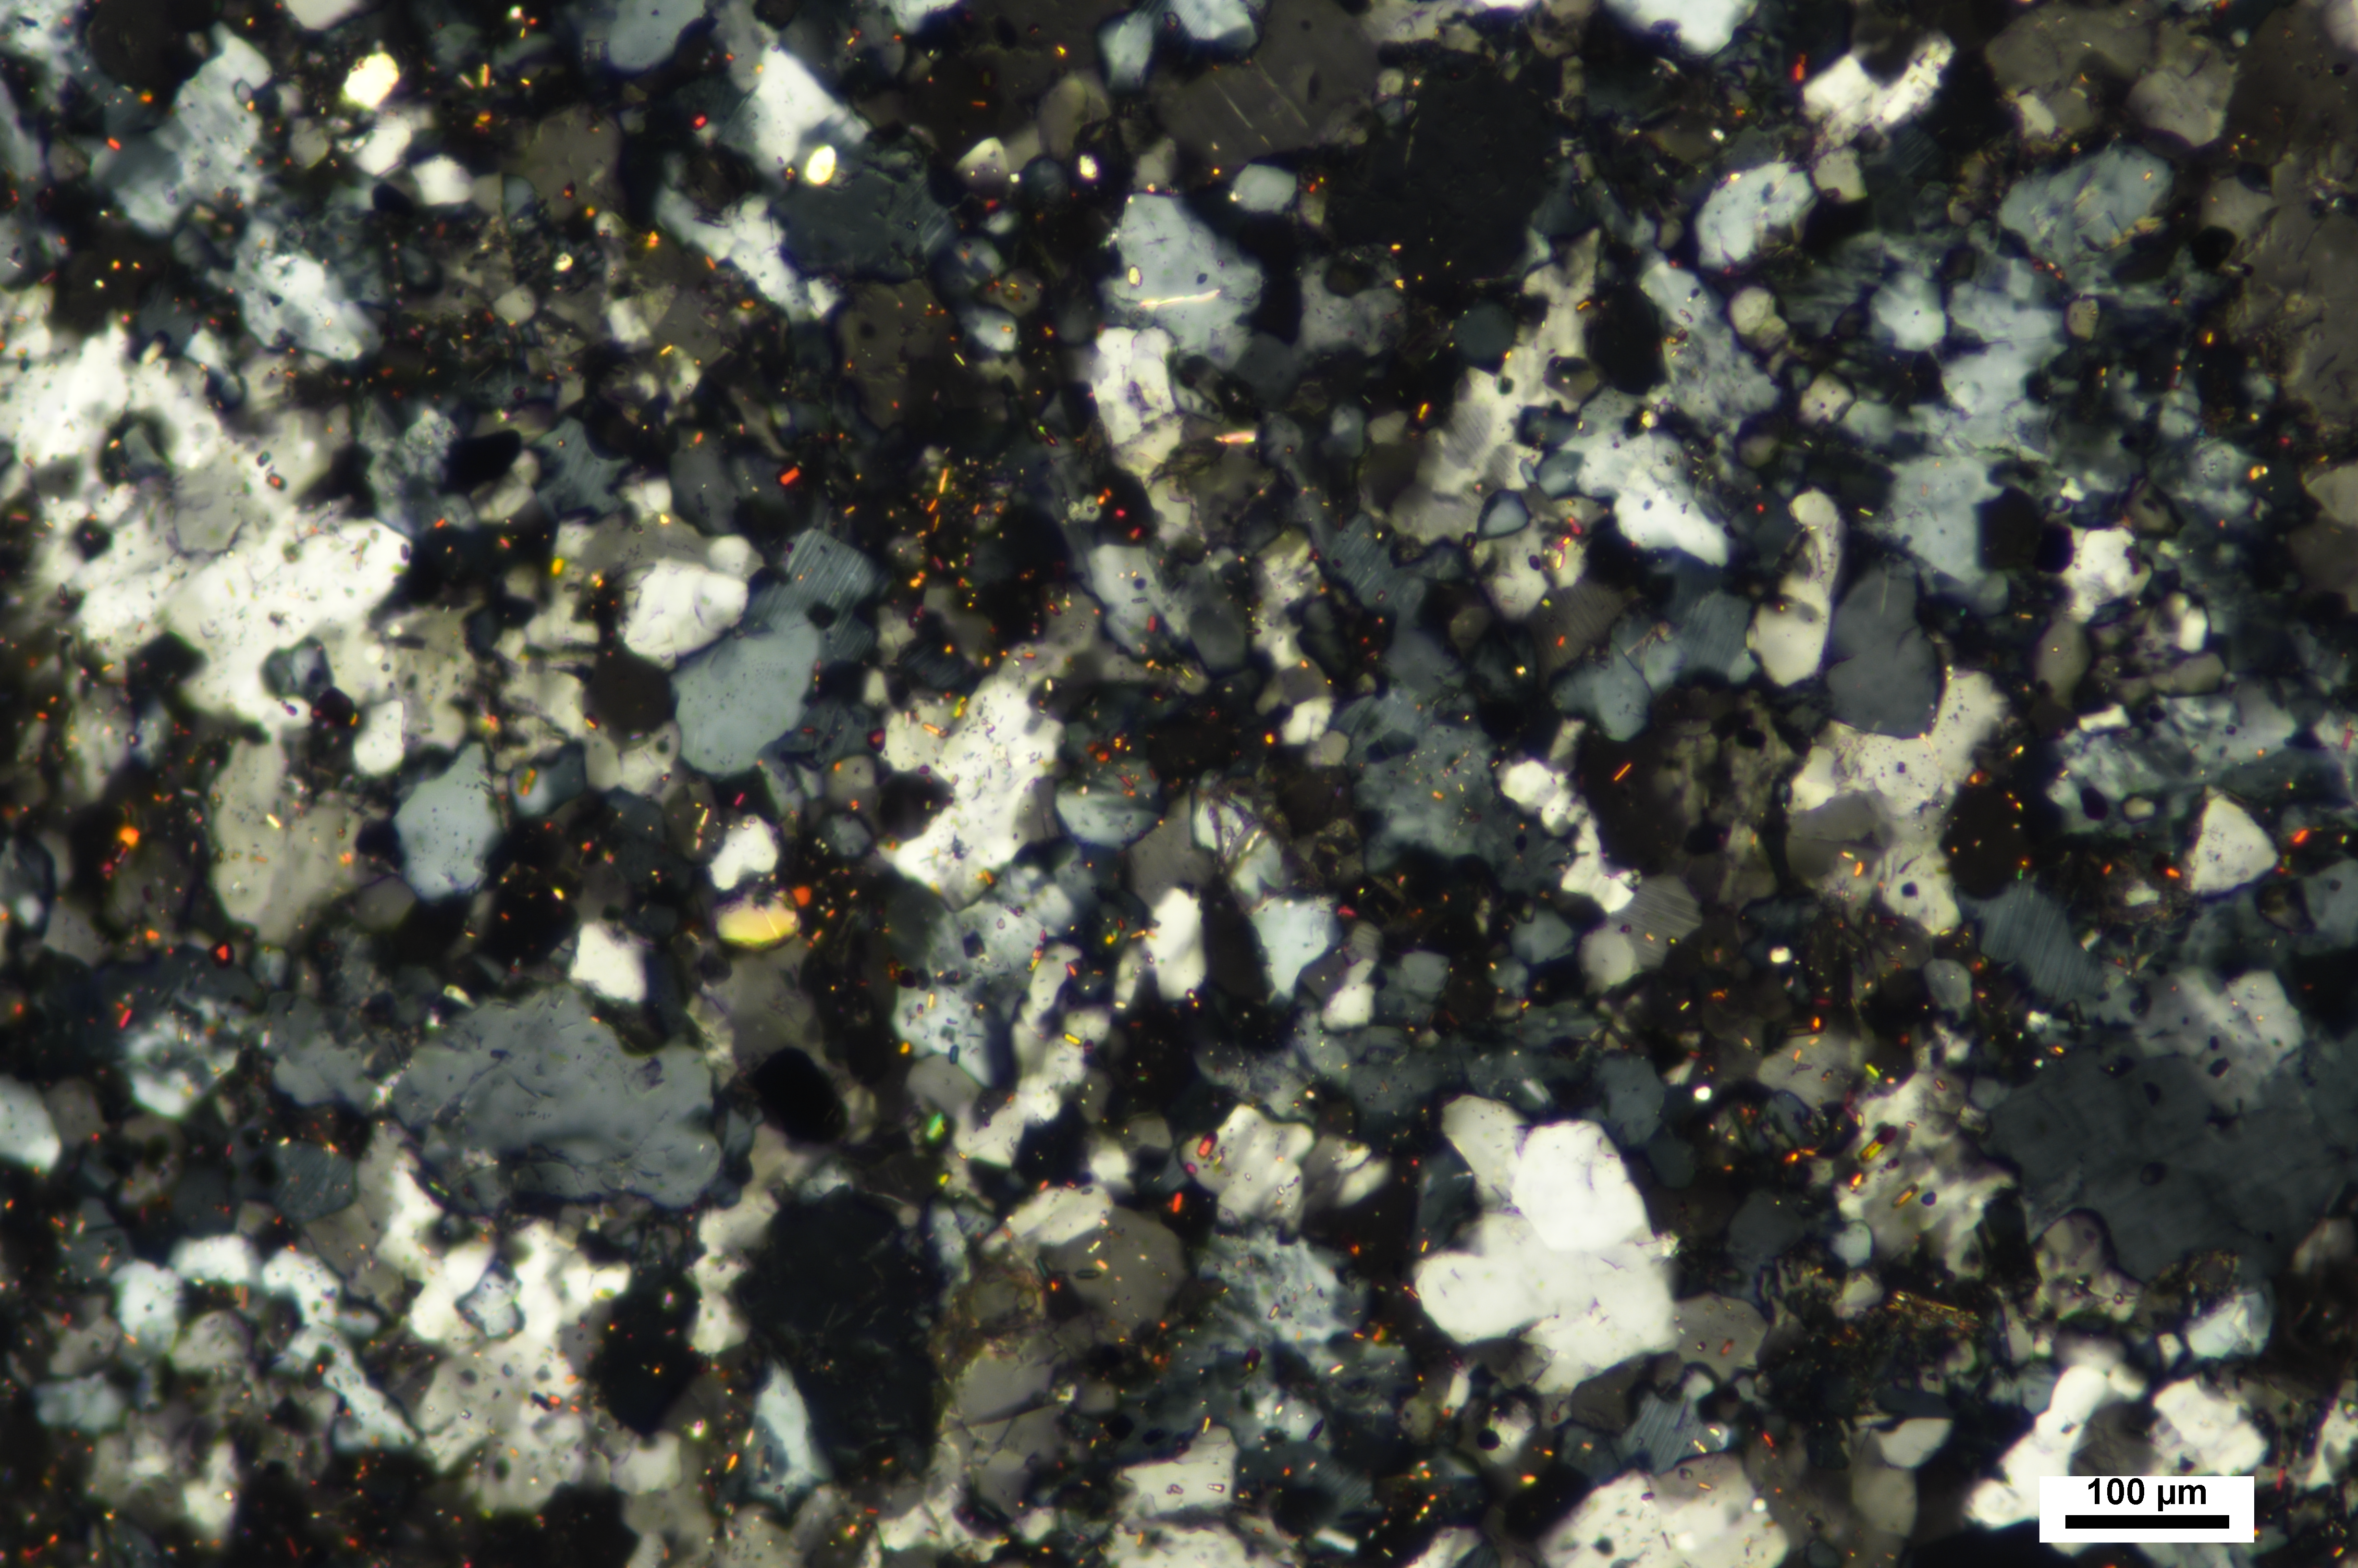
\includegraphics[width=0.7\linewidth]{figure/thin_section} 

}

\caption{Dolerite thin section under seen through a polarized microscope.}\label{fig:doleritemicro}
\end{figure}
\begin{table}[!h]

\caption{\label{tab:cherttable}Lapa do Picareiro. Identified chert types. Description is mostly based on colour patterns, following the Munsel manual of color chart (Munsel Color, 2010).}
\centering
\fontsize{9}{11}\selectfont
\begin{tabular}[t]{>{\bfseries}l>{\raggedright\arraybackslash}p{10cm}}
\toprule
Chert Type & Description\\
\midrule
RM1 & Fine grain, 2.5Y 7/6 and 6/6 (yellow and olive yellow) translucent color with opaque smoke-like patterns.\\
RM2 & Mostly 5YR 4/2 (dark reddish gray) and 4/3 (reddish brown) colouration, with 1mm 10YR 7/3 (very pale brown) dots and bigger 0.5 to 1 mm circular 10YR 7/2 (light gray) inclusions with coarser texture.\\
RM3 & Coarser texture, with veins and fog-like patterns with colour mix of 10YR 8/3, 7/3 (very pale brown), 7.5YR 7/3 (pink), 5YR 7/4 (pink) and 10YR 5/3 brown.\\
RM4 & Mostly 2.5Y 8/1 (white) with interior translucent areas.\\
RM5 & 2.5Y 6/2 (light brownish gray), closer to cortex 10YR 8/2 and 8/3 (very pale yellow) with circular 0.5 mm marks of 10YR 7/2 /(light gray) and 5Y 5/1 (gray) dots.\\
\addlinespace
RM6 & 10YR 8/3 (very pale brown) on borders, center fog-like pattern with mix of 10YR 4/2,3/3 (dark brown), 2.5Y 6/3 (light yellowish brown) and 5/1 (gray).\\
RM7 & Stripped-like ondulating pattern with several tonalities: 5YR 7/3, 8/3 (pink), 6/6 (reddish yellow), 7/1 (light gray), with certain areas with 7.5YR 7/8 (reddish yellow).\\
\bottomrule
\end{tabular}
\end{table}
\hypertarget{attribute-analysis-1}{%
\chapter{Attribute analysis}\label{attribute-analysis-1}}

\begingroup\fontsize{9}{11}\selectfont
\begin{longtable}[t]{lllll}
\caption{\label{tab:coreattributesVB1}Vale Boi - Lower 5 - core attributes frequencies.}\\
\toprule
\multicolumn{1}{c}{\textbf{Tecnological attributes}} & \multicolumn{1}{c}{\textbf{Quartz}} & \multicolumn{1}{c}{\textbf{Chert}} & \multicolumn{1}{c}{\textbf{Greywacke}} & \multicolumn{1}{c}{\textbf{Other}}\\
\midrule
\endfirsthead
\caption[]{\label{tab:coreattributesVB1}Vale Boi - Lower 5 - core attributes frequencies. \textit{(continued)}}\\
\toprule
\multicolumn{1}{c}{\textbf{Tecnological attributes}} & \multicolumn{1}{c}{\textbf{Quartz}} & \multicolumn{1}{c}{\textbf{Chert}} & \multicolumn{1}{c}{\textbf{Greywacke}} & \multicolumn{1}{c}{\textbf{Other}}\\
\midrule
\endhead
\
\endfoot
\bottomrule
\endlastfoot
CoreType, n (\%) &  &  &  & \\
Opposed & 1 (6.7) & 0 (0.0) & 0 (0.0) & 0 (0.0)\\
SinglePlat & 11 (73.3) & 8 (50.0) & 2 (100.0) & 0 (0.0)\\
SinglePrismatic & 2 (13.3) & 6 (37.5) & 0 (0.0) & 0 (0.0)\\
SinglePyramidal & 1 (6.7) & 1 (6.2) & 0 (0.0) & 1 (100.0)\\
\addlinespace
TwoSinglePlat & 0 (0.0) & 1 (6.2) & 0 (0.0) & 0 (0.0)\\
NumberCoreFaces, n (\%) &  &  &  & \\
Four & 3 (20.0) & 0 (0.0) & 0 (0.0) & 0 (0.0)\\
MoreThanFour & 0 (0.0) & 2 (12.5) & 0 (0.0) & 0 (0.0)\\
One & 4 (26.7) & 7 (43.8) & 2 (100.0) & 1 (100.0)\\
\addlinespace
Three & 3 (20.0) & 3 (18.8) & 0 (0.0) & 0 (0.0)\\
Two & 5 (33.3) & 4 (25.0) & 0 (0.0) & 0 (0.0)\\
CorePlatform, n (\%) &  &  &  & \\
Cortical & 3 (20.0) & 1 (6.2) & 2 (100.0) & 0 (0.0)\\
Faceted & 1 (6.7) & 1 (6.2) & 0 (0.0) & 0 (0.0)\\
\addlinespace
Plain & 11 (73.3) & 14 (87.5) & 0 (0.0) & 1 (100.0)\\
MainFaceCoreUse, n (\%) &  &  &  & \\
Bladelets & 1 (6.7) & 2 (12.5) & 0 (0.0) & 0 (0.0)\\
Blades & 1 (6.7) & 4 (25.0) & 0 (0.0) & 0 (0.0)\\
Flakes & 13 (86.7) & 10 (62.5) & 2 (100.0) & 0 (0.0)\\
\addlinespace
Mixed & 0 (0.0) & 0 (0.0) & 0 (0.0) & 1 (100.0)\\*
\end{longtable}
\endgroup{}

\newpage

\begingroup\fontsize{9}{11}\selectfont
\begin{longtable}[t]{lllll}
\caption{\label{tab:coreattributesVB2}Vale Boi - Upper 5/4E - core attributes frequencies.}\\
\toprule
\multicolumn{1}{c}{\textbf{Tecnological attributes}} & \multicolumn{1}{c}{\textbf{Quartz}} & \multicolumn{1}{c}{\textbf{Chert}} & \multicolumn{1}{c}{\textbf{Other}} & \multicolumn{1}{c}{\textbf{Total}}\\
\midrule
\endfirsthead
\caption[]{\label{tab:coreattributesVB2}Vale Boi - Upper 5/4E - core attributes frequencies. \textit{(continued)}}\\
\toprule
\multicolumn{1}{c}{\textbf{Tecnological attributes}} & \multicolumn{1}{c}{\textbf{Quartz}} & \multicolumn{1}{c}{\textbf{Chert}} & \multicolumn{1}{c}{\textbf{Other}} & \multicolumn{1}{c}{\textbf{Total}}\\
\midrule
\endhead
\
\endfoot
\bottomrule
\endlastfoot
CoreType, n (\%) &  &  &  & \\
Opposed & 0 (0.0) & 3 (11.1) & 0 (0.0) & 3 (5.1)\\
Other & 0 (0.0) & 3 (11.1) & 0 (0.0) & 3 (5.1)\\
SinglePlat & 21 (72.4) & 9 (33.3) & 2 (100.0) & 32 (54.2)\\
SinglePrismatic & 6 (20.7) & 3 (11.1) & 0 (0.0) & 10 (16.9)\\
\addlinespace
SinglePyramidal & 1 (3.4) & 4 (14.8) & 0 (0.0) & 5 (8.5)\\
TwoSinglePlat & 1 (3.4) & 5 (18.5) & 0 (0.0) & 6 (10.2)\\
NumberCoreFaces, n (\%) &  &  &  & \\
Four & 1 (3.4) & 2 (7.4) & 0 (0.0) & 3 (5.1)\\
MoreThanFour & 0 (0.0) & 0 (0.0) & 0 (0.0) & 1 (1.7)\\
\addlinespace
One & 14 (48.3) & 12 (44.4) & 2 (100.0) & 28 (47.5)\\
Three & 2 (6.9) & 4 (14.8) & 0 (0.0) & 6 (10.2)\\
Two & 12 (41.4) & 9 (33.3) & 0 (0.0) & 21 (35.6)\\
CorePlatform, n (\%) &  &  &  & \\
Cortical & 9 (31.0) & 1 (3.7) & 1 (50.0) & 11 (18.6)\\
\addlinespace
Crushed & 1 (3.4) & 2 (7.4) & 0 (0.0) & 3 (5.1)\\
Dihedral & 0 (0.0) & 2 (7.4) & 0 (0.0) & 2 (3.4)\\
Faceted & 1 (3.4) & 5 (18.5) & 0 (0.0) & 6 (10.2)\\
Other & 0 (0.0) & 2 (7.4) & 0 (0.0) & 2 (3.4)\\
Plain & 18 (62.1) & 15 (55.6) & 1 (50.0) & 35 (59.3)\\
\addlinespace
MainFaceCoreUse, n (\%) &  &  &  & \\
Bladelets & 3 (10.3) & 3 (11.1) & 0 (0.0) & 6 (10.2)\\
Blades & 2 (6.9) & 4 (14.8) & 0 (0.0) & 6 (10.2)\\
Flakes & 20 (69.0) & 16 (59.3) & 2 (100.0) & 39 (66.1)\\
Mixed & 4 (13.8) & 4 (14.8) & 0 (0.0) & 8 (13.6)\\*
\end{longtable}
\endgroup{}

\newpage
\begin{table}[!h]

\caption{\label{tab:coremetricsVB1}Vale Boi - Lower 5 - mean and standard deviation of core measurements (in mm).}
\centering
\resizebox{\linewidth}{!}{
\fontsize{9}{11}\selectfont
\begin{tabular}[t]{llllll}
\toprule
\multicolumn{1}{c}{\textbf{Core metrics}} & \multicolumn{1}{c}{\textbf{Quartz}} & \multicolumn{1}{c}{\textbf{Chert}} & \multicolumn{1}{c}{\textbf{Greywacke}} & \multicolumn{1}{c}{\textbf{Other}} & \multicolumn{1}{c}{\textbf{Total}}\\
\midrule
MedWidth, M (SD) & 31.6 (14.0) & 30.3 (15.2) & 59.7 (28.1) & 41.0 (NA) & 32.8 (16.7)\\
Length, M (SD) & 26.6 (7.2) & 29.1 (12.9) & 32.4 (10.5) & 36.3 (NA) & 28.7 (10.5)\\
Thickness, M (SD) & 23.4 (11.8) & 22.8 (6.6) & 36.1 (8.0) & 32.6 (NA) & 24.1 (9.5)\\
PlatformWidth, M (SD) & 32.1 (13.2) & 29.2 (11.6) & 64.6 (26.3) & 35.6 (NA) & 32.6 (15.5)\\
PlatformThickness, M (SD) & 22.1 (11.3) & 21.4 (7.0) & 40.3 (9.4) & 23.9 (NA) & 22.9 (9.9)\\
\addlinespace
MainFacePlatformAngle, M (SD) & 68.1 (32.8) & 56.2 (40.2) & 56.5 (52.2) & 83.1 (NA) & 60.2 (38.0)\\
Weight, M (SD) & 35.0 (44.7) & 35.0 (64.4) & 107.5 (80.0) & 84.8 (NA) & 40.7 (58.6)\\
\bottomrule
\end{tabular}}
\end{table}
\begin{table}[!h]

\caption{\label{tab:coremetricsVB2}Vale Boi - Upper 5/4E - mean and standard deviation of core measurements (in mm).}
\centering
\resizebox{\linewidth}{!}{
\fontsize{9}{11}\selectfont
\begin{tabular}[t]{llllll}
\toprule
\multicolumn{1}{c}{\textbf{Core metrics}} & \multicolumn{1}{c}{\textbf{Quartz}} & \multicolumn{1}{c}{\textbf{Chert}} & \multicolumn{1}{c}{\textbf{Greywacke}} & \multicolumn{1}{c}{\textbf{Other}} & \multicolumn{1}{c}{\textbf{Total}}\\
\midrule
MedWidth, M (SD) & 33.4 (13.0) & 26.5 (8.7) & 18.5 (NA) & 51.4 (6.8) & 29.9 (11.7)\\
Length, M (SD) & 25.8 (10.2) & 26.5 (8.9) & 33.9 (NA) & 36.9 (26.3) & 26.6 (9.9)\\
Thickness, M (SD) & 27.0 (9.9) & 21.6 (10.0) & 18.1 (NA) & 32.6 (9.4) & 24.1 (10.3)\\
PlatformWidth, M (SD) & 34.4 (13.1) & 25.9 (9.0) & 17.5 (NA) & 43.1 (16.7) & 29.8 (11.9)\\
PlatformThickness, M (SD) & 26.8 (10.3) & 20.1 (9.5) & 16.1 (NA) & 19.5 (2.5) & 22.8 (10.2)\\
\addlinespace
MainFacePlatformAngle, M (SD) & 70.4 (26.0) & 52.2 (42.5) & 86.7 (NA) & 89.8 (18.3) & 61.2 (37.0)\\
Weight, M (SD) & 41.2 (50.9) & 20.8 (15.1) & 14.7 (NA) & 99.8 (79.2) & 31.2 (38.6)\\
\bottomrule
\end{tabular}}
\end{table}
\newpage

\begingroup\fontsize{9}{11}\selectfont
\begin{longtable}[t]{>{\raggedright\arraybackslash}p{1cm}>{\raggedright\arraybackslash}p{1cm}>{\raggedright\arraybackslash}p{1cm}>{\raggedright\arraybackslash}p{1cm}>{\raggedright\arraybackslash}p{1cm}>{\raggedright\arraybackslash}p{1cm}>{\raggedright\arraybackslash}p{1cm}>{\raggedright\arraybackslash}p{1cm}}
\caption{\label{tab:flakeattributeVB1}Vale Boi - Lower 5 - flake attributes frequencies.}\\
\toprule
\multicolumn{1}{c}{\textbf{Attributes}} & \multicolumn{1}{c}{\textbf{Quartz}} & \multicolumn{1}{c}{\textbf{Chert}} & \multicolumn{1}{c}{\textbf{Greywacke}} & \multicolumn{1}{c}{\textbf{Dolerite}} & \multicolumn{1}{c}{\textbf{Chalcedony}} & \multicolumn{1}{c}{\textbf{Other}} & \multicolumn{1}{c}{\textbf{Total}}\\
\midrule
\endfirsthead
\caption[]{\label{tab:flakeattributeVB1}Vale Boi - Lower 5 - flake attributes frequencies. \textit{(continued)}}\\
\toprule
\multicolumn{1}{c}{\textbf{Attributes}} & \multicolumn{1}{c}{\textbf{Quartz}} & \multicolumn{1}{c}{\textbf{Chert}} & \multicolumn{1}{c}{\textbf{Greywacke}} & \multicolumn{1}{c}{\textbf{Dolerite}} & \multicolumn{1}{c}{\textbf{Chalcedony}} & \multicolumn{1}{c}{\textbf{Other}} & \multicolumn{1}{c}{\textbf{Total}}\\
\midrule
\endhead
\
\endfoot
\bottomrule
\endlastfoot
CrossSection, n (\%) &  &  &  &  &  &  & \\
Irregular & 118 (49.8) & 50 (35.7) & 12 (31.6) & 1 (33.3) & 2 (40.0) & 2 (50.0) & 185 (43.3)\\
Lenticular & 24 (10.1) & 32 (22.9) & 7 (18.4) & 0 (0.0) & 0 (0.0) & 1 (25.0) & 64 (15.0)\\
Other & 5 (2.1) & 3 (2.1) & 0 (0.0) & 0 (0.0) & 0 (0.0) & 0 (0.0) & 8 (1.9)\\
Quadrangular & 13 (5.5) & 3 (2.1) & 3 (7.9) & 0 (0.0) & 0 (0.0) & 1 (25.0) & 20 (4.7)\\
\addlinespace
Trapezoidal & 11 (4.6) & 5 (3.6) & 4 (10.5) & 0 (0.0) & 0 (0.0) & 0 (0.0) & 20 (4.7)\\
Triangular & 66 (27.8) & 47 (33.6) & 12 (31.6) & 2 (66.7) & 3 (60.0) & 0 (0.0) & 130 (30.4)\\
BlankShape, n (\%) &  &  &  &  &  &  & \\
Circular & 9 (3.8) & 4 (2.9) & 1 (2.6) & 0 (0.0) & 0 (0.0) & 1 (25.0) & 15 (3.5)\\
Convergent & 60 (25.3) & 20 (14.3) & 8 (21.1) & 1 (33.3) & 1 (20.0) & 0 (0.0) & 90 (21.1)\\
\addlinespace
Dejete & 4 (1.7) & 5 (3.6) & 0 (0.0) & 0 (0.0) & 0 (0.0) & 0 (0.0) & 9 (2.1)\\
Divergent & 9 (3.8) & 19 (13.6) & 2 (5.3) & 0 (0.0) & 1 (20.0) & 1 (25.0) & 32 (7.5)\\
Irregular & 108 (45.6) & 68 (48.6) & 20 (52.6) & 0 (0.0) & 3 (60.0) & 0 (0.0) & 199 (46.6)\\
Parallel & 47 (19.8) & 24 (17.1) & 7 (18.4) & 2 (66.7) & 0 (0.0) & 2 (50.0) & 82 (19.2)\\
Profile, n (\%) &  &  &  &  &  &  & \\
\addlinespace
Curved & 32 (13.5) & 62 (44.3) & 7 (18.4) & 1 (33.3) & 0 (0.0) & 3 (75.0) & 105 (24.6)\\
Irregular & 47 (19.8) & 14 (10.0) & 9 (23.7) & 0 (0.0) & 2 (40.0) & 0 (0.0) & 72 (16.9)\\
Straight & 154 (65.0) & 60 (42.9) & 21 (55.3) & 2 (66.7) & 2 (40.0) & 1 (25.0) & 240 (56.2)\\
Twisted & 4 (1.7) & 4 (2.9) & 1 (2.6) & 0 (0.0) & 1 (20.0) & 0 (0.0) & 10 (2.3)\\
BlankTip, n (\%) &  &  &  &  &  &  & \\
\addlinespace
Feather & 65 (27.4) & 68 (48.6) & 15 (39.5) & 0 (0.0) & 2 (40.0) & 1 (25.0) & 151 (35.4)\\
Hinge & 107 (45.1) & 28 (20.0) & 10 (26.3) & 2 (66.7) & 1 (20.0) & 1 (25.0) & 149 (34.9)\\
Overshoot & 1 (0.4) & 4 (2.9) & 0 (0.0) & 0 (0.0) & 0 (0.0) & 0 (0.0) & 5 (1.2)\\
Pointed & 31 (13.1) & 9 (6.4) & 2 (5.3) & 0 (0.0) & 0 (0.0) & 0 (0.0) & 42 (9.8)\\
Step & 33 (13.9) & 31 (22.1) & 11 (28.9) & 1 (33.3) & 2 (40.0) & 2 (50.0) & 80 (18.7)\\
\addlinespace
PlatformType, n (\%) &  &  &  &  &  &  & \\
Crushed & 79 (33.3) & 21 (15.0) & 2 (5.3) & 1 (33.3) & 2 (40.0) & 0 (0.0) & 105 (24.6)\\
Dihedral & 2 (0.8) & 6 (4.3) & 0 (0.0) & 0 (0.0) & 0 (0.0) & 0 (0.0) & 8 (1.9)\\
Faceted & 0 (0.0) & 2 (1.4) & 0 (0.0) & 0 (0.0) & 0 (0.0) & 0 (0.0) & 2 (0.5)\\
Linear & 0 (0.0) & 5 (3.6) & 1 (2.6) & 0 (0.0) & 0 (0.0) & 0 (0.0) & 6 (1.4)\\
\addlinespace
Other & 2 (0.8) & 0 (0.0) & 1 (2.6) & 0 (0.0) & 0 (0.0) & 0 (0.0) & 3 (0.7)\\
Plain & 154 (65.0) & 97 (69.3) & 34 (89.5) & 2 (66.7) & 3 (60.0) & 3 (75.0) & 293 (68.6)\\
Winged & 0 (0.0) & 9 (6.4) & 0 (0.0) & 0 (0.0) & 0 (0.0) & 1 (25.0) & 10 (2.3)\\
PlatformCortex, n (\%) &  &  &  &  &  &  & \\
No & 233 (98.3) & 121 (86.4) & 34 (89.5) & 3 (100.0) & 5 (100.0) & 4 (100.0) & 400 (93.7)\\
\addlinespace
YesComplete & 3 (1.3) & 15 (10.7) & 4 (10.5) & 0 (0.0) & 0 (0.0) & 0 (0.0) & 22 (5.2)\\
YesPartial & 1 (0.4) & 4 (2.9) & 0 (0.0) & 0 (0.0) & 0 (0.0) & 0 (0.0) & 5 (1.2)\\
ScarCount, n (\%) &  &  &  &  &  &  & \\
0 & 2 (0.8) & 2 (1.4) & 2 (5.3) & 0 (0.0) & 0 (0.0) & 0 (0.0) & 6 (1.4)\\
1 & 89 (37.6) & 39 (27.9) & 17 (44.7) & 1 (33.3) & 1 (20.0) & 3 (75.0) & 150 (35.1)\\
\addlinespace
2 & 100 (42.2) & 49 (35.0) & 11 (28.9) & 1 (33.3) & 3 (60.0) & 1 (25.0) & 165 (38.6)\\
3 & 38 (16.0) & 32 (22.9) & 4 (10.5) & 1 (33.3) & 0 (0.0) & 0 (0.0) & 75 (17.6)\\
4 & 7 (3.0) & 12 (8.6) & 3 (7.9) & 0 (0.0) & 1 (20.0) & 0 (0.0) & 23 (5.4)\\
5 & 0 (0.0) & 5 (3.6) & 0 (0.0) & 0 (0.0) & 0 (0.0) & 0 (0.0) & 5 (1.2)\\
6 & 1 (0.4) & 0 (0.0) & 0 (0.0) & 0 (0.0) & 0 (0.0) & 0 (0.0) & 1 (0.2)\\
\addlinespace
7 & 0 (0.0) & 1 (0.7) & 0 (0.0) & 0 (0.0) & 0 (0.0) & 0 (0.0) & 1 (0.2)\\
8 & 0 (0.0) & 0 (0.0) & 1 (2.6) & 0 (0.0) & 0 (0.0) & 0 (0.0) & 1 (0.2)\\
Cortex, n (\%) &  &  &  &  &  &  & \\
0\% & 227 (95.8) & 115 (82.1) & 31 (81.6) & 3 (100.0) & 5 (100.0) & 4 (100.0) & 385 (90.2)\\
1-30\% & 4 (1.7) & 13 (9.3) & 0 (0.0) & 0 (0.0) & 0 (0.0) & 0 (0.0) & 17 (4.0)\\
\addlinespace
100\% & 2 (0.8) & 2 (1.4) & 2 (5.3) & 0 (0.0) & 0 (0.0) & 0 (0.0) & 6 (1.4)\\
31-60\% & 3 (1.3) & 6 (4.3) & 3 (7.9) & 0 (0.0) & 0 (0.0) & 0 (0.0) & 12 (2.8)\\
61-99\% & 1 (0.4) & 4 (2.9) & 2 (5.3) & 0 (0.0) & 0 (0.0) & 0 (0.0) & 7 (1.6)\\*
\end{longtable}
\endgroup{}

\newpage

\begingroup\fontsize{9}{11}\selectfont
\begin{longtable}[t]{>{\raggedright\arraybackslash}p{1cm}>{\raggedright\arraybackslash}p{1cm}>{\raggedright\arraybackslash}p{1cm}>{\raggedright\arraybackslash}p{1cm}>{\raggedright\arraybackslash}p{1cm}>{\raggedright\arraybackslash}p{1cm}>{\raggedright\arraybackslash}p{1cm}>{\raggedright\arraybackslash}p{1cm}}
\caption{\label{tab:flakeattributeVB2}Vale Boi - Upper 5/4E - flake attributes frequencies.}\\
\toprule
\multicolumn{1}{c}{\textbf{Attributes}} & \multicolumn{1}{c}{\textbf{Quartz}} & \multicolumn{1}{c}{\textbf{Chert}} & \multicolumn{1}{c}{\textbf{Greywacke}} & \multicolumn{1}{c}{\textbf{Dolerite}} & \multicolumn{1}{c}{\textbf{Chalcedony}} & \multicolumn{1}{c}{\textbf{Other}} & \multicolumn{1}{c}{\textbf{Total}}\\
\midrule
\endfirsthead
\caption[]{\label{tab:flakeattributeVB2}Vale Boi - Upper 5/4E - flake attributes frequencies. \textit{(continued)}}\\
\toprule
\multicolumn{1}{c}{\textbf{Attributes}} & \multicolumn{1}{c}{\textbf{Quartz}} & \multicolumn{1}{c}{\textbf{Chert}} & \multicolumn{1}{c}{\textbf{Greywacke}} & \multicolumn{1}{c}{\textbf{Dolerite}} & \multicolumn{1}{c}{\textbf{Chalcedony}} & \multicolumn{1}{c}{\textbf{Other}} & \multicolumn{1}{c}{\textbf{Total}}\\
\midrule
\endhead
\
\endfoot
\bottomrule
\endlastfoot
CrossSection, n (\%) &  &  &  &  &  &  & \\
Irregular & 191 (49.4) & 121 (36.4) & 30 (39.5) & 5 (38.5) & 6 (42.9) & 1 (16.7) & 354 (42.8)\\
Lenticular & 44 (11.4) & 45 (13.6) & 19 (25.0) & 1 (7.7) & 2 (14.3) & 1 (16.7) & 112 (13.5)\\
Other & 6 (1.6) & 7 (2.1) & 2 (2.6) & 0 (0.0) & 0 (0.0) & 0 (0.0) & 15 (1.8)\\
Quadrangular & 14 (3.6) & 4 (1.2) & 1 (1.3) & 0 (0.0) & 0 (0.0) & 0 (0.0) & 19 (2.3)\\
\addlinespace
Trapezoidal & 12 (3.1) & 24 (7.2) & 2 (2.6) & 3 (23.1) & 2 (14.3) & 0 (0.0) & 43 (5.2)\\
Triangular & 120 (31.0) & 131 (39.5) & 22 (28.9) & 4 (30.8) & 4 (28.6) & 4 (66.7) & 285 (34.4)\\
BlankShape, n (\%) &  &  &  &  &  &  & \\
Circular & 16 (4.1) & 7 (2.1) & 2 (2.6) & 1 (7.7) & 1 (7.1) & 0 (0.0) & 27 (3.3)\\
Convergent & 113 (29.2) & 67 (20.2) & 13 (17.1) & 1 (7.7) & 3 (21.4) & 0 (0.0) & 197 (23.8)\\
\addlinespace
Dejete & 6 (1.6) & 15 (4.5) & 8 (10.5) & 0 (0.0) & 0 (0.0) & 0 (0.0) & 29 (3.5)\\
Divergent & 32 (8.3) & 55 (16.6) & 6 (7.9) & 2 (15.4) & 2 (14.3) & 0 (0.0) & 97 (11.7)\\
Irregular & 111 (28.7) & 118 (35.5) & 41 (53.9) & 9 (69.2) & 4 (28.6) & 5 (83.3) & 288 (34.8)\\
Other & 1 (0.3) & 0 (0.0) & 0 (0.0) & 0 (0.0) & 0 (0.0) & 0 (0.0) & 1 (0.1)\\
Parallel & 108 (27.9) & 70 (21.1) & 6 (7.9) & 0 (0.0) & 4 (28.6) & 1 (16.7) & 189 (22.8)\\
\addlinespace
Profile, n (\%) &  &  &  &  &  &  & \\
Curved & 75 (19.4) & 146 (44.0) & 24 (31.6) & 6 (46.2) & 6 (42.9) & 4 (66.7) & 261 (31.5)\\
Irregular & 60 (15.5) & 24 (7.2) & 10 (13.2) & 1 (7.7) & 2 (14.3) & 0 (0.0) & 97 (11.7)\\
Straight & 246 (63.6) & 157 (47.3) & 42 (55.3) & 5 (38.5) & 6 (42.9) & 2 (33.3) & 458 (55.3)\\
Twisted & 6 (1.6) & 5 (1.5) & 0 (0.0) & 1 (7.7) & 0 (0.0) & 0 (0.0) & 12 (1.4)\\
\addlinespace
BlankTip, n (\%) &  &  &  &  &  &  & \\
Feather & 76 (19.6) & 139 (41.9) & 34 (44.7) & 6 (46.2) & 9 (64.3) & 3 (50.0) & 267 (32.2)\\
Hinge & 220 (56.8) & 64 (19.3) & 22 (28.9) & 2 (15.4) & 1 (7.1) & 2 (33.3) & 311 (37.6)\\
Overshoot & 3 (0.8) & 8 (2.4) & 0 (0.0) & 0 (0.0) & 0 (0.0) & 0 (0.0) & 11 (1.3)\\
Pointed & 49 (12.7) & 29 (8.7) & 8 (10.5) & 0 (0.0) & 2 (14.3) & 0 (0.0) & 88 (10.6)\\
\addlinespace
Step & 39 (10.1) & 92 (27.7) & 12 (15.8) & 5 (38.5) & 2 (14.3) & 1 (16.7) & 151 (18.2)\\
PlatformType, n (\%) &  &  &  &  &  &  & \\
Crushed & 139 (35.9) & 53 (16.0) & 5 (6.6) & 2 (15.4) & 2 (14.3) & 0 (0.0) & 201 (24.3)\\
Dihedral & 2 (0.5) & 23 (6.9) & 1 (1.3) & 1 (7.7) & 3 (21.4) & 0 (0.0) & 30 (3.6)\\
Faceted & 0 (0.0) & 8 (2.4) & 1 (1.3) & 0 (0.0) & 0 (0.0) & 0 (0.0) & 9 (1.1)\\
\addlinespace
Linear & 2 (0.5) & 10 (3.0) & 3 (3.9) & 1 (7.7) & 0 (0.0) & 0 (0.0) & 16 (1.9)\\
Other & 0 (0.0) & 1 (0.3) & 0 (0.0) & 0 (0.0) & 0 (0.0) & 0 (0.0) & 1 (0.1)\\
Plain & 243 (62.8) & 217 (65.4) & 66 (86.8) & 9 (69.2) & 7 (50.0) & 6 (100.0) & 548 (66.2)\\
Winged & 1 (0.3) & 20 (6.0) & 0 (0.0) & 0 (0.0) & 2 (14.3) & 0 (0.0) & 23 (2.8)\\
PlatformCortex, n (\%) &  &  &  &  &  &  & \\
\addlinespace
No & 377 (97.4) & 270 (81.3) & 65 (85.5) & 12 (92.3) & 14 (100.0) & 5 (83.3) & 743 (89.7)\\
YesComplete & 6 (1.6) & 35 (10.5) & 11 (14.5) & 1 (7.7) & 0 (0.0) & 1 (16.7) & 54 (6.5)\\
YesPartial & 4 (1.0) & 27 (8.1) & 0 (0.0) & 0 (0.0) & 0 (0.0) & 0 (0.0) & 31 (3.7)\\
ScarCount, n (\%) &  &  &  &  &  &  & \\
0 & 5 (1.3) & 16 (4.8) & 2 (2.6) & 0 (0.0) & 0 (0.0) & 1 (16.7) & 24 (2.9)\\
\addlinespace
1 & 156 (40.3) & 78 (23.5) & 25 (32.9) & 3 (23.1) & 5 (35.7) & 0 (0.0) & 267 (32.2)\\
2 & 160 (41.3) & 125 (37.7) & 30 (39.5) & 6 (46.2) & 4 (28.6) & 3 (50.0) & 328 (39.6)\\
3 & 60 (15.5) & 79 (23.8) & 14 (18.4) & 4 (30.8) & 2 (14.3) & 2 (33.3) & 161 (19.4)\\
4 & 5 (1.3) & 26 (7.8) & 2 (2.6) & 0 (0.0) & 1 (7.1) & 0 (0.0) & 34 (4.1)\\
5 & 1 (0.3) & 5 (1.5) & 2 (2.6) & 0 (0.0) & 0 (0.0) & 0 (0.0) & 8 (1.0)\\
\addlinespace
6 & 0 (0.0) & 3 (0.9) & 1 (1.3) & 0 (0.0) & 1 (7.1) & 0 (0.0) & 5 (0.6)\\
8 & 0 (0.0) & 0 (0.0) & 0 (0.0) & 0 (0.0) & 1 (7.1) & 0 (0.0) & 1 (0.1)\\
Cortex, n (\%) &  &  &  &  &  &  & \\
0\% & 369 (95.3) & 231 (69.6) & 66 (86.8) & 11 (84.6) & 14 (100.0) & 4 (66.7) & 695 (83.9)\\
1-30\% & 5 (1.3) & 55 (16.6) & 5 (6.6) & 1 (7.7) & 0 (0.0) & 1 (16.7) & 67 (8.1)\\
\addlinespace
100\% & 5 (1.3) & 16 (4.8) & 2 (2.6) & 0 (0.0) & 0 (0.0) & 1 (16.7) & 24 (2.9)\\
31-60\% & 7 (1.8) & 11 (3.3) & 1 (1.3) & 1 (7.7) & 0 (0.0) & 0 (0.0) & 20 (2.4)\\
61-99\% & 1 (0.3) & 19 (5.7) & 2 (2.6) & 0 (0.0) & 0 (0.0) & 0 (0.0) & 22 (2.7)\\*
\end{longtable}
\endgroup{}

\newpage
\begin{table}[!h]

\caption{\label{tab:flakemetricsVB1}Vale Boi - Lower 5 - mean and standard deviation of flake measurements (in mm).}
\centering
\resizebox{\linewidth}{!}{
\fontsize{9}{11}\selectfont
\begin{tabular}[t]{llllllll}
\toprule
\multicolumn{1}{c}{\textbf{Measurements}} & \multicolumn{1}{c}{\textbf{Quartz}} & \multicolumn{1}{c}{\textbf{Chert}} & \multicolumn{1}{c}{\textbf{Greywacke}} & \multicolumn{1}{c}{\textbf{Dolerite}} & \multicolumn{1}{c}{\textbf{Chalcedony}} & \multicolumn{1}{c}{\textbf{Other}} & \multicolumn{1}{c}{\textbf{Total}}\\
\midrule
MedWidth, M (SD) & 18.4 (6.8) & 16.6 (6.3) & 28.8 (13.5) & 14.7 (3.9) & 15.0 (5.7) & 23.0 (3.5) & 18.7 (8.1)\\
Length, M (SD) & 23.0 (7.6) & 19.4 (7.3) & 32.9 (13.5) & 18.0 (5.0) & 20.6 (10.2) & 26.3 (7.4) & 22.7 (8.9)\\
Thickness, M (SD) & 8.9 (3.8) & 5.5 (2.6) & 10.9 (6.0) & 5.5 (1.3) & 6.6 (3.5) & 6.6 (3.0) & 7.9 (4.1)\\
PlatformWidth, M (SD) & 15.2 (7.4) & 10.9 (5.6) & 21.9 (12.1) & 11.1 (3.4) & 8.8 (4.7) & 12.6 (5.1) & 14.3 (7.9)\\
PlatformThickness, M (SD) & 7.84 (4.20) & 4.58 (2.44) & 9.84 (5.07) & 4.86 (1.17) & 4.45 (2.87) & 5.27 (3.46) & 6.86 (4.16)\\
\bottomrule
\end{tabular}}
\end{table}
\begin{table}[!h]

\caption{\label{tab:flakemetricsVB2}Vale Boi - Upper 5/4E - mean and standard deviation of flake measurements (in mm).}
\centering
\resizebox{\linewidth}{!}{
\fontsize{9}{11}\selectfont
\begin{tabular}[t]{llllllll}
\toprule
\multicolumn{1}{c}{\textbf{Measurements}} & \multicolumn{1}{c}{\textbf{Quartz}} & \multicolumn{1}{c}{\textbf{Chert}} & \multicolumn{1}{c}{\textbf{Greywacke}} & \multicolumn{1}{c}{\textbf{Dolerite}} & \multicolumn{1}{c}{\textbf{Chalcedony}} & \multicolumn{1}{c}{\textbf{Other}} & \multicolumn{1}{c}{\textbf{Total}}\\
\midrule
MedWidth, M (SD) & 18.1 (7.2) & 16.7 (6.2) & 25.9 (10.8) & 21.1 (7.1) & 17.7 (5.1) & 25.6 (11.0) & 18.3 (7.7)\\
Length, M (SD) & 23.2 (8.0) & 21.0 (7.3) & 28.6 (11.1) & 23.1 (8.0) & 21.1 (8.4) & 39.3 (13.7) & 22.9 (8.5)\\
Thickness, M (SD) & 8.7 (3.5) & 5.9 (3.0) & 9.2 (4.5) & 6.1 (2.9) & 6.3 (2.1) & 10.6 (2.8) & 7.6 (3.7)\\
PlatformWidth, M (SD) & 15.3 (7.7) & 11.4 (5.1) & 20.3 (9.3) & 17.7 (10.5) & 13.3 (4.7) & 16.4 (5.5) & 14.2 (7.4)\\
PlatformThickness, M (SD) & 7.56 (3.71) & 4.93 (2.74) & 7.83 (4.24) & 5.45 (3.09) & 5.43 (2.11) & 8.23 (3.10) & 6.47 (3.62)\\
\bottomrule
\end{tabular}}
\end{table}
\newpage

\begingroup\fontsize{9}{11}\selectfont
\begin{longtable}[t]{>{\raggedright\arraybackslash}p{0.8cm}>{\raggedright\arraybackslash}p{0.8cm}>{\raggedright\arraybackslash}p{0.8cm}>{\raggedright\arraybackslash}p{0.8cm}>{\raggedright\arraybackslash}p{0.8cm}>{\raggedright\arraybackslash}p{0.8cm}}
\caption{\label{tab:elongtableVB1}Vale Boi - Lower 5 - elongated products attributes frequencies.}\\
\toprule
\multicolumn{1}{c}{\textbf{Attributes}} & \multicolumn{1}{c}{\textbf{Quartz}} & \multicolumn{1}{c}{\textbf{Chert}} & \multicolumn{1}{c}{\textbf{Greywacke}} & \multicolumn{1}{c}{\textbf{Chalcedony}} & \multicolumn{1}{c}{\textbf{Total}}\\
\midrule
\endfirsthead
\caption[]{\label{tab:elongtableVB1}Vale Boi - Lower 5 - elongated products attributes frequencies. \textit{(continued)}}\\
\toprule
\multicolumn{1}{c}{\textbf{Attributes}} & \multicolumn{1}{c}{\textbf{Quartz}} & \multicolumn{1}{c}{\textbf{Chert}} & \multicolumn{1}{c}{\textbf{Greywacke}} & \multicolumn{1}{c}{\textbf{Chalcedony}} & \multicolumn{1}{c}{\textbf{Total}}\\
\midrule
\endhead
\
\endfoot
\bottomrule
\endlastfoot
CrossSection, n (\%) &  &  &  &  & \\
Irregular & 12 (27.3) & 2 (6.5) & 2 (33.3) & 1 (100.0) & 17 (20.7)\\
Lenticular & 2 (4.5) & 2 (6.5) & 0 (0.0) & 0 (0.0) & 4 (4.9)\\
Quadrangular & 3 (6.8) & 1 (3.2) & 1 (16.7) & 0 (0.0) & 5 (6.1)\\
Trapezoidal & 1 (2.3) & 2 (6.5) & 1 (16.7) & 0 (0.0) & 4 (4.9)\\
\addlinespace
Triangular & 26 (59.1) & 24 (77.4) & 2 (33.3) & 0 (0.0) & 52 (63.4)\\
BlankShape, n (\%) &  &  &  &  & \\
Convergent & 11 (25.0) & 16 (51.6) & 3 (50.0) & 0 (0.0) & 30 (36.6)\\
Dejete & 0 (0.0) & 1 (3.2) & 1 (16.7) & 0 (0.0) & 2 (2.4)\\
Divergent & 1 (2.3) & 1 (3.2) & 0 (0.0) & 0 (0.0) & 2 (2.4)\\
\addlinespace
Irregular & 4 (9.1) & 4 (12.9) & 1 (16.7) & 1 (100.0) & 10 (12.2)\\
Parallel & 28 (63.6) & 9 (29.0) & 1 (16.7) & 0 (0.0) & 38 (46.3)\\
Profile, n (\%) &  &  &  &  & \\
Curved & 10 (22.7) & 12 (38.7) & 1 (16.7) & 0 (0.0) & 23 (28.0)\\
Irregular & 1 (2.3) & 2 (6.5) & 0 (0.0) & 0 (0.0) & 3 (3.7)\\
\addlinespace
Straight & 32 (72.7) & 15 (48.4) & 4 (66.7) & 1 (100.0) & 52 (63.4)\\
Twisted & 1 (2.3) & 2 (6.5) & 1 (16.7) & 0 (0.0) & 4 (4.9)\\
BlankTip, n (\%) &  &  &  &  & \\
Feather & 16 (36.4) & 5 (16.1) & 2 (33.3) & 0 (0.0) & 23 (28.0)\\
Hinge & 13 (29.5) & 7 (22.6) & 4 (66.7) & 0 (0.0) & 24 (29.3)\\
\addlinespace
Pointed & 11 (25.0) & 11 (35.5) & 0 (0.0) & 0 (0.0) & 22 (26.8)\\
Step & 4 (9.1) & 8 (25.8) & 0 (0.0) & 1 (100.0) & 13 (15.9)\\
PlatformType, n (\%) &  &  &  &  & \\
Crushed & 18 (40.9) & 5 (16.1) & 1 (16.7) & 0 (0.0) & 24 (29.3)\\
Dihedral & 0 (0.0) & 4 (12.9) & 0 (0.0) & 0 (0.0) & 4 (4.9)\\
\addlinespace
Linear & 4 (9.1) & 3 (9.7) & 0 (0.0) & 0 (0.0) & 7 (8.5)\\
Plain & 20 (45.5) & 19 (61.3) & 5 (83.3) & 1 (100.0) & 45 (54.9)\\
Punctiform & 1 (2.3) & 0 (0.0) & 0 (0.0) & 0 (0.0) & 1 (1.2)\\
Winged & 1 (2.3) & 0 (0.0) & 0 (0.0) & 0 (0.0) & 1 (1.2)\\
PlatformCortex, n (\%) &  &  &  &  & \\
\addlinespace
No & 44 (100.0) & 27 (87.1) & 5 (83.3) & 1 (100.0) & 77 (93.9)\\
YesComplete & 0 (0.0) & 3 (9.7) & 1 (16.7) & 0 (0.0) & 4 (4.9)\\
YesPartial & 0 (0.0) & 1 (3.2) & 0 (0.0) & 0 (0.0) & 1 (1.2)\\
ScarCount, n (\%) &  &  &  &  & \\
1 & 7 (15.9) & 3 (9.7) & 3 (50.0) & 0 (0.0) & 13 (15.9)\\
\addlinespace
2 & 26 (59.1) & 12 (38.7) & 0 (0.0) & 0 (0.0) & 38 (46.3)\\
3 & 10 (22.7) & 11 (35.5) & 2 (33.3) & 1 (100.0) & 24 (29.3)\\
4 & 1 (2.3) & 4 (12.9) & 1 (16.7) & 0 (0.0) & 6 (7.3)\\
5 & 0 (0.0) & 1 (3.2) & 0 (0.0) & 0 (0.0) & 1 (1.2)\\
Cortex, n (\%) &  &  &  &  & \\
\addlinespace
0\% & 42 (95.5) & 23 (74.2) & 6 (100.0) & 1 (100.0) & 72 (87.8)\\
1-30\% & 2 (4.5) & 2 (6.5) & 0 (0.0) & 0 (0.0) & 4 (4.9)\\
61-99\% & 0 (0.0) & 6 (19.4) & 0 (0.0) & 0 (0.0) & 6 (7.3)\\*
\end{longtable}
\endgroup{}

\newpage

\begingroup\fontsize{9}{11}\selectfont
\begin{longtable}[t]{>{\raggedright\arraybackslash}p{0.8cm}>{\raggedright\arraybackslash}p{0.8cm}>{\raggedright\arraybackslash}p{0.8cm}>{\raggedright\arraybackslash}p{0.8cm}>{\raggedright\arraybackslash}p{0.8cm}>{\raggedright\arraybackslash}p{0.8cm}>{\raggedright\arraybackslash}p{0.8cm}>{\raggedright\arraybackslash}p{0.8cm}}
\caption{\label{tab:elongtableVB2}Vale Boi - Upper 5/4E - elongated products attributes frequencies.}\\
\toprule
\multicolumn{1}{c}{\textbf{Attributes}} & \multicolumn{1}{c}{\textbf{Quartz}} & \multicolumn{1}{c}{\textbf{Chert}} & \multicolumn{1}{c}{\textbf{Greywacke}} & \multicolumn{1}{c}{\textbf{Dolerite}} & \multicolumn{1}{c}{\textbf{Other}} & \multicolumn{1}{c}{\textbf{Chalcedony}} & \multicolumn{1}{c}{\textbf{Total}}\\
\midrule
\endfirsthead
\caption[]{\label{tab:elongtableVB2}Vale Boi - Upper 5/4E - elongated products attributes frequencies. \textit{(continued)}}\\
\toprule
\multicolumn{1}{c}{\textbf{Attributes}} & \multicolumn{1}{c}{\textbf{Quartz}} & \multicolumn{1}{c}{\textbf{Chert}} & \multicolumn{1}{c}{\textbf{Greywacke}} & \multicolumn{1}{c}{\textbf{Dolerite}} & \multicolumn{1}{c}{\textbf{Other}} & \multicolumn{1}{c}{\textbf{Chalcedony}} & \multicolumn{1}{c}{\textbf{Total}}\\
\midrule
\endhead
\
\endfoot
\bottomrule
\endlastfoot
CrossSection, n (\%) &  &  &  &  &  &  & \\
Irregular & 14 (27.5) & 6 (8.0) & 1 (25.0) & 0 (0.0) & 0 (0.0) & 1 (25.0) & 22 (16.1)\\
Lenticular & 1 (2.0) & 3 (4.0) & 0 (0.0) & 0 (0.0) & 0 (0.0) & 0 (0.0) & 4 (2.9)\\
Other & 1 (2.0) & 0 (0.0) & 0 (0.0) & 0 (0.0) & 0 (0.0) & 0 (0.0) & 1 (0.7)\\
Quadrangular & 3 (5.9) & 2 (2.7) & 0 (0.0) & 0 (0.0) & 0 (0.0) & 0 (0.0) & 5 (3.6)\\
\addlinespace
Trapezoidal & 3 (5.9) & 10 (13.3) & 0 (0.0) & 0 (0.0) & 1 (50.0) & 0 (0.0) & 14 (10.2)\\
Triangular & 29 (56.9) & 54 (72.0) & 3 (75.0) & 1 (100.0) & 1 (50.0) & 3 (75.0) & 91 (66.4)\\
BlankShape, n (\%) &  &  &  &  &  &  & \\
Convergent & 14 (27.5) & 28 (37.3) & 1 (25.0) & 1 (100.0) & 2 (100.0) & 1 (25.0) & 47 (34.3)\\
Dejete & 1 (2.0) & 0 (0.0) & 0 (0.0) & 0 (0.0) & 0 (0.0) & 0 (0.0) & 1 (0.7)\\
\addlinespace
Divergent & 4 (7.8) & 6 (8.0) & 0 (0.0) & 0 (0.0) & 0 (0.0) & 0 (0.0) & 10 (7.3)\\
Irregular & 2 (3.9) & 10 (13.3) & 0 (0.0) & 0 (0.0) & 0 (0.0) & 3 (75.0) & 15 (10.9)\\
Parallel & 30 (58.8) & 31 (41.3) & 3 (75.0) & 0 (0.0) & 0 (0.0) & 0 (0.0) & 64 (46.7)\\
Profile, n (\%) &  &  &  &  &  &  & \\
Curved & 6 (11.8) & 26 (34.7) & 0 (0.0) & 1 (100.0) & 0 (0.0) & 0 (0.0) & 33 (24.1)\\
\addlinespace
Irregular & 3 (5.9) & 5 (6.7) & 0 (0.0) & 0 (0.0) & 1 (50.0) & 2 (50.0) & 11 (8.0)\\
Straight & 39 (76.5) & 35 (46.7) & 4 (100.0) & 0 (0.0) & 1 (50.0) & 2 (50.0) & 81 (59.1)\\
Twisted & 3 (5.9) & 9 (12.0) & 0 (0.0) & 0 (0.0) & 0 (0.0) & 0 (0.0) & 12 (8.8)\\
BlankTip, n (\%) &  &  &  &  &  &  & \\
Feather & 11 (21.6) & 27 (36.0) & 1 (25.0) & 0 (0.0) & 0 (0.0) & 2 (50.0) & 41 (29.9)\\
\addlinespace
Hinge & 24 (47.1) & 17 (22.7) & 1 (25.0) & 1 (100.0) & 0 (0.0) & 0 (0.0) & 43 (31.4)\\
Overshoot & 1 (2.0) & 4 (5.3) & 0 (0.0) & 0 (0.0) & 0 (0.0) & 0 (0.0) & 5 (3.6)\\
Pointed & 14 (27.5) & 17 (22.7) & 0 (0.0) & 0 (0.0) & 2 (100.0) & 2 (50.0) & 35 (25.5)\\
Step & 1 (2.0) & 10 (13.3) & 2 (50.0) & 0 (0.0) & 0 (0.0) & 0 (0.0) & 13 (9.5)\\
PlatformType, n (\%) &  &  &  &  &  &  & \\
\addlinespace
Crushed & 24 (47.1) & 11 (14.7) & 0 (0.0) & 0 (0.0) & 0 (0.0) & 2 (50.0) & 37 (27.0)\\
Dihedral & 0 (0.0) & 3 (4.0) & 0 (0.0) & 0 (0.0) & 0 (0.0) & 0 (0.0) & 3 (2.2)\\
Faceted & 0 (0.0) & 1 (1.3) & 0 (0.0) & 1 (100.0) & 0 (0.0) & 0 (0.0) & 2 (1.5)\\
Linear & 3 (5.9) & 7 (9.3) & 0 (0.0) & 0 (0.0) & 0 (0.0) & 0 (0.0) & 10 (7.3)\\
Plain & 24 (47.1) & 52 (69.3) & 3 (75.0) & 0 (0.0) & 2 (100.0) & 2 (50.0) & 83 (60.6)\\
\addlinespace
Winged & 0 (0.0) & 1 (1.3) & 1 (25.0) & 0 (0.0) & 0 (0.0) & 0 (0.0) & 2 (1.5)\\
PlatformCortex, n (\%) &  &  &  &  &  &  & \\
No & 51 (100.0) & 65 (86.7) & 4 (100.0) & 1 (100.0) & 2 (100.0) & 4 (100.0) & 127 (92.7)\\
YesComplete & 0 (0.0) & 10 (13.3) & 0 (0.0) & 0 (0.0) & 0 (0.0) & 0 (0.0) & 10 (7.3)\\
ScarCount, n (\%) &  &  &  &  &  &  & \\
\addlinespace
0 & 0 (0.0) & 1 (1.3) & 0 (0.0) & 0 (0.0) & 0 (0.0) & 0 (0.0) & 1 (0.7)\\
1 & 6 (11.8) & 5 (6.7) & 1 (25.0) & 0 (0.0) & 0 (0.0) & 0 (0.0) & 12 (8.8)\\
2 & 35 (68.6) & 34 (45.3) & 2 (50.0) & 0 (0.0) & 0 (0.0) & 2 (50.0) & 73 (53.3)\\
3 & 8 (15.7) & 32 (42.7) & 0 (0.0) & 1 (100.0) & 2 (100.0) & 2 (50.0) & 45 (32.8)\\
4 & 0 (0.0) & 2 (2.7) & 0 (0.0) & 0 (0.0) & 0 (0.0) & 0 (0.0) & 2 (1.5)\\
\addlinespace
5 & 1 (2.0) & 1 (1.3) & 0 (0.0) & 0 (0.0) & 0 (0.0) & 0 (0.0) & 2 (1.5)\\
6 & 1 (2.0) & 0 (0.0) & 1 (25.0) & 0 (0.0) & 0 (0.0) & 0 (0.0) & 2 (1.5)\\
Cortex, n (\%) &  &  &  &  &  &  & \\
0\% & 48 (94.1) & 54 (72.0) & 3 (75.0) & 1 (100.0) & 2 (100.0) & 4 (100.0) & 112 (81.8)\\
1-30\% & 2 (3.9) & 10 (13.3) & 0 (0.0) & 0 (0.0) & 0 (0.0) & 0 (0.0) & 12 (8.8)\\
\addlinespace
100\% & 0 (0.0) & 1 (1.3) & 0 (0.0) & 0 (0.0) & 0 (0.0) & 0 (0.0) & 1 (0.7)\\
31-60\% & 1 (2.0) & 6 (8.0) & 1 (25.0) & 0 (0.0) & 0 (0.0) & 0 (0.0) & 8 (5.8)\\
61-99\% & 0 (0.0) & 4 (5.3) & 0 (0.0) & 0 (0.0) & 0 (0.0) & 0 (0.0) & 4 (2.9)\\*
\end{longtable}
\endgroup{}

\newpage
\begin{table}[!h]

\caption{\label{tab:elongmetricsVB1}Vale Boi - Lower 5 - mean and standard deviation of elongated products measurements (in mm).}
\centering
\fontsize{9}{11}\selectfont
\begin{tabular}[t]{llll}
\toprule
\multicolumn{1}{c}{\textbf{Measurements}} & \multicolumn{1}{c}{\textbf{Quartz}} & \multicolumn{1}{c}{\textbf{Chert}} & \multicolumn{1}{c}{\textbf{Greywacke}}\\
\midrule
MaxWidth, M (SD) & 8.8 (4.2) & 10.3 (4.4) & 20.8 (8.0)\\
Length, M (SD) & 21.6 (10.0) & 26.1 (9.8) & 50.2 (16.7)\\
Thickness, M (SD) & 5.6 (3.4) & 5.4 (2.8) & 11.0 (7.5)\\
\bottomrule
\end{tabular}
\end{table}
\begin{table}[!h]

\caption{\label{tab:elongmtericsVB2}Vale Boi - Upper 5/4E - mean and standard deviation of elongated products measurements (in mm).}
\centering
\resizebox{\linewidth}{!}{
\fontsize{9}{11}\selectfont
\begin{tabular}[t]{lllllll}
\toprule
\multicolumn{1}{c}{\textbf{Measurements}} & \multicolumn{1}{c}{\textbf{Quartz}} & \multicolumn{1}{c}{\textbf{Chert}} & \multicolumn{1}{c}{\textbf{Greywacke}} & \multicolumn{1}{c}{\textbf{Dolerite}} & \multicolumn{1}{c}{\textbf{Chalcedony}} & \multicolumn{1}{c}{\textbf{Other}}\\
\midrule
MaxWidth, M (SD) & 9.3 (3.6) & 10.4 (4.4) & 11.7 (3.5) & 16.0 (NA) & 16.1 (9.2) & 17.4 (1.4)\\
Length, M (SD) & 21.1 (7.4) & 26.1 (10.1) & 36.2 (12.6) & 36.6 (NA) & 38.7 (16.1) & 40.1 (7.6)\\
Thickness, M (SD) & 5.47 (2.82) & 4.26 (2.27) & 8.55 (6.22) & 7.15 (NA) & 7.49 (5.33) & 7.55 (2.38)\\
\bottomrule
\end{tabular}}
\end{table}
\newpage
\begin{table}[!h]

\caption{\label{tab:coreattributesLP1}Lapa do Picareiro - U/Lower T - core attributes frequencies.}
\centering
\fontsize{9}{11}\selectfont
\begin{tabular}[t]{ll}
\toprule
\multicolumn{1}{c}{\textbf{Attributes}} & \multicolumn{1}{c}{\textbf{Quartz n(\%)}}\\
\midrule
CoreType & \\
Other & 1 (50.0)\\
SinglePlat & 1 (50.0)\\
NumberCoreFaces & \\
Three & 1 (50.0)\\
\addlinespace
Two & 1 (50.0)\\
CorePlatform & \\
Crushed & 1 (50.0)\\
Dihedral & 1 (50.0)\\
MainFaceCoreUse & \\
\addlinespace
Flakes & 2 (100.0)\\
\bottomrule
\end{tabular}
\end{table}
\begin{table}[!h]

\caption{\label{tab:coreattributesLP2}Lapa do Picareiro - Middle T - core attributes frequencies.}
\centering
\fontsize{9}{11}\selectfont
\begin{tabular}[t]{lllll}
\toprule
\multicolumn{1}{c}{\textbf{Attributes}} & \multicolumn{1}{c}{\textbf{Quartz}} & \multicolumn{1}{c}{\textbf{Chert}} & \multicolumn{1}{c}{\textbf{Other}} & \multicolumn{1}{c}{\textbf{Total}}\\
\midrule
CoreType, n (\%) &  &  &  & \\
SinglePlat & 1 (50.0) & 1 (50.0) & 1 (100.0) & 3 (60.0)\\
SinglePrismatic & 1 (50.0) & 0 (0.0) & 0 (0.0) & 1 (20.0)\\
SinglePyramidal & 0 (0.0) & 1 (50.0) & 0 (0.0) & 1 (20.0)\\
NumberCoreFaces, n (\%) &  &  &  & \\
\addlinespace
Four & 0 (0.0) & 2 (100.0) & 0 (0.0) & 2 (40.0)\\
One & 1 (50.0) & 0 (0.0) & 0 (0.0) & 1 (20.0)\\
Three & 1 (50.0) & 0 (0.0) & 0 (0.0) & 1 (20.0)\\
Two & 0 (0.0) & 0 (0.0) & 1 (100.0) & 1 (20.0)\\
CorePlatform, n (\%) &  &  &  & \\
\addlinespace
Dihedral & 0 (0.0) & 1 (50.0) & 0 (0.0) & 1 (20.0)\\
Plain & 2 (100.0) & 1 (50.0) & 1 (100.0) & 4 (80.0)\\
MainFaceCoreUse, n (\%) &  &  &  & \\
Flakes & 1 (50.0) & 2 (100.0) & 1 (100.0) & 4 (80.0)\\
Mixed & 1 (50.0) & 0 (0.0) & 0 (0.0) & 1 (20.0)\\
\bottomrule
\end{tabular}
\end{table}
\newpage
\begin{table}

\caption{\label{tab:coremetricsLP1}Lapa do Picareiro - U/Lower T - mean and standard deviation of core measurements (in mm).}
\centering
\fontsize{9}{11}\selectfont
\begin{tabular}[t]{ll}
\toprule
\multicolumn{1}{c}{\textbf{Core metrics}} & \multicolumn{1}{c}{\textbf{Quartz}}\\
\midrule
MedWidth, M (SD) & 29.0 (4.2)\\
Length, M (SD) & 28.4 (9.1)\\
Thickness, M (SD) & 25.2 (11.9)\\
PlatformWidth, M (SD) & 24.6 (1.3)\\
PlatformThickness, M (SD) & 24.9 (10.3)\\
\addlinespace
MainFacePlatformAngle, M (SD) & 82.7 (21.1)\\
Weight, M (SD) & 40.2 (37.5)\\
\bottomrule
\end{tabular}
\end{table}
\begin{table}

\caption{\label{tab:coremetricsLP2}Lapa do Picareiro - Middle T - mean and standard deviation of core measurements (in mm).}
\centering
\fontsize{9}{11}\selectfont
\begin{tabular}[t]{lllll}
\toprule
\multicolumn{1}{c}{\textbf{Core metrics}} & \multicolumn{1}{c}{\textbf{Quartz}} & \multicolumn{1}{c}{\textbf{Chert}} & \multicolumn{1}{c}{\textbf{Other}} & \multicolumn{1}{c}{\textbf{Total}}\\
\midrule
MedWidth, M (SD) & 42.2 (8.2) & 22.0 (10.3) & 71.8 (NA) & 40.0 (21.5)\\
Length, M (SD) & 30.1 (2.2) & 27.9 (14.1) & 29.9 (NA) & 29.2 (7.2)\\
Thickness, M (SD) & 25.9 (13.8) & 17.4 (3.6) & 48.9 (NA) & 27.1 (14.8)\\
PlatformWidth, M (SD) & 38.4 (3.9) & 21.6 (9.3) & 75.5 (NA) & 39.1 (22.6)\\
PlatformThickness, M (SD) & 28.3 (15.6) & 16.7 (1.3) & 50.6 (NA) & 28.1 (15.9)\\
\addlinespace
MainFacePlatformAngle, M (SD) & 74.3 (14.9) & 80.4 (1.3) & 75.8 (NA) & 77.1 (8.1)\\
Weight, M (SD) & 46.5 (14.8) & 28.0 (32.7) & 154.3 (NA) & 60.7 (56.1)\\
\bottomrule
\end{tabular}
\end{table}
\newpage

\begingroup\fontsize{9}{11}\selectfont
\begin{longtable}[t]{lllll}
\caption{\label{tab:flakeattributesLP1}Lapa do Picareiro - U/Lower T - flake attributes frequencies.}\\
\toprule
\multicolumn{1}{c}{\textbf{Attributes}} & \multicolumn{1}{c}{\textbf{Quartz}} & \multicolumn{1}{c}{\textbf{Chert}} & \multicolumn{1}{c}{\textbf{Other}} & \multicolumn{1}{c}{\textbf{Total}}\\
\midrule
\endfirsthead
\caption[]{\label{tab:flakeattributesLP1}Lapa do Picareiro - U/Lower T - flake attributes frequencies. \textit{(continued)}}\\
\toprule
\multicolumn{1}{c}{\textbf{Attributes}} & \multicolumn{1}{c}{\textbf{Quartz}} & \multicolumn{1}{c}{\textbf{Chert}} & \multicolumn{1}{c}{\textbf{Other}} & \multicolumn{1}{c}{\textbf{Total}}\\
\midrule
\endhead
\
\endfoot
\bottomrule
\endlastfoot
CrossSection, n (\%) &  &  &  & \\
Irregular & 3 (15.0) & 0 (0.0) & 0 (0.0) & 3 (10.7)\\
Lenticular & 1 (5.0) & 1 (14.3) & 0 (0.0) & 2 (7.1)\\
Other & 2 (10.0) & 0 (0.0) & 0 (0.0) & 2 (7.1)\\
Quadrangular & 1 (5.0) & 0 (0.0) & 0 (0.0) & 1 (3.6)\\
\addlinespace
Trapezoidal & 2 (10.0) & 3 (42.9) & 0 (0.0) & 5 (17.9)\\
Triangular & 11 (55.0) & 3 (42.9) & 1 (100.0) & 15 (53.6)\\
BlankShape, n (\%) &  &  &  & \\
Circular & 2 (10.0) & 0 (0.0) & 0 (0.0) & 2 (7.1)\\
Convergent & 6 (30.0) & 1 (14.3) & 1 (100.0) & 8 (28.6)\\
\addlinespace
Déjeté & 1 (5.0) & 0 (0.0) & 0 (0.0) & 1 (3.6)\\
Divergent & 1 (5.0) & 3 (42.9) & 0 (0.0) & 4 (14.3)\\
Irregular & 3 (15.0) & 2 (28.6) & 0 (0.0) & 5 (17.9)\\
Parallel & 7 (35.0) & 1 (14.3) & 0 (0.0) & 8 (28.6)\\
Profile, n (\%) &  &  &  & \\
\addlinespace
Curved & 4 (20.0) & 1 (14.3) & 0 (0.0) & 5 (17.9)\\
Irregular & 2 (10.0) & 0 (0.0) & 0 (0.0) & 2 (7.1)\\
Straight & 12 (60.0) & 6 (85.7) & 1 (100.0) & 19 (67.9)\\
Twisted & 2 (10.0) & 0 (0.0) & 0 (0.0) & 2 (7.1)\\
BlankTip, n (\%) &  &  &  & \\
\addlinespace
Feather & 7 (35.0) & 1 (14.3) & 0 (0.0) & 8 (28.6)\\
Hinge & 8 (40.0) & 1 (14.3) & 1 (100.0) & 10 (35.7)\\
Pointed & 1 (5.0) & 3 (42.9) & 0 (0.0) & 4 (14.3)\\
Step & 4 (20.0) & 2 (28.6) & 0 (0.0) & 6 (21.4)\\
PlatformType, n (\%) &  &  &  & \\
\addlinespace
Crushed & 6 (30.0) & 2 (28.6) & 1 (100.0) & 9 (32.1)\\
Dihedral & 0 (0.0) & 2 (28.6) & 0 (0.0) & 2 (7.1)\\
Faceted & 1 (5.0) & 1 (14.3) & 0 (0.0) & 2 (7.1)\\
Plain & 13 (65.0) & 1 (14.3) & 0 (0.0) & 14 (50.0)\\
Winged & 0 (0.0) & 1 (14.3) & 0 (0.0) & 1 (3.6)\\
\addlinespace
PlatformCortex, n (\%) &  &  &  & \\
No & 17 (85.0) & 7 (100.0) & 1 (100.0) & 25 (89.3)\\
YesComplete & 3 (15.0) & 0 (0.0) & 0 (0.0) & 3 (10.7)\\
ScarCount, n (\%) &  &  &  & \\
0 & 1 (5.0) & 0 (0.0) & 0 (0.0) & 1 (3.6)\\
\addlinespace
1 & 3 (15.0) & 1 (14.3) & 0 (0.0) & 4 (14.3)\\
2 & 7 (35.0) & 1 (14.3) & 0 (0.0) & 8 (28.6)\\
3 & 8 (40.0) & 3 (42.9) & 1 (100.0) & 12 (42.9)\\
4 & 1 (5.0) & 1 (14.3) & 0 (0.0) & 2 (7.1)\\
5 & 0 (0.0) & 1 (14.3) & 0 (0.0) & 1 (3.6)\\
\addlinespace
Cortex, n (\%) &  &  &  & \\
0\% & 18 (90.0) & 5 (71.4) & 1 (100.0) & 24 (85.7)\\
1-30\% & 1 (5.0) & 2 (28.6) & 0 (0.0) & 3 (10.7)\\
100\% & 1 (5.0) & 0 (0.0) & 0 (0.0) & 1 (3.6)\\*
\end{longtable}
\endgroup{}

\newpage

\begingroup\fontsize{9}{11}\selectfont
\begin{longtable}[t]{lllll}
\caption{\label{tab:flakeattributesLP2}Lapa do Picareiro - Middle T - flake attributes frequencies.}\\
\toprule
\multicolumn{1}{c}{\textbf{Attributes}} & \multicolumn{1}{c}{\textbf{Quartz}} & \multicolumn{1}{c}{\textbf{Chert}} & \multicolumn{1}{c}{\textbf{Other}} & \multicolumn{1}{c}{\textbf{Total}}\\
\midrule
\endfirsthead
\caption[]{\label{tab:flakeattributesLP2}Lapa do Picareiro - Middle T - flake attributes frequencies. \textit{(continued)}}\\
\toprule
\multicolumn{1}{c}{\textbf{Attributes}} & \multicolumn{1}{c}{\textbf{Quartz}} & \multicolumn{1}{c}{\textbf{Chert}} & \multicolumn{1}{c}{\textbf{Other}} & \multicolumn{1}{c}{\textbf{Total}}\\
\midrule
\endhead
\
\endfoot
\bottomrule
\endlastfoot
CrossSection, n (\%) &  &  &  & \\
Irregular & 3 (23.1) & 5 (15.6) & 0 (0.0) & 8 (17.0)\\
Lenticular & 2 (15.4) & 4 (12.5) & 0 (0.0) & 6 (12.8)\\
Other & 0 (0.0) & 2 (6.2) & 0 (0.0) & 2 \vphantom{1} (4.3)\\
Trapezoidal & 0 (0.0) & 7 (21.9) & 0 (0.0) & 7 (14.9)\\
\addlinespace
Triangular & 8 (61.5) & 14 (43.8) & 2 (100.0) & 24 (51.1)\\
BlankShape, n (\%) &  &  &  & \\
Circular & 0 (0.0) & 2 (6.2) & 0 (0.0) & 2 (4.3)\\
Convergent & 5 (38.5) & 4 (12.5) & 1 (50.0) & 10 (21.3)\\
Déjeté & 1 (7.7) & 1 (3.1) & 0 (0.0) & 2 (4.3)\\
\addlinespace
Divergent & 0 (0.0) & 3 (9.4) & 0 (0.0) & 3 (6.4)\\
Irregular & 7 (53.8) & 7 (21.9) & 1 (50.0) & 15 (31.9)\\
Other & 0 (0.0) & 2 (6.2) & 0 (0.0) & 2 (4.3)\\
Parallel & 0 (0.0) & 13 (40.6) & 0 (0.0) & 13 (27.7)\\
Profile, n (\%) &  &  &  & \\
\addlinespace
Curved & 2 (15.4) & 12 (37.5) & 1 (50.0) & 15 (31.9)\\
Irregular & 1 (7.7) & 1 (3.1) & 0 (0.0) & 2 (4.3)\\
Straight & 10 (76.9) & 19 (59.4) & 1 (50.0) & 30 (63.8)\\
BlankTip, n (\%) &  &  &  & \\
Feather & 5 (38.5) & 13 (40.6) & 0 (0.0) & 18 (38.3)\\
\addlinespace
Hinge & 6 (46.2) & 9 (28.1) & 2 (100.0) & 17 (36.2)\\
Overshoot & 0 (0.0) & 1 (3.1) & 0 (0.0) & 1 (2.1)\\
Pointed & 1 (7.7) & 1 (3.1) & 0 (0.0) & 2 (4.3)\\
Step & 1 (7.7) & 8 (25.0) & 0 (0.0) & 9 (19.1)\\
PlatformType, n (\%) &  &  &  & \\
\addlinespace
Crushed & 6 (46.2) & 5 (15.6) & 0 (0.0) & 11 (23.4)\\
Dihedral & 0 (0.0) & 6 (18.8) & 0 (0.0) & 6 (12.8)\\
Faceted & 1 (7.7) & 1 (3.1) & 0 (0.0) & 2 (4.3)\\
Plain & 6 (46.2) & 20 (62.5) & 2 (100.0) & 28 (59.6)\\
PlatformCortex, n (\%) &  &  &  & \\
\addlinespace
No & 12 (92.3) & 31 (96.9) & 1 (50.0) & 44 (93.6)\\
YesComplete & 0 (0.0) & 0 (0.0) & 1 (50.0) & 1 (2.1)\\
YesPartial & 1 (7.7) & 1 (3.1) & 0 (0.0) & 2 (4.3)\\
ScarCount, n (\%) &  &  &  & \\
1 & 3 (23.1) & 4 (12.5) & 1 (50.0) & 8 (17.0)\\
\addlinespace
2 & 8 (61.5) & 11 (34.4) & 0 (0.0) & 19 (40.4)\\
3 & 1 (7.7) & 11 (34.4) & 1 (50.0) & 13 (27.7)\\
4 & 1 (7.7) & 5 (15.6) & 0 (0.0) & 6 (12.8)\\
7 & 0 (0.0) & 1 (3.1) & 0 (0.0) & 1 (2.1)\\
Cortex, n (\%) &  &  &  & \\
\addlinespace
0\% & 10 (76.9) & 31 (96.9) & 0 (0.0) & 41 (87.2)\\
1-30\% & 0 (0.0) & 1 (3.1) & 1 (50.0) & 2 (4.3)\\
31-60\% & 2 (15.4) & 0 (0.0) & 0 (0.0) & 2 (4.3)\\
61-99\% & 1 (7.7) & 0 (0.0) & 1 (50.0) & 2 (4.3)\\*
\end{longtable}
\endgroup{}

\newpage
\begin{table}[!h]

\caption{\label{tab:flakemetricsLP1}Lapa do Picarerio - U/Lower T - mean and standard deviation of flake measurements (in mm).}
\centering
\fontsize{9}{11}\selectfont
\begin{tabular}[t]{lllll}
\toprule
\multicolumn{1}{c}{\textbf{Measurements}} & \multicolumn{1}{c}{\textbf{Quartz}} & \multicolumn{1}{c}{\textbf{Chert}} & \multicolumn{1}{c}{\textbf{Other}} & \multicolumn{1}{c}{\textbf{Total}}\\
\midrule
MedWidth, M (SD) & 15.3 (10.4) & 17.0 (8.7) & 38.8 (NA) & 16.6 (10.6)\\
Length, M (SD) & 21.8 (14.3) & 27.3 (14.2) & 76.0 (NA) & 25.1 (17.1)\\
Thickness, M (SD) & 7.4 (6.0) & 5.3 (3.1) & 11.8 (NA) & 7.0 (5.4)\\
PlatformWidth, M (SD) & 13.4 (9.0) & 12.9 (9.5) & 14.2 (NA) & 13.3 (8.8)\\
PlatformThickness, M (SD) & 7.15 (6.23) & 4.51 (2.82) & 4.70 (NA) & 6.40 (5.53)\\
\bottomrule
\end{tabular}
\end{table}
\begin{table}[!h]

\caption{\label{tab:flakemetricsLP2}Lapa do Picarerio - Middle T - mean and standard deviation of flake measurements (in mm).}
\centering
\fontsize{9}{11}\selectfont
\begin{tabular}[t]{lllll}
\toprule
\multicolumn{1}{c}{\textbf{Measurements}} & \multicolumn{1}{c}{\textbf{Quartz}} & \multicolumn{1}{c}{\textbf{Chert}} & \multicolumn{1}{c}{\textbf{Other}} & \multicolumn{1}{c}{\textbf{Total}}\\
\midrule
MedWidth, M (SD) & 12.2 (5.6) & 16.3 (8.1) & 31.2 (8.4) & 15.8 (8.3)\\
Length, M (SD) & 16.3 (4.1) & 20.9 (8.5) & 38.4 (11.9) & 20.4 (8.7)\\
Thickness, M (SD) & 5.0 (2.8) & 5.0 (2.3) & 10.3 (1.4) & 5.3 (2.6)\\
PlatformWidth, M (SD) & 10.0 (5.4) & 10.5 (4.9) & 27.4 (1.6) & 11.1 (6.0)\\
PlatformThickness, M (SD) & 4.7 (3.2) & 4.2 (2.1) & 12.9 (1.0) & 4.7 (3.0)\\
\bottomrule
\end{tabular}
\end{table}
\newpage

\newpage

\begingroup\fontsize{9}{11}\selectfont
\begin{longtable}[t]{llll}
\caption{\label{tab:elongtableLP2}Lapa do Picareiro - Middle T -  elongated blanks attributes frequencies.}\\
\toprule
\multicolumn{1}{c}{\textbf{Attributes}} & \multicolumn{1}{c}{\textbf{Quartz}} & \multicolumn{1}{c}{\textbf{Chert}} & \multicolumn{1}{c}{\textbf{Total}}\\
\midrule
\endfirsthead
\caption[]{\label{tab:elongtableLP2}Lapa do Picareiro - Middle T -  elongated blanks attributes frequencies. \textit{(continued)}}\\
\toprule
\multicolumn{1}{c}{\textbf{Attributes}} & \multicolumn{1}{c}{\textbf{Quartz}} & \multicolumn{1}{c}{\textbf{Chert}} & \multicolumn{1}{c}{\textbf{Total}}\\
\midrule
\endhead
\
\endfoot
\bottomrule
\endlastfoot
CrossSection, n (\%) &  &  & \\
Irregular & 0 (0.0) & 2 (14.3) & 2 \vphantom{1} (10.0)\\
Lenticular & 2 (33.3) & 1 (7.1) & 3 (15.0)\\
Trapezoidal & 1 (16.7) & 2 (14.3) & 3 (15.0)\\
Triangular & 3 (50.0) & 9 (64.3) & 12 (60.0)\\
\addlinespace
BlankShape, n (\%) &  &  & \\
Convergent & 1 (16.7) & 5 (35.7) & 6 (30.0)\\
Divergent & 1 (16.7) & 0 (0.0) & 1 (5.0)\\
Irregular & 1 (16.7) & 0 (0.0) & 1 (5.0)\\
Parallel & 3 (50.0) & 9 (64.3) & 12 (60.0)\\
\addlinespace
Profile, n (\%) &  &  & \\
Curved & 4 (66.7) & 3 (21.4) & 7 (35.0)\\
Irregular & 0 (0.0) & 2 (14.3) & 2 (10.0)\\
Straight & 2 (33.3) & 7 (50.0) & 9 (45.0)\\
Twisted & 0 (0.0) & 2 (14.3) & 2 (10.0)\\
\addlinespace
BlankTip, n (\%) &  &  & \\
Feather & 4 (66.7) & 9 (64.3) & 13 (65.0)\\
Hinge & 2 (33.3) & 1 (7.1) & 3 (15.0)\\
Pointed & 0 (0.0) & 3 (21.4) & 3 (15.0)\\
Step & 0 (0.0) & 1 (7.1) & 1 (5.0)\\
\addlinespace
PlatformType, n (\%) &  &  & \\
Crushed & 3 (50.0) & 5 (35.7) & 8 (40.0)\\
Plain & 3 (50.0) & 9 (64.3) & 12 (60.0)\\
PlatformCortex, n (\%) &  &  & \\
No & 6 (100.0) & 13 (92.9) & 19 (95.0)\\
\addlinespace
YesComplete & 0 (0.0) & 1 (7.1) & 1 (5.0)\\
PlatformWidth, M (SD) & 5.51 (1.67) & 9.04 (4.26) & 7.98 (3.99)\\
PlatformThickness, M (SD) & 2.07 (0.58) & 3.29 (2.39) & 2.92 (2.08)\\
ScarCount, n (\%) &  &  & \\
2 & 4 (66.7) & 4 (28.6) & 8 (40.0)\\
\addlinespace
3 & 2 (33.3) & 7 (50.0) & 9 (45.0)\\
4 & 0 (0.0) & 3 (21.4) & 3 (15.0)\\
ScarPattern, n (\%) &  &  & \\
Unidirectional & 6 (100.0) & 14 (100.0) & 20 (100.0)\\*
\end{longtable}
\endgroup{}

\newpage
\begin{table}[!h]

\caption{\label{tab:elongmetricsLP1}Lapa do Picarerio - U/Lower T - mean and standard deviation of elongated blanks measurements (in mm).}
\centering
\fontsize{9}{11}\selectfont
\begin{tabular}[t]{>{\raggedright\arraybackslash}p{4cm}>{\raggedright\arraybackslash}p{2cm}>{\raggedright\arraybackslash}p{2cm}>{}p{2cm}}
\toprule
\multicolumn{1}{c}{\textbf{Measurements}} & \multicolumn{1}{c}{\textbf{Quartz}} & \multicolumn{1}{c}{\textbf{Chert}}\\
\midrule
MaxWidth, M (SD) & 7.9 (4.7) & 11.9 (7.6)\\
Length, M (SD) & 17.5 (9.0) & 32.3 (17.5)\\
Thickness, M (SD) & 3.17 (3.58) & 3.54 (2.81)\\
\bottomrule
\end{tabular}
\end{table}
\begin{table}[!h]

\caption{\label{tab:elongmetricsLP2}Lapa do Picarerio - Middle T - mean and standard deviation of elongated blanks measurements (in mm).}
\centering
\fontsize{9}{11}\selectfont
\begin{tabular}[t]{lll}
\toprule
\multicolumn{1}{c}{\textbf{Measurements}} & \multicolumn{1}{c}{\textbf{Quartz}} & \multicolumn{1}{c}{\textbf{Chert}}\\
\midrule
MaxWidth, M (SD) & 7.7 (1.5) & 14.0 (7.8)\\
Length, M (SD) & 17.0 (2.9) & 37.5 (16.5)\\
Thickness, M (SD) & 2.16 (0.69) & 4.20 (2.36)\\
\bottomrule
\end{tabular}
\end{table}
\hypertarget{colophon}{%
\chapter{Colophon}\label{colophon}}

This dissertation was generated on 2020-02-24 12:50:08 using the following computational environment and dependencies:
\begin{verbatim}
- Session info ---------------------------------------------------------------
 setting  value                       
 version  R version 3.6.2 (2019-12-12)
 os       Windows 10 x64              
 system   x86_64, mingw32             
 ui       RTerm                       
 language (EN)                        
 collate  English_United States.1252  
 ctype    English_United States.1252  
 tz       Europe/London               
 date     2020-02-24                  

- Packages -------------------------------------------------------------------
 package       * version  date       lib source                            
 abind           1.4-5    2016-07-21 [1] CRAN (R 3.6.0)                    
 acepack         1.4.1    2016-10-29 [1] CRAN (R 3.6.1)                    
 assertthat      0.2.1    2019-03-21 [1] CRAN (R 3.6.1)                    
 backports       1.1.5    2019-10-02 [1] CRAN (R 3.6.1)                    
 base64enc       0.1-3    2015-07-28 [1] CRAN (R 3.6.0)                    
 Bchron        * 4.3.0    2018-06-15 [1] CRAN (R 3.6.2)                    
 bookdown      * 0.16.5   2019-12-27 [1] Github (rstudio/bookdown@70f9c07) 
 callr           3.4.0    2019-12-09 [1] CRAN (R 3.6.2)                    
 car           * 3.0-6    2019-12-23 [1] CRAN (R 3.6.1)                    
 carData       * 3.0-3    2019-11-16 [1] CRAN (R 3.6.1)                    
 cellranger      1.1.0    2016-07-27 [1] CRAN (R 3.6.1)                    
 checkmate       1.9.4    2019-07-04 [1] CRAN (R 3.6.1)                    
 class           7.3-15   2019-01-01 [2] CRAN (R 3.6.2)                    
 cli             2.0.0    2019-12-09 [1] CRAN (R 3.6.2)                    
 cluster         2.1.0    2019-06-19 [2] CRAN (R 3.6.2)                    
 colorspace      1.4-1    2019-03-18 [1] CRAN (R 3.6.1)                    
 cowplot         1.0.0    2019-07-11 [1] CRAN (R 3.6.1)                    
 crayon          1.3.4    2017-09-16 [1] CRAN (R 3.6.1)                    
 curl            4.3      2019-12-02 [1] CRAN (R 3.6.2)                    
 data.table      1.12.8   2019-12-09 [1] CRAN (R 3.6.2)                    
 DBI             1.1.0    2019-12-15 [1] CRAN (R 3.6.2)                    
 desc            1.2.0    2018-05-01 [1] CRAN (R 3.6.2)                    
 devtools      * 2.2.1    2019-09-24 [1] CRAN (R 3.6.2)                    
 digest          0.6.23   2019-11-23 [1] CRAN (R 3.6.2)                    
 dplyr         * 0.8.3    2019-07-04 [1] CRAN (R 3.6.1)                    
 e1071           1.7-3    2019-11-26 [1] CRAN (R 3.6.2)                    
 ellipsis        0.3.0    2019-09-20 [1] CRAN (R 3.6.1)                    
 evaluate        0.14     2019-05-28 [1] CRAN (R 3.6.1)                    
 factoextra    * 1.0.6    2019-12-05 [1] CRAN (R 3.6.2)                    
 FactoMineR    * 2.0      2019-11-25 [1] CRAN (R 3.6.2)                    
 fansi           0.4.0    2018-10-05 [1] CRAN (R 3.6.1)                    
 farver          2.0.1    2019-11-13 [1] CRAN (R 3.6.2)                    
 fastmap         1.0.1    2019-10-08 [1] CRAN (R 3.6.2)                    
 flashClust      1.01-2   2012-08-21 [1] CRAN (R 3.6.0)                    
 float         * 0.2-3    2019-05-31 [1] CRAN (R 3.6.0)                    
 forcats       * 0.4.0    2019-02-17 [1] CRAN (R 3.6.1)                    
 foreign         0.8-73   2019-12-18 [1] CRAN (R 3.6.2)                    
 Formula         1.2-3    2018-05-03 [1] CRAN (R 3.6.0)                    
 fs              1.3.1    2019-05-06 [1] CRAN (R 3.6.2)                    
 gee             4.13-20  2019-11-07 [1] CRAN (R 3.6.2)                    
 ggalluvial    * 0.11.1   2019-12-03 [1] CRAN (R 3.6.2)                    
 ggExtra       * 0.9      2019-08-27 [1] CRAN (R 3.6.2)                    
 ggplot2       * 3.2.1    2019-08-10 [1] CRAN (R 3.6.1)                    
 ggpubr        * 0.2.4    2019-11-14 [1] CRAN (R 3.6.2)                    
 ggrepel         0.8.1    2019-05-07 [1] CRAN (R 3.6.1)                    
 ggsci         * 2.9      2018-05-14 [1] CRAN (R 3.6.1)                    
 ggsignif        0.6.0    2019-08-08 [1] CRAN (R 3.6.1)                    
 glue            1.3.1    2019-03-12 [1] CRAN (R 3.6.1)                    
 gridExtra       2.3      2017-09-09 [1] CRAN (R 3.6.1)                    
 gtable          0.3.0    2019-03-25 [1] CRAN (R 3.6.1)                    
 haven           2.2.0    2019-11-08 [1] CRAN (R 3.6.2)                    
 Hmisc           4.3-0    2019-11-07 [1] CRAN (R 3.6.1)                    
 hms             0.5.2    2019-10-30 [1] CRAN (R 3.6.2)                    
 htmlTable       1.13.3   2019-12-04 [1] CRAN (R 3.6.1)                    
 htmltools       0.4.0    2019-10-04 [1] CRAN (R 3.6.1)                    
 htmlwidgets     1.5.1    2019-10-08 [1] CRAN (R 3.6.1)                    
 httpuv          1.5.2    2019-09-11 [1] CRAN (R 3.6.2)                    
 httr            1.4.1    2019-08-05 [1] CRAN (R 3.6.1)                    
 IDPmisc       * 1.1.19   2019-02-12 [1] CRAN (R 3.6.1)                    
 janitor       * 1.2.0    2019-04-21 [1] CRAN (R 3.6.1)                    
 jpeg            0.1-8.1  2019-10-24 [1] CRAN (R 3.6.1)                    
 kableExtra    * 1.1.0    2019-03-16 [1] CRAN (R 3.6.1)                    
 knitr         * 1.26     2019-11-12 [1] CRAN (R 3.6.2)                    
 labeling        0.3      2014-08-23 [1] CRAN (R 3.6.0)                    
 later           1.0.0    2019-10-04 [1] CRAN (R 3.6.2)                    
 lattice         0.20-38  2018-11-04 [2] CRAN (R 3.6.2)                    
 latticeExtra    0.6-29   2019-12-19 [1] CRAN (R 3.6.2)                    
 lazyeval        0.2.2    2019-03-15 [1] CRAN (R 3.6.1)                    
 leaps           3.0      2017-01-10 [1] CRAN (R 3.6.1)                    
 lifecycle       0.1.0    2019-08-01 [1] CRAN (R 3.6.1)                    
 magrittr      * 1.5      2014-11-22 [1] CRAN (R 3.6.1)                    
 MASS            7.3-51.5 2019-12-20 [1] CRAN (R 3.6.2)                    
 Matrix          1.2-18   2019-11-27 [1] CRAN (R 3.6.2)                    
 memoise         1.1.0    2017-04-21 [1] CRAN (R 3.6.2)                    
 mime            0.8      2019-12-19 [1] CRAN (R 3.6.2)                    
 miniUI          0.1.1.1  2018-05-18 [1] CRAN (R 3.6.2)                    
 mitools         2.4      2019-04-26 [1] CRAN (R 3.6.1)                    
 munsell         0.5.0    2018-06-12 [1] CRAN (R 3.6.1)                    
 nnet            7.3-12   2016-02-02 [2] CRAN (R 3.6.2)                    
 nortest         1.0-4    2015-07-30 [1] CRAN (R 3.6.0)                    
 openxlsx        4.1.4    2019-12-06 [1] CRAN (R 3.6.2)                    
 pillar          1.4.3    2019-12-20 [1] CRAN (R 3.6.2)                    
 pkgbuild        1.0.6    2019-10-09 [1] CRAN (R 3.6.2)                    
 pkgconfig       2.0.3    2019-09-22 [1] CRAN (R 3.6.1)                    
 pkgload         1.0.2    2018-10-29 [1] CRAN (R 3.6.2)                    
 plyr          * 1.8.5    2019-12-10 [1] CRAN (R 3.6.2)                    
 png             0.1-7    2013-12-03 [1] CRAN (R 3.6.0)                    
 prettyunits     1.0.2    2015-07-13 [1] CRAN (R 3.6.1)                    
 processx        3.4.1    2019-07-18 [1] CRAN (R 3.6.1)                    
 promises        1.1.0    2019-10-04 [1] CRAN (R 3.6.2)                    
 ps              1.3.0    2018-12-21 [1] CRAN (R 3.6.1)                    
 purrr           0.3.3    2019-10-18 [1] CRAN (R 3.6.1)                    
 R6              2.4.1    2019-11-12 [1] CRAN (R 3.6.2)                    
 RcmdrMisc     * 2.5-1    2018-09-10 [1] CRAN (R 3.6.1)                    
 RColorBrewer    1.1-2    2014-12-07 [1] CRAN (R 3.6.0)                    
 Rcpp            1.0.3    2019-11-08 [1] CRAN (R 3.6.2)                    
 readr         * 1.3.1    2018-12-21 [1] CRAN (R 3.6.1)                    
 readxl          1.3.1    2019-03-13 [1] CRAN (R 3.6.1)                    
 remotes         2.1.0    2019-06-24 [1] CRAN (R 3.6.2)                    
 rio             0.5.16   2018-11-26 [1] CRAN (R 3.6.1)                    
 rlang           0.4.2    2019-11-23 [1] CRAN (R 3.6.2)                    
 rmarkdown       2.0      2019-12-12 [1] CRAN (R 3.6.2)                    
 rpart           4.1-15   2019-04-12 [2] CRAN (R 3.6.2)                    
 rprojroot       1.3-2    2018-01-03 [1] CRAN (R 3.6.2)                    
 rstudioapi      0.10     2019-03-19 [1] CRAN (R 3.6.1)                    
 rvest           0.3.5    2019-11-08 [1] CRAN (R 3.6.2)                    
 sandwich      * 2.5-1    2019-04-06 [1] CRAN (R 3.6.1)                    
 scales          1.1.0    2019-11-18 [1] CRAN (R 3.6.2)                    
 scatterplot3d   0.3-41   2018-03-14 [1] CRAN (R 3.6.0)                    
 sessioninfo     1.1.1    2018-11-05 [1] CRAN (R 3.6.2)                    
 shiny           1.4.0    2019-10-10 [1] CRAN (R 3.6.2)                    
 snakecase       0.11.0   2019-05-25 [1] CRAN (R 3.6.1)                    
 stringi         1.4.3    2019-03-12 [1] CRAN (R 3.6.0)                    
 stringr       * 1.4.0    2019-02-10 [1] CRAN (R 3.6.1)                    
 survey          3.36     2019-04-27 [1] CRAN (R 3.6.1)                    
 survival        3.1-8    2019-12-03 [1] CRAN (R 3.6.2)                    
 tab           * 3.1.2    2016-09-20 [1] CRAN (R 3.6.2)                    
 testthat        2.3.1    2019-12-01 [1] CRAN (R 3.6.2)                    
 thesisdown    * 0.0.2    2019-12-27 [1] Github (ismayc/thesisdown@0024950)
 tibble          2.1.3    2019-06-06 [1] CRAN (R 3.6.1)                    
 tidyr         * 1.0.0    2019-09-11 [1] CRAN (R 3.6.1)                    
 tidyselect      0.2.5    2018-10-11 [1] CRAN (R 3.6.1)                    
 usethis       * 1.5.1    2019-07-04 [1] CRAN (R 3.6.2)                    
 vctrs           0.2.1    2019-12-17 [1] CRAN (R 3.6.2)                    
 viridisLite     0.3.0    2018-02-01 [1] CRAN (R 3.6.1)                    
 webshot         0.5.2    2019-11-22 [1] CRAN (R 3.6.2)                    
 withr           2.1.2    2018-03-15 [1] CRAN (R 3.6.1)                    
 xfun            0.11     2019-11-12 [1] CRAN (R 3.6.2)                    
 xml2            1.2.2    2019-08-09 [1] CRAN (R 3.6.1)                    
 xtable          1.8-4    2019-04-21 [1] CRAN (R 3.6.1)                    
 yaml            2.2.0    2018-07-25 [1] CRAN (R 3.6.0)                    
 zeallot         0.1.0    2018-01-28 [1] CRAN (R 3.6.1)                    
 zip             2.0.4    2019-09-01 [1] CRAN (R 3.6.1)                    
 zoo             1.8-6    2019-05-28 [1] CRAN (R 3.6.1)                    

[1] C:/Users/Valentine/Documents/R/win-library/3.6
[2] C:/Program Files/R/R-3.6.2/library
\end{verbatim}

% Index?

\end{document}
